\documentclass[final]{USC-Thesis}
\usepackage{amsmath}
\usepackage{graphicx}
\usepackage[titles]{tocloft}    %for changing table of contents
\usepackage{setspace}
\usepackage{color}
\usepackage{fancyvrb}
\usepackage[normalsize,bf]{caption} % Get bold figure and table names
\usepackage{subfig} % Must go after caption
\usepackage{multirow}
\usepackage{algorithm,algpseudocode}
\usepackage{comment}
\usepackage{placeins}
\usepackage[titletoc]{appendix}
\usepackage[bookmarks,pdfusetitle,bookmarksnumbered=true]{hyperref}
\usepackage{bm}



\usepackage{makeidx}  % allows for indexgeneration
\usepackage{float}



\setlength{\intextsep}{6.0pt plus 1.0pt minus 2.0pt}


\usepackage{array}


% I defined this to get more appealing whitespace in tables
\let\oldhline = \hline
\renewcommand{\hline}{  
    \\[-1.0em] \oldhline \\[-1.0em]
}

\numberwithin{equation}{chapter}
\numberwithin{figure}{chapter}

\pdfinfo{
   /Author (Weiwei Chen)
   /Title (Task Clustering for Large-Scale Scientific Workflows)
   /CreationDate (D:20140513000000)
   /Subject (Workflows)
   /Keywords (Workflows;Clustering)
}

\hypersetup {
	% Set to false to get useful boxes and colors
	colorlinks=true,	% false: boxed links; true: text links
	% This forces all the text links to be black so that it doesn't upset the editors
	linkcolor=black,	% color of internal links
	citecolor=black,	% color of links to bibliography
	filecolor=black,	% color of file links
	urlcolor=black		% color of external links
}



\begin{document}
\newcommand{\TODO}[1]{
\textcolor{red}{\textbf{TODO: }#1}
}

\newcommand{\NOTE}[1]{
\textcolor{blue}{\textbf{NOTE: }#1}	
}

\newcommand{\job}[1]{\texttt{#1}}

\newcommand{\script}[1]{\texttt{#1}}

\renewcommand{\path}[1]{\texttt{#1}}

\newcommand{\varname}[1]{\texttt{#1}}

\newcommand{\envvar}[1]{\textbf{\texttt{#1}}}

\newcommand{\sysstate}[1]{\textbf{#1}}

\newcommand{\syscmd}[1]{\texttt{\textbf{#1}}}

\title{Task Clustering for Large-Scale Scientific Workflows}

\author{Weiwei Chen}
\major{Computer Science}
\month{Jun}
\year{2014}

\maketitle

%\dedication
%    \begin{quote}
 %       \raggedleft {\em To x,y}\\
 %       \raggedleft {\em and especially to z.}
%    \end{quote}


%\input{acknowledgments.tex}

% Table Of Contents
\tableofcontents

% List of tables
\listoftables

% List of figures
\listoffigures

\topmatter{Abstract}
Scientific workflows are a means of defining and orchestrating large, complex, multi-stage computations that perform data analysis, simulation, visualization, etc.
%Task clustering is a task granularity optimization technique that merges multiple short workflow tasks into a single job such that the scheduling overheads and communication cost are reduced and the overall runtime performance is significantly improved. 
Scientific workflows often involve a large amount of data transfers and computations and require efficient optimization techniques to reduce the runtime of the overall workflow. 
Today, with the emergence of large-scale scientific workflows executing in modern distributed environments such as grids and clouds, the optimization of workflow runtime has introduced new challenges that existing optimization methods do not tackle. Traditionally, many existing runtime optimization methods are confined to the task scheduling problem. They do not consider the refinement of workflow structures, system overheads, the occurrence of failures, etc. Refining workflow structures using techniques such as workflow partitioning and task clustering represents a new trend in runtime optimization and can result in significant performance improvement. 
The runtime improvement of these workflow restructuring methods depends on the ratio of application computation time to the system overheads. Since system overheads in modern distributed systems can be high, the potential benefit of workflow restructuring can be significant.

This thesis argues that workflow restructuring techniques can significantly improve the runtime of scientific workflows executing in modern distributed environments. In particular, we innovate in the area of workflow partitioning and task clustering techniques. Several previous studies also utilize workflow partitioning and task clustering techniques to improve the performance of scientific workflows. However, existing methods are based on the trial-and-error approach and require users' knowledge to tune the workflow performance. For example, many workflow partitioning techniques do not consider constraints on resources used by the workflows, such as the data storage. Also, many task clustering methods optimize task granularity at the workflow level without considering data dependencies between tasks. We distinguish our work from other research by modeling a realistic distributed system with overheads and failures and we use real world applications that exhibit load imbalance in their structure and computations.
%Task granularity optimization is a key problem in the execution of workflows because they often involve large overheads and computations that must be optimized. 
%However, the recent emergence of executing large-scale scientific workflows on modern distributed environments, such as grids and clouds, brings new challenges to the optimization of task granularity and requires novel mechanisms and new knowledge in several aspects. 
We investigate the key concern of refining workflow structures and propose a series of innovative workflow partitioning and task clustering methods to improve the runtime performance. Simulation-based and real system-based evaluation verifies the effectiveness of our methods. 




\mainmatter


% Begin Body
\mainmatter

% Redefine acl so that it adds "Chapter" prefix to chapters
\let\oldacl=\addcontentsline
\def\addcontentsline#1#2#3{%
	%Check if writing to ToC and appropriate section.
	\def\tempa{#1}
	\def\tempb{toc}
	\ifx\tempa\tempb
		%Adding to the ToC file, so check on the sectioning command.
		\def\tempa{#2}\def\tempb{chapter}
		\ifx\tempa\tempb
			%The sectioning command is chapter
			\oldacl{#1}{#2}{Chapter\space #3}%
		\else
			%Call the original \addcontentsline.
			\oldacl{#1}{#2}{#3}% 
		\fi
	\else
		%Adding to a file that is not the ToC. Call the original \addcontentsline.
		\oldacl{#1}{#2}{#3}%
	\fi
}

\chapter{Introduction}

%Workflow is becoming popular

In recent years, with the emergence of the fourth paradigm of scientific discovery \cite{Hey2009}, computational workflows continue to gain in popularity among many science disciplines, including physics \cite{Deelman2002}, astronomy \cite{Sakellariou2010}, biology \cite{Lathers2006, Oinn2004}, chemistry \cite{Wieczorek2005}, seismology \cite{Maechling2007} and others. 
A \textbf{workflow} is a high-level specification of a set of \textbf{tasks} that represent a computational science or business processes and the \textbf{dependencies} between the tasks that must be satisfied in order to accomplish a specific goal. The \textbf{business workflow} is usually control flow-driven and includes constructs to specify paths and conditions. Typically, a business workflow implements a company’s product or service. \textbf{Scientific workflows} often deal with a large amount of data and/or complex calculations and therefore utilize large storage capacities and computing resources. In a scientific workflow, a \textbf{task} is an executable program and a set of input parameters and files. Scientific workflows are typically data flow-driven and do not posses rich control flow structures, while notable examples exist such as Askalon~\cite{Ostermann2009b}. In the remainder of this thesis, a workflow refers to a scientific workflow. 
%rewrite


Scientific workflows increasingly require tremendous amounts of data processing and workflows with up to a million tasks are not uncommon \cite{Callaghan2011}. For example, the CyberShake workflow \cite{Rynge2012} composed of more than 800,000 tasks have been executed on the TeraGrid \cite{TeraGrid}. Among these large-scale, loosely-coupled applications, the majority of the tasks within these applications are often relatively small (from a few seconds to a few minutes in runtime). However, in aggregate they represent a significant amount of computation and data \cite{Deelman2002}. Most existing systems such as Condor~\cite{Kalayci2010} consider the allocation of computation resources and the scheduling of tasks, but do not effectively take into account system overheads, failure occurrence, or the possibility to restructure the workflow. 
An \textbf{overhead} is defined as the time of performing miscellaneous work other than executing the user's computational activities. For example, the queue delay~\cite{Stratan2008} in DAGMan/Condor and Karajan/Globus, which is due to the waiting cycles in a batch processing system. Overheads can adversely influence runtime of large-scale scientific workflows and cause significant resource underutilization \cite{Chen2011} because they may accumulate with the increase of the workflow scale. 

In order to minimize the impact of system overheads, workflow restructuring techniques such as task clustering \cite{Singh2008,Hussin2010,Zhao2009} and workflow partitioning \cite{Kumar2002, Hedayat2009} have been developed to reduce the system overheads and improve their scalability. \textbf{Task clustering}~\cite{Singh2008} is a technique that merges small tasks into larger \textbf{jobs}, which is a single execution unit in a workflow management system and it may contain one or multiple task(s). After task clustering, the number of execution units is reduced and the ratio of application computation to the system overheads is increased. 
%A \textbf{job} is a single execution unit in a workflow management system such as Pegasus \cite{Deelman2004}, Askalon \cite{Ostermann2009b} and Taverna \cite{Calasanz2008}. 


%Task clustering has been widely used in executing such large-scale scientific workflows and has demonstrated its great effort \cite{Singh2008}. 
\textbf{Workflow partitioning} is another technique that refines workflow structures by dividing a large workflow into several sub-workflows such that the overall number of tasks is reduced and the resource requirements of these sub-workflows can be satisfied in the execution environments. A \textbf{sub-workflow} is a workflow and also a job of a higher-level workflow. Sub-workflows are often scheduled to run in different execution sites. The performance of workflow partitioning has been evaluated in \cite{Rynge2012} and it has shown significant runtime improvement for an astronomy application. 
 
However, these existing methods are using a trial-and-error approach to optimize the workflow structures. For example, Horizontal Clustering (HC) \cite{Singh2008} merges multiple tasks that are at the same horizontal level of the workflow, in which the horizontal level of a task is defined as the longest distance from the entry task of the DAG to this task. The clustering granularity (number of tasks within a cluster) of a clustered job is controlled by the user, who defines either the number of tasks per clustered job, or the number of clustered jobs per horizontal level of the workflow. The user would try a group of task clustering parameters and pick the "best" one. Such an approach of tuning task granularity has ignored or underestimated the dynamic characteristics of distributed environments. First of all, such a na\"{i}ve setting of clustering granularity may cause significant imbalance between runtime and data transfer since it heavily relies on the users' knowledge of the applications and systems. Second, these techniques have ignored the occurrence of task failures, which can counteract the benefit gained from task clustering due to unavoidable job retry. The workflow partitioning approach~\cite{Rynge2012} is used to break up a large workflow into several smaller sub-workflows. However, workflow partitioning techniques have also ignored the fact that the execution environment has limited resources to host some large-scale scientific workflows, such as the data storage. 

These ad-hoc methods have introduced many challenges for the management of large-scale scientific workflows. In next section, we generalize these drawbacks to the three research challenges and we outline three corresponding solutions that are evaluated in this thesis. 

\section{Thesis Statement}
This thesis states that \textbf{workflow restructuring techniques can significantly improve the runtime performance of scientific workflows executing in distributed environments}. 
%We distinguish our work from prior work in the following way: First, we propose data aware workflow partitioning to divide large workflows into sub-workflows that satisfy the data storage limit in the execution environments. Second, we propose a series of balanced task clustering strategies to address the tradeoff between the dependency imbalance and the runtime imbalance. Third, we propose fault tolerant clustering algorithms to automatically adjust the task granularity in a faulty execution environment and thereby improve the overall runtime of scientific workflows. 
To support this statement, below we identify the new challenges and our solutions in executing complex scientific applications in distributed environments. 

%This thesis uses a wide range of scientific workflows to demonstrate the efficiency and effectiveness of our approaches. 
%We believe our contributions of new task clustering and workflow partitioning mechanism and knowledge can be used by future workflow management systems to overcome resource constraints, load imbalance and improve fault tolerance. 
%We believe that our methods can be used by many domain scientists to optimize their scientific workflows and will inspire new ways for future optimization of runtime performance in scientific workflows. 


%This thesis states that \textbf{optimization in task granularity is necessary for large-scale scientific workflows in modern distributed environments}.  First, we build an overhead and workflow model to demonstrate the reason why and how scientific workflows benefits from task clustering. Second, we develop resource aware heuristics to partition large-scale workflows into sub-workflows to satisfy resource constraints. Third, we develop a series of effective balancing algorithms to address the tradeoff of dependency imbalance and runtime imbalance. Last, we develop an effective transient failure model to study the influence of failure occurrence on task clustering to further improve the performance of task clustering in a faulty execution environment. This thesis use a wide range of scientific workflows to demonstrate the efficiency and effectiveness of our approaches. We believe our contributions of new task clustering mechanism and knowledge can be used by future workflow management systems to overcome resource constraints, load imbalance and improve fault tolerance. 

%\section{Supporting the Thesis Statement}

%In this thesis, we identify new challenges when executing complex scientific applications in distributed environments:

\subsection{Data-aware Workflow Partitioning}

The first challenge addresses the \textbf{data management within a workflow}~\cite{wang2013supporting, wang2012scimate, wang2014removing}. 
Because of the distributed nature of computational and storage resources in grids and clouds, and the fact that scientific applications usually need collaborations of scientists from different institutions, it is sometimes hard to perform computations close to the data. Additionally, compute cycles and application data are often distributed across multiple resources. 
Thus the issue of efficient data transfers between different execution sites is becoming critical. 
Communication-aware scheduling \cite{Sonmez2006, Jones2004} has taken the communication cost into the scheduling/clustering model and have achieved some significant improvement in makespan. The workflow partitioning approach \cite{Hedayat2009, Yuan2010, Wieczorek2005,Rubing2005} represents the partitioning problem as a global optimization problem and aims to minimize the overall runtime of a graph. However, the complexity of solving such an optimization problem does not scale well. Heuristics \cite{Maheshwari2012, Callaghan2010} are often used to select the right parameters and achieve better runtime performance but the approach is not automatic and requires considerable knowledge of the applications. 

Too address this challenge, in Chapter \ref{chap:partitioning}, we introduce \textbf{data aware workflow partitioning} to refine workflow structures and improve data management within large-scale scientific workflows. 
%Data-intensive workflows require significant amount of storage and computation. For these workflows, we need to use multiple execution sites and consider their available storage. 
Our proposed data-aware partitioning techniques aim to reduce the intermediate data transfer in a workflow while satisfying the storage constraints. Heuristics and algorithms are proposed to improve the efficiency of partitioning in terms of time complexity. Experiment-based evaluation is performed to validate its effectiveness.  

\subsection{Balanced Task Clustering}

The second challenge stems from the \textbf{imbalance of runtime and data dependency} when merging workflow tasks. Tasks may have diverse runtimes and such diversity may cause significant load imbalance in a workflow level or across multiple workflow levels. To address this challenge, researchers have proposed several approaches. Bag-of-Tasks \cite{Hussin2010, Celaya2010, Oprescu2010} dynamically groups tasks together based on the task characteristics but it assumes tasks are independent, which limits its usage in scientific workflows. Singh \cite{Singh2008} and Rynge \cite{Rynge2012} examine the workflow structures and group tasks together into jobs in a static way, which requires users' prior knowledge about the workflow.
Also, this work ignores the computational requirements of tasks and may result in an imbalanced load on the resources. A popular technique in workload studies to address the load balancing challenge is over-decomposition \cite{Lifflander2012}. This method decomposes computational work into medium-grained tasks. Each task is coarse-grained enough to enable efficient execution and to reduce scheduling overheads, while being fine-grained enough to expose higher application-level parallelism than that is offered by the hardware. 

%However, what makes this problem even challenging is that solutions to address the data dependency challenge usually conflicts Therefore, we claim that it is necessary to consider the data dependencies with subsequent tasks (not only child tasks). However, they have forgotten balance and data structure problem. 
In Chapter \ref{chap:balance}, we solve the runtime and data dependency imbalance problem and introduce a series of {balanced task clustering} methods. 
%The imbalance problem means that the execution of workflows suffers from significant overheads (unavailable data, overloaded resources, or system constraints) due to inefficient task clustering and job execution. 
We identify the two challenges: runtime imbalance due to the inefficient clustering of independent tasks and dependency imbalance that is related to dependent tasks. What makes this problem even more challenging is that solutions to address these two problems are usually conflicting. For example, balancing runtime may aggravate the dependency imbalance problem, and vice versa. A quantitative measurement of workflow characteristics is required to serve as a criterion to select and balance these solutions. To achieve this goal, we propose a series of imbalance metrics to reflect the internal structure (in terms of runtime and dependency) of workflows. 


%\textbf{Resource management} is the third challenge that is brought by the recent emergence of cloud computing and resource provisioning techniques. Along with the increase of the scale of workflows, the number and the variety of computational resources to use has been increasing consistently. Infrastructure-as-a-Service (IaaS) clouds offer the ability to provision resources on-demand according to a pay-per-use model and adjust resource capacity according to the changing demands of the application \cite{Abrishami2012}. Task clustering can still be applied to this cloud scenario \cite{Deelman2010, Vockler2011}. However, the decisions required in cloud scenarios not only have to take into account performance-related metrics such as workflow makespan, but must also consider the resource utilization, since the resources from commercial clouds usually have monetary costs associated with them. Therefore, the adoption of task clustering on cloud computing requires the development of new methods for the integration of task clustering and resource provisioning. 

\subsection{Fault Tolerant Task Clustering}

%Fault Tolerance Challenge
The third challenge deals with \textbf{fault tolerance}. Existing clustering strategies ignore or underestimate the influence of the occurrence of failures on system behavior, despite the fact that failures are commonplace in large-scale distributed systems. Many researchers \cite{Zhang2004, Tang1990, Schroeder2006, Sahoo2004} have emphasized the importance of fault tolerant design and indicated that the failure rates in modern distributed systems are significant. The major concern has to do with transient failures because they are expected to be more prevalent than permanent failures \cite{Zhang2004}. For example, denser integration of semiconductor circuits and lower operating voltage levels may increase the likelihood of bit-flips when circuits are bombarded by cosmic rays and other particles \cite{Zhang2004}. In a faulty execution environment, there are usually three approaches for managing task failures. First, one can simply retry the entire job when its computation is not successful as in the Pegasus Workflow Management System~\cite{Deelman2004}. However, some of the tasks within the job may have completed successfully and it could be a waste of time and resources to retry all of the tasks. Second, the application process can be periodically check-pointed so that when a failure occurs, the amount of work to be retried is limited. However, the overheads of checkpointing can limit its benefits \cite{Zhang2004}. Third, tasks can be replicated to different nodes to avoid location-specific failures \cite{Zhang2009}. However, this approach increases resource cost since it has duplicate tasks. 
%Intuitively, a long-running job that consists of many tasks has a higher job failure rate even when the overall task failure rate is low. 

To deal with this problem, in Chapter \ref{chap:tolerance}, we propose \textbf{fault tolerant clustering} techniques that dynamically adjusts the clustering strategy based on the current trend of failures. During the runtime, this approach uses Maximum Likelihood Estimation to estimate the failure distribution among all the resources. We then dynamically merge tasks into jobs of moderate size and recluster failed jobs to avoid further failures.


% After examining the major challenges in executing large-scale scientific workflows, we contribute to the studies of workflow performance improvement through task clustering in the following aspects:


Overall, this thesis aims to \textbf{improve the quality of task clustering and workflow partitioning methods in large-scale scientific workflows}. We present both real system-based and simulation-based evaluations of our algorithms on a wide range of scientific workflows. 


%\section{Supporting the Thesis Statement}

%In this section, we substantiate the thesis statement through four specific studies, each gaining new insights and knowledge about the optimization of workflow structures in scientific workflows. 

%In our first work \cite{Chen2011} (Chapter \ref{chap:model}), we \textbf{extend the existing Directed Acyclic Graph (DAG) model to be overhead-aware} and analyze the relationship between the workflow performance and overheads. Previous research has established models to describe system overheads in distributed systems and has classified them into several categories \cite{Prodan2007, Prodan2008}. In contrast, we investigate the distributions and patterns of different system overheads and discuss how the system environment (system configuration, etc.) influences the distribution of system overheads. Furthermore, we have developed a workflow simulator based on our overhead-aware DAG model and evaluated its effectiveness. 
%Furthermore, we present quantitative metrics to measure and evaluate the characters (robustness, sensitivity, balance, etc.) of workflows. Finally, we analyze the relationship between these metrics and the workflow performance with different optimization methods. 

%In our second work \cite{Integration2012, Chen2011a} (Chapter \ref{chap:partitioning}), we introduce \textbf{data aware workflow partitioning} to refine workflow structures and improve data management within large-scale scientific workflows. Data-intensive workflows require significant amount of storage and computation. For these workflows, we need to use multiple execution sites and consider their available storage. Data aware partitioning aims to reduce the intermediate data transfer in a workflow while satisfying the storage constraints. Heuristics and algorithms are proposed to improve the efficiency of partitioning. Experiment-based evaluation is performed to validate its effectiveness.  

%In our third work \cite{Chen2013a,Chen2013b} (Chapter \ref{chap:balance}), we \textbf{solve the runtime and data dependency imbalance problem} and introduce a series of balanced clustering methods. We identify the two challenges: runtime imbalance due to the inefficient clustering of independent tasks and dependency imbalance that is related to dependent tasks. What makes this problem even more challenging is that solutions to address these two problems are usually conflicting. For example, balancing runtime may aggravate the dependency imbalance problem, and vice versa. A quantitative measurement of workflow characteristics is required to serve as a criterion to select and balance these solutions. To achieve this goal, we propose a series of imbalance metrics to reflect the internal structure (in terms of runtime and dependency) of workflows. 

%In our fourth work \cite{Chen2012} (Chapter \ref{chap:tolerance}), we propose \textbf{fault tolerant clustering} techniques that dynamically adjusts the clustering strategy based on the current trend of failures. During the runtime, this approach uses Maximum Likelihood Estimation to estimate the failure distribution among all the resources. We then dynamically merge tasks into jobs of moderate size and recluster failed jobs to avoid further failures.


%Overall, this thesis aims to \textbf{improve the quality of task clustering and workflow partitioning methods in large-scale scientific workflows}. We present both real system-based and simulation-based evaluations of our algorithms on a wide range of scientific workflows. 


\section{Research Contributions}

The main contribution of this thesis is a framework for task clustering and workflow partitioning in executing scientific workflows. Specially:
\begin{enumerate}
\item We developed an overhead-aware workflow model to investigate the performance of task clustering techniques in distributed environments. We present the system overhead characteristics for a wide range of widely used workflows.
% In addition, we have showed how existing workflow optimization methods improve runtime performance by reducing some or all types of overheads.
\item We have developed workflow partitioning algorithms that use heuristics to divide large-scale workflows into sub-workflows to satisfy resource constraints at execution sites such as the data storage constraint. 
\item We have built a statistical model to demonstrate that transient failures can have a significant impact on the runtime of scientific workflows. We have developed a Maximum Likelihood Estimation based parameter estimation approach to integrate both prior knowledge and runtime feedback about task runtime, system overheads and transient failures. We have proposed fault tolerant clustering algorithms to dynamically adjust the task granularity and improve the runtime. 
\item We have examined the reasons that cause runtime imbalance and dependency imbalance in task clustering. We have proposed quantitative metrics to evaluate the severity of the two imbalance problems and a series of balanced clustering methods to address the imbalance problems for five widely used scientific workflows. 
\item We have developed an innovative workflow simulator called WorkflowSim that includes popular task scheduling and task clustering algorithms. 
We have built an open source community for the users and developers of WorkflowSim. Furthermore, our balanced algorithms have been implemented in the Pegasus Workflow Management Systems~\cite{Deelman2014}. 
%\item Using a set of trace-based simulations, we compare the overall performance with existing approaches for a wide range of popular scientific workflows. We show that the proposed approach can provide significant improvement for the application. 
\end{enumerate}
 
%In particular, we provide a novel approach to capture these metrics. Our work considers the neighboring tasks including siblings, parents, children and so on because such a family of tasks has strong connections between them. The performance evaluation shows that they can significantly reduce the imbalance problem and we analyze and connect the performance of these metrics and balancing methods. These quantitative metrics indicate which type of imbalance problem a workflow is more likely to suffer from. Comparing the relative values of these metrics informs the selection of a balancing method or a combination of these methods. 

%The Pegasus Workflow Management System (Pegasus WMS) is a framework for mapping complex workflows onto distributed resources such as grids and clouds. Pegasus has been used to optimize runtime performance of various scientific applications in astronomy, biology, physics, and earthquake science on dedicated clusters, and national cyberinfrastructure such as the TeraGrid and the Open Science Grid. To prepare and execute a large-scale workflows on these distributed environments has features such as the distributed nature of these resources, the large number of tasks in a workflow, and the complex dependencies among the tasks. Due to these features, significant overheads can occur during workflow execution. Failures occurring to different layers of the workflow management systems may exist. These challenges are hard to solved with conventional scheduling algorithm based approach. Instead, we aim to use a workflow restructuring approach that reorganizes workflow activities within it to improve the resource utilization, runtime performance and fault tolerance. For example, many of existing algorithms have ignored or underestimated the overheads and runtimes variabilities. 


\chapter{Workflow and System Model}

In this chapter, we first introduce how we extend the existing DAG model to be overhead aware and we also describe the system model that we use in this work. We then analyze the overhead characteristics and distributions across different distributed platforms. Finally we introduce a workflow simulator as an example of the importance of an overhead model when simulating workflow execution. The simulation of a widely used workflow verifies the necessity of taking overhead into consideration. Using our model, the accuracy of runtime estimation can be improved by up to 5 times. 

\section{Motivation}

Traditionally the optimization of workflow performance has been focusing on reducing overall runtime of computational activities through techniques such as  task scheduling that aims to adjust the mapping from tasks to resources. However, these approaches have over-simplified the characteristics of real distributed environments and under-estimated the complexity of large scale workflows. In practice, due to the distributed nature of these resources, the large number of tasks in a workflow, and the complex dependencies among the tasks, significant system overheads can occur during workflow execution. For example, a Montage workflow has around 10,000 tasks, which is a significant load for workflow management tools to schedule or maintain. On one hand, the duration of these tasks is usually around a few seconds, but the system overheads in distributed systems such as Grids can reach up to a few minutes. Merging these short workflow tasks into a larger group of tasks and executing them together can reduce the number of operations (such as job submission) and thus reduce the system overheads significantly. The process of merging tasks into a single job (group of tasks) is called task clustering. 

Task clustering has been widely used in optimizing scientific workflows and can achieve significant improvement in the overall runtime performance \cite{Rynge2012, Singh2008, Li2011, Cao2008} of workflows. However,  there is a lack of a generic and systematic analysis and modeling of task clustering to improve the overall workflow performance including runtime, fault tolerance, data movement and resource utilization etc. To address this challenge, this work extends the existing Directed Acyclic Graph (DAG) model to be overhead aware (o-DAG), in which an overhead is also a node in the DAG and the control dependencies are added as directed edges. We utilize o-DAG to provide a systematic analysis of the performance of task clustering and provide a series of novel optimization methods to further improve the overall workflow performance. 


In this chapter, we introduce our o-DAG model and present our overhead analysis on a series of widely used workflows, which is a base of our optimization methods that will be introduced in the rest of this proposal. 

\section{Related Work}

The Directed Acyclic Graph (DAG) has been widely used in many workflow management systems such as DAGMan \cite{DAGMan}, Pegasus \cite{Deelman2004}, Triana \cite{Taylor2006}, DAGuE \cite{Bosilca2011} and GrADS \cite{Cooper2004} . Each node in the DAG represents a workflow task, and the edges represent dependencies between the tasks that constrain the order in which the tasks are executed.  The Directed Acyclic Graph Manager (DAG-Man) \cite{DAGMan} is a service provided by Condor \cite{Frey2002} for executing multiple jobs with dependencies. The DAGMan meta-scheduler processes the DAG dynamically, by sending to the Condor scheduler the jobs as soon as their dependencies are satisfied and they become ready to execute. DAGMan can also help with the resubmission of uncompleted portions of a DAG when one or more nodes resulted in failure, which is called job retry. Pegasus \cite{Deelman2004}, which stands for Planning for Execution in Grids, was developed at the USC Information Sciences Institute as part of the GriPhyN \cite{Deelman2002} and SCEC/IT \cite{Maechling2007} projects. Pegasus receives an abstract workflow description in a XML format from users, produces a concrete or executable workflow, and submits it to DAGMan for execution. 

A Petri net is a directed bipartite graph, in which the nodes represent transitions and places. The directed arcs describe which places are pre- and/or postconditions for which transitions occurs. Ordinary Petri nets and their extensions have been widely used for the specification, analysis and implementation of workflows \cite{Aalst1998}. Petri nets also enable powerful analysis techniques, which can be used to verify the correctness of workflow procedures. In the scientific workflow community, Petri nets have also been utilized and GWorkflowDL \cite{Vossberg2008}, Grid-Flow \cite{Guan2004} and FlowManager \cite{Aversano2002} are representative examples of this. 

ASKALON \cite{Fahringer2005} is a Grid environment for composition and execution of scientific workflow applications and uses the standard Web Services Description Language (WSDL) to model workflows. WSDL is an XML format for describing network services as a set of endpoints operating on messages containing either document-oriented or procedure-oriented information. The operations and messages are described abstractly, and then bound to a concrete network protocol and message format to define an endpoint. In ASKALON, the scheduler optimizes the workflow performance using the execution time as the most important goal function. The scheduler interacts with the enactment engine, which is a service that supervises the reliable and fault tolerant execution of the tasks and the transfer of files. 
 
Compared to these approaches, we extend the original DAG model to be overhead aware so as to analyze the performance of task clustering. An overhead \cite{Prodan2008, Prodan2007} is defined as the time of performing miscellaneous work other than executing the user’s computational activities. In our overhead-aware DAG model (o-DAG), a node can represent either a computational task/job or system overhead during the runtime. A directed edge can represent either a data dependencies between computational tasks/jobs or a control dependency between overheads and computations. Such an extension of the DAG model provides us the ability to model the process of task clustering and analyze the runtime performance of different task clustering strategies. 

Overheads play an important role in distributed systems. Stratan et al. \cite{Stratan2008} evaluates workflow engines including DAGMan/Condor and Karajan/Globus in a real-world grid environment. Their methodology focuses on five system characteristics: the overhead, the raw performance, the stability, the scalability and the reliability. They have pointed out that head node consumption should not be negligible and the main bottleneck in a busy system is often the head node. Prodan et al. \cite{Prodan2008} offers a complete grid workflow overhead classification and a systematic measurement of overheads. Östberg et al. \cite{Östberg2011} used the Grid Job Management Framework (GJMF) as a testbed for characterization of Grid Service-Oriented Architecture overhead, and evaluate the efficiency of a set of design patterns for overhead mediation mechanisms featured in the framework. In comparison with their work, (1) we focus on measuring the overlap of major overheads imposed by workflow management systems and execution environments; (2) we present a study of the distribution of overheads instead of just overall numbers; (3) we compare workflows running in different platforms (dedicated clusters, clouds, grids) and different environments (resource availability, file systems), explaining how they influence the resulting overheads; and (4) we analyze how existing optimization techniques improve the workflow runtime by reducing or overlapping overheads.


%Fragmentation \cite{Rodríguez2012} is a well known effect in resource allocation, which decreases the resource utilization, as studied in \cite{Smith2000}. Whenever a resource allocation fails, even though enough free capacity is available, fragmentation is easily spotted as cause. In \cite{Gehr2009}, a new way for measuring the fragmentation of a system, as well as their correlation with jobs rejection, is presented. It shows that the proposed fragmentation measure is a good indicator of the state of the system. In this work, we are also interested in the resource under-utilization problem and we use a few cumulative metrics to measure the fragmentation. 


Performance Analysis of scientific workflows has also been studied in \cite{Rubing2009, Calasanz2008, Truong2004, Uysal1998}. The performance method proposed by Duan et al. \cite{Rubing2009} is based on a hybrid Bayesian-neural network for predicting the execution time of workflow tasks. Bayesian network is a graphical modeling approach that we use to model the effects of different factors affecting the execution time (referred as factors or variables), and the interdependence of the factors among each other. The important attributes are dynamically selected by the Bayesian network and fed into a radial basis function neural network to make further predictions. In comparison, our work in overhead analysis focuses on the relationship between system overheads and the performance of different optimization methods. We investigated a wide range of scientific workflows and analyzed how system overheads influence the performance of optimization of these workflows. 


%Because in Grid systems communication delays are significant all algorithms must achieve maximum parallelism while minimizing data communication. 

%Task Clustering reduces the communication cost and scheduling overheads by grouping the heavily communicating tasks or short runtime tasks to the same job and then assigning the job in a cluster to the same resources. 
%Task clustering algorithms can have two phases: the initial task clustering and a post-clustering phase which can refine the clusters produced in the previous phase. Our work has covered both phases. 

The low performance of lightweight (a.k.a. fine-grained) tasks is a common problem on widely distributed platforms where the communication overheads and scheduling overheads are high, such as grid systems. To address this issue, fine-grained tasks are commonly merged into coarse-grained tasks \cite{Muthuvelu2005, Muthuvelu2013, Keat2006}, which reduces the cost of data transfers when grouped tasks share input data \cite{Muthuvelu2005} and saves scheduling overheads such as queueing time when resources are limited. However, task grouping also limits parallelism and therefore should be used carefully. Muthuvelu et al. \cite{Muthuvelu2013} proposed an algorithm to group bag of tasks based on their granularity size defined as the processing time of the task on the resource. Resources are ordered by their decreasing values of capacity (in MIPS) and tasks are grouped up to the resource capacity. Then, Keat et al. \cite{Keat2006} and Ang et al. \cite{Ang2009} extended the work of Muthuvelu et al. by introducing bandwidth to enhance the performance of task clustering. Resources are sorted in descending order of bandwidth, then assigned to grouped tasks downward ordered by processing requirement length. Afterwards, Soni et al. \cite{Soni2010} proposed an algorithm to group lightweight tasks into coarse-grained tasks (GBJS) based on processing capability, bandwidth, and memory-size of the available resources. Tasks are sorted into ascending order of required computational power, then, selected in first come first serve order to be grouped according to the capability of the resources. Zomaya and Chan \cite{Zomaya2004} studied limitations and ideal control parameters of task clustering by using genetic algorithm. Their algorithm performs task selection based on the earliest task start time and task communication costs; it converges to an optimal solution of the number of clustered jobs and tasks per clustered job. In contrast, our work has discussed the influence of data dependencies across different levels while they only focus on computational activities (bag-of-tasks). 


Singh \cite{Singh2008} proposed to use horizontal clustering and label based clustering in scientific workflows to reduce the scheduling overheads in a best-effort approach. The horizontal clustering merges tasks at the same level, while level of a task refers to the distance from a root task to this task using Breadth-First-Search. Label based clustering uses labels set by the users manually and merges tasks with the same labels together. Task clustering strategies have demonstrated their effect in some scientific workflows \cite{Rynge2012, Maheshwari2012, Hussin2010, Liu2009}.  Li \cite{Li2011}  developed algorithm that uses horizontal clustering to group tasks that can be scheduled to run simultaneously. Tasks with the same scheduling priority (determined by the scheduling level) are merged and scheduled to run simultaneously. Cao et al. \cite{Cao2008} proposed a static scheduling heuristic, called DAGMap that consists of three phases, namely prioritizing, grouping, and independent task scheduling. Task grouping is based on dependency relationships and task upward priority (the longest distance form this task to the exit task). Compared to their work, we propose a generic workflow model that takes system overheads into consideration and provide a series of overhead aware task clustering strategies to optimize the overall runtime performance of workflows. 

Task clustering is one typical category of task scheduling, which maps resources to tasks based on different criteria. List Heuristics assign a priority to a task and the scheduling algorithms attempt to execute the higher priority nodes first. Most scheduling algorithms for Grid systems are based on this approach. For example, scheduling algorithms, such as HEFT \cite{Topcuoglu2002}, MaxMin \cite{Braun2001}, MinMin \cite{Blythe2005}, etc., have been widely used in optimizing the runtime performance of many scientific workflows. Genetic Algorithms \cite{Adamuthe2011} and Neural Network \cite{Babu2012} are also proposed to address the scheduling problem. Compared to them, we aim to generate a group of tasks that are suitable for scheduling and execution while the resource selection is not our major challenge since we already have many mature scheduling algorithms. 




%Pandey et al. (2009) used task clustering to schedule data-intensive tasks for a medical application workflow. They clustered tasks based on their execution time, data transfer and level. If tasks were having high deviation and value of average execution time, they were executed without clustering. Tasks with lower deviation and value of execution time were clustered together. They showed that clustering tasks for data-intensive application workflows has better makespan than scheduling the workflow without clustering, mainly attributed to the decrease in file transfers between tasks in the same cluster.

\section{Approach}

\begin{figure}[h!]
	\centering
    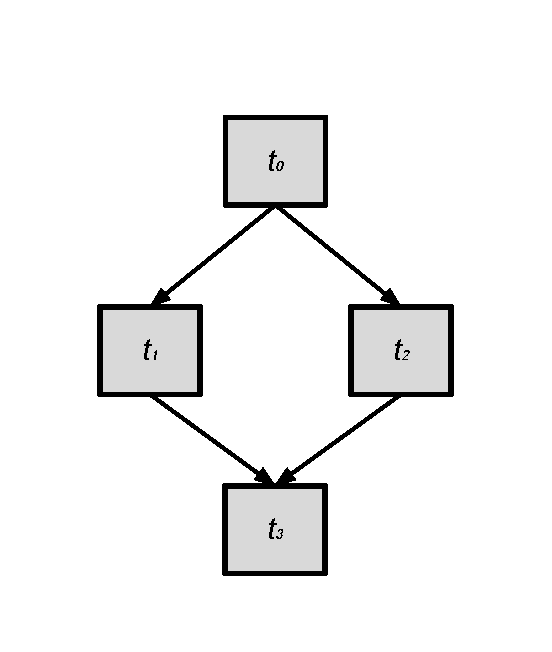
\includegraphics[width=0.5\textwidth]{figures/model/dag.pdf}
    \caption{A simple DAG with four tasks ($t_0$, $t_1$, $t_2$, $t_3$). The edges represent the data dependencies between tasks.}
    \label{fig:model_dag}
\end{figure}

\begin{figure}[h!]
	\centering
    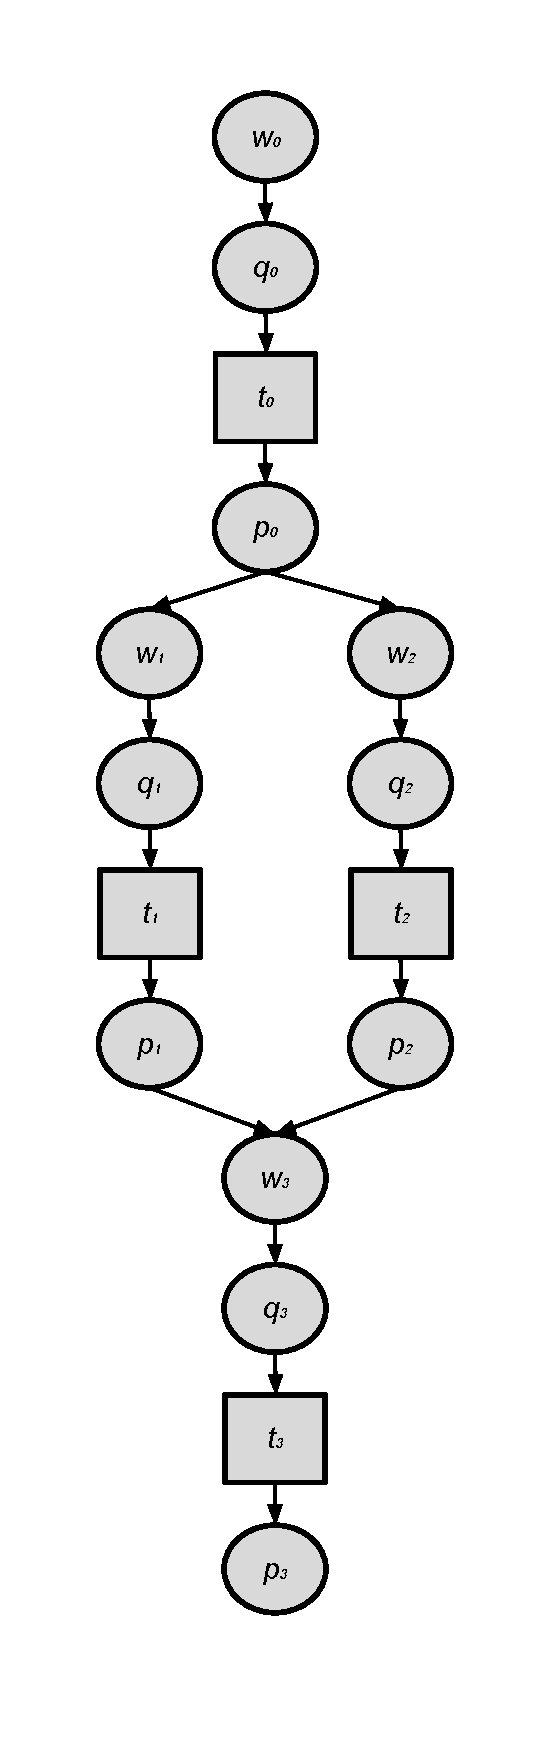
\includegraphics[width=0.4\textwidth]{figures/model/odag_before.pdf}
    \caption{An o-DAG with overheads ($w_0$$\sim$  $w_3$, $q_0$$\sim$  $q_3$, $p_0$$\sim$  $p_3$). The edges represent control dependencies or data dependencies}
    \label{fig:model_odag_before}
\end{figure}

Traditionally a workflow is modeled as a Directed Acyclic Graph (DAG). Each node in the DAG represents a workflow task, and the edges represent dependencies between the tasks ($t$) that constrain the order in which the tasks are executed. Each task is a program and a set of parameters that need to be executed. Fig~\ref{fig:model_dag} shows a simple workflow with four tasks. A job ($j$) is a single execution unit and it contains one or multiple task(s). The dependencies typically represent data flow dependencies in the application, where the output files produced by one task are needed as inputs of another task. 
%In this paper, we extend the DAG model to be overhead aware (o-DAG). The reason is that system overheads play an important role in workflow execution and they constitute a major part of the overall runtime when tasks are poorly clustered. 
Fig~\ref{fig:model_odag_before} shows how we augment a DAG in Fig~\ref{fig:model_dag} to be an o-DAG with the capability to represent scheduling overheads ($s$) such as workflow engine delay ($w$), queue delay ($q$), and postscript delay ($q$). Fig~\ref{fig:model_odag_after} further shows how we perform task clustering in this simple workflow, in which we merge $t_1$ and $t_2$ into a new job $j_4$. The scheduling overheads associated with $t_1$ and $t_2$ are removed and the overheads including the clustering delay ($c_4$) of $j_4$ are added. 

%To execute this workflow, a workflow engine such as DAGMan \cite{DAGMan} processes this DAG starting from the root task ($t_0$) and then executes each task without violating the data dependencies. Take the example of one available resource, a possible schedule would be $t_0\rightarrow t_1\rightarrow t_2\rightarrow t_3$ or $t_0\rightarrow t_2\rightarrow t_1\rightarrow t_3$. Both of the two schedules satisfy the data dependencies are thereby they are correct. 






The classification of overheads is based on the model of a typical workflow management system (WMS) shown in Fig~\ref{fig:model_system}. The components in this WMS are listed below: 




\begin{figure}[h!]
\centering
  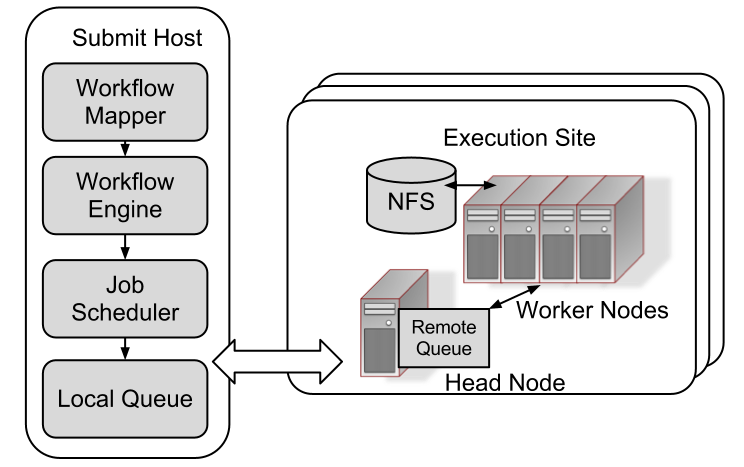
\includegraphics[width=0.6\linewidth]{figures/introduction/system.png}

  \caption{System Model}
  \label{fig:model_system}
\end{figure}


\textbf{Workflow Mapper} generates an executable workflow based on an abstract workflow provided by the user or a workflow composition system. 

\textbf{Workflow Engine} executes the jobs in order of their dependencies. Only free jobs that have all their parent jobs completed are submitted to  Job Scheduler. 

\textbf{Job Scheduler} and \textbf{Local Queue} manage individual workflow jobs and supervise their execution on local and remote resources.

\textbf{Job Wrapper} extracts tasks from clustered jobs and executes them at the worker nodes. 


\begin{figure}[h!]
	\centering
    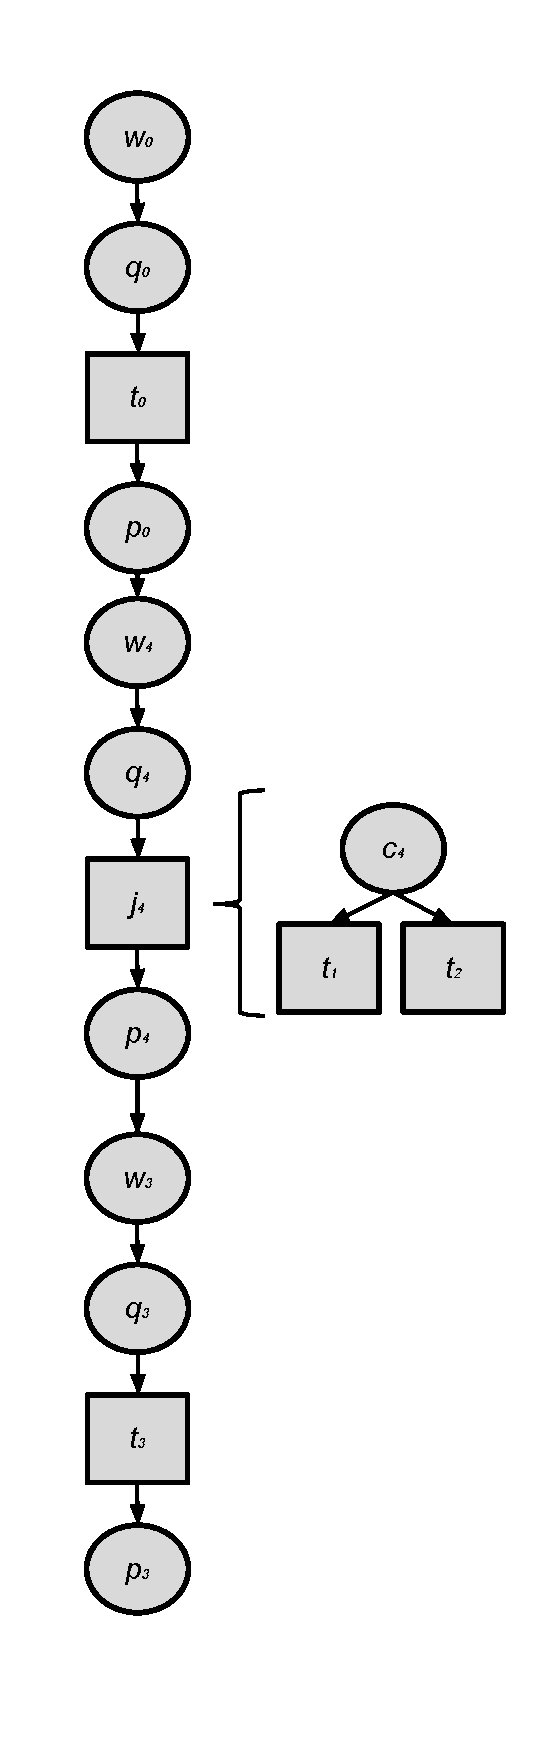
\includegraphics[width=0.4\textwidth]{figures/model/odag_after.pdf}
    \caption{ A Diamond Workflow after Task Clustering}
    \label{fig:model_odag_after}
\end{figure}


%An overhead is defined as the time of performing miscellaneous work other than executing the user’s computational activities. 
%The execution of scientific workflows often suffers from a variety of overheads in the distributed environment. 
%Due to the distributed nature of these resources, the large number of tasks in a workflow, and the complex dependencies among the tasks, significant overheads can occur during the workflow execution. 
%It is essential to identify the different overheads and to evaluate how different optimization methods reduce overheads and improve runtime performance. 
%In this section, we present an overhead analysis for a set of workflows run on cloud, grid, or cluster platforms. 
%We present the overhead distributions and the patterns that they have performed. 

\subsection{Overhead Classification}


\begin{figure}[h!]
	\centering
    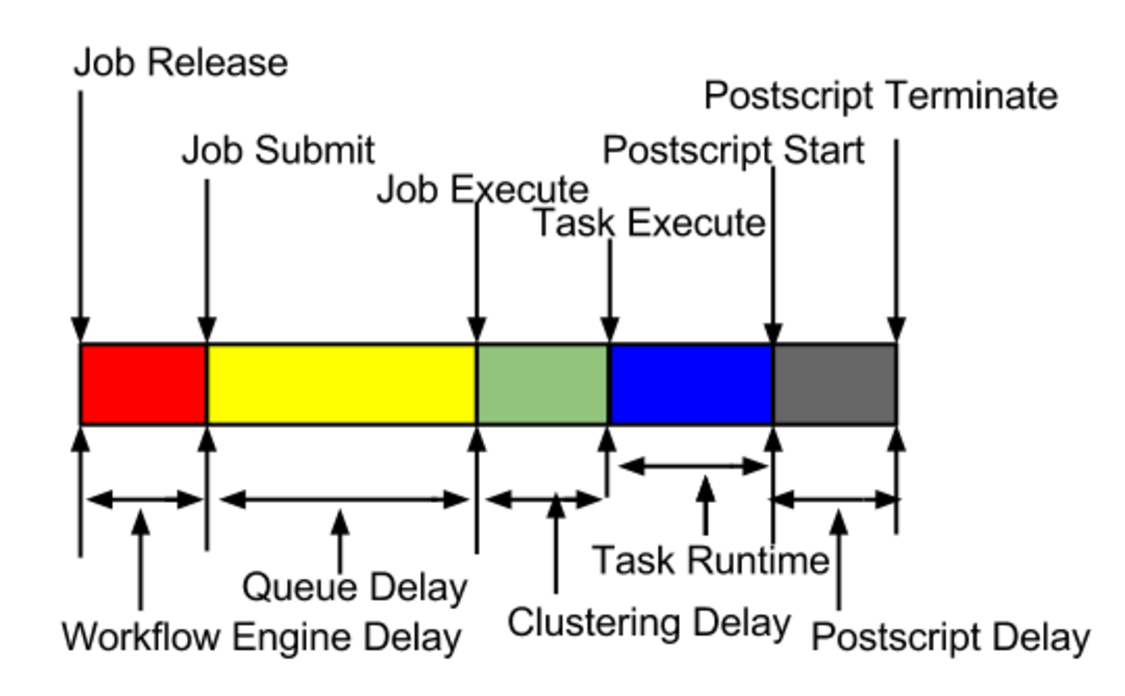
\includegraphics[width=0.7\textwidth]{figures/model/overhead.pdf}
    \caption{Workflow Events}
    \label{fig:model_overhead}
\end{figure}


The execution of a job is comprised of a series of events as shown in Figure~\ref{fig:model_overhead} and they are defined as:
\begin{enumerate}
\item Job Release is defined as the time when the workflow engine identifies that a job is ready to be submitted (when its parents have successfully completed). 
\item Job Submit is defined as the time when the workflow engine submits a job to the local queue. 
\item Job Execute is defined as the time when the workflow engine sees a job is being executed. 
\item Task Execute is defined as the time when the job wrapper sees a task is being executed. 

\item Postscript Start is defined as the time when the workflow engine starts to execute a postscript. 
\item Postscript Terminate is defined as the time when the postscript returns a status code (success or failure). 
\end{enumerate}

Figure~\ref{fig:model_overhead} shows a typical timeline of overheads and runtime in a compute job. We do not specify the data transfer delay in this timeline because data transfer is handled by data transfer jobs (stage-in and stage-out jobs). 

We have classified workflow overheads into five categories as follows. 
\begin{enumerate}

\item{Workflow Engine Delay} measures the time between when the last parent job of a job completes and the time when the job gets submitted to the local queue. 
%In case of retries the value of the last retry is used for the calculation. 
The completion time of the last parent job means this job is released to the ready queue and is waiting for resources to be assigned to it. The workflow engine delay reflects the efficiency of a workflow engine (i.e., DAGMan \cite{DAGMan}). 

\item{Queue Delay} is defined as the time between the submission of a job by the workflow engine to the local queue and the time the local scheduler sees the job running. This overhead reflects the efficiency of the local workflow scheduler (e.g. Condor \cite{Frey2002}) to execute a job and the availability of resources for the execution of this job. 
%The queue delay is an estimate of the time spent in the local queue on the submit host. 

\item{Postscript Delay } is the time taken to execute a lightweight script under some execution systems after the execution of a job. Postscripts examine the status code of a job after the computational part of this job is done.

%\item{Data Transfer Delay} happens when data is transferred between nodes. It includes three different types of processes: staging data in, cleaning up, and staging data out. Stage-in jobs transfer input files from source sites to execution sites before the computation starts. Cleanup jobs delete intermediate data that is no longer needed by the remainder of the workflow. Stage-out jobs transfer workflow output data to archiving sites for storage and analysis.

\item{Clustering Delay} measures the difference between the sum of the actual task runtime and the job runtime seen by the job wrapper. The cause of Clustering Delay is usually because we use a job wrapper in worker nodes to execute a clustered job that requires some delay to extract the list of tasks. 
\end{enumerate}

\subsection{Overhead Distribution}

%We examined the overhead distributions of a wide range of workflows in our experiments . These workflows were run on distributed platforms including clouds, grids and dedicated clusters. 
%%On clouds, virtual machines were provisioned and then the required services (such as file transfer services) were deployed. 
%We examined two clouds: Amazon EC2 \cite{AmazonEC2}  and FutureGrid \cite{FutureGrid}. Amazon EC2 is a commercial, public cloud that is been widely used in distributed computing. 
We examined the overhead distributions of a widely used astronomy workflow called Montage \cite{Berriman2004} that is used to construct large image mosaics of the sky. Montage was run on FutureGrid \cite{FutureGrid}. FutureGrid is a distributed, high-performance testbed that provides scientists with a set of computing resources to develop parallel, grid, and cloud applications. 
%%On grids, grid resources were provisioned through Corral \cite{Juve2010a} and the required services were already installed before execution. A grid site may be a cluster system or a heterogeneous and dynamic collection of machines. In a dedicated cluster, Condor was used to schedule jobs directly to worker nodes. Part of this experimental data (especially those workflows run on Amazon EC2) has been studied in \cite{Juve2010c} but without a detailed overhead analysis. 
%For the Amazon EC2 experiments, the performance with different numbers of resources and file system types is compared.
%The workflows and execution environments we examined include:
%\begin{enumerate}
%%\item Epigenomics \cite{Epigenome} maps short DNA segments collected with high-throughput gene sequencing machines to a reference genome. It was run on Amazon EC2. 

%%\item Proteomics \cite{Proteomics} is an application developed by scientists at Ohio State University and it is used for mass-spectrometry-based proteomics. It was run on Amazon EC2. 

%\item Broadband \cite{Graves2008} is an application that enables researchers to combine long-period deterministic seismograms with high-frequency stochastic seismograms. It was run on Amazon EC2. 

%\item Montage \cite{Berriman2004} is an astronomy application used to construct large image mosaics of the sky. The Montage workflows were run on FutureGrid.

%\item CyberShake \cite{Graves2010, Callaghan2008, Deelman2006} is a seismology application that calculates Probabilistic Seismic Hazard curves for geographic sites in the Southern California region. It was run on the HPCC cluster \cite{HPCC} at the University of Southern California. 

%\item SIPHT \cite{Livny2008} conducts searches for small untranslated RNAs (sRNAs) that are used to regulate essential biochemical processes in bacteria. It was run on a Condor cluster at the University of Wisconsin at Madison. 

%\item LIGO \cite{Abramovici1992,LIGO} workflows are used to search for gravitational wave signatures in data collected by large-scale interferometers. We present one partition of the entire workflow in this work. It was run on a local cluster at the Syracuse University.
%\end{enumerate}
%
%\begin{figure}[h!]
%	\centering
%    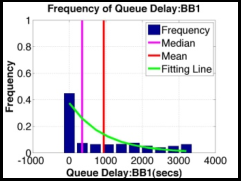
\includegraphics[width=0.4\textwidth]{figures/model/BB1.pdf}
%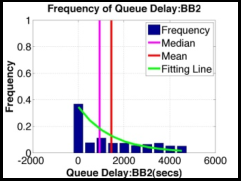
\includegraphics[width=0.4\textwidth]{figures/model/BB2.pdf}
%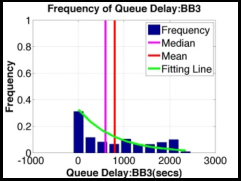
\includegraphics[width=0.4\textwidth]{figures/model/BB3.pdf}
%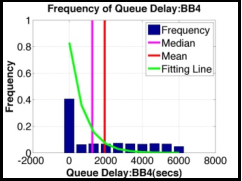
\includegraphics[width=0.4\textwidth]{figures/model/BB4.pdf}
%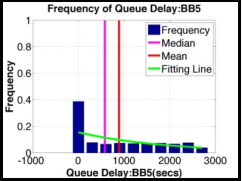
\includegraphics[width=0.4\textwidth]{figures/model/BB5.pdf}
%    \caption{Frequency Distribution of Queue Delay in Broadband}
%    \label{fig:model_broadband_distribution}
%\end{figure}
%
%\begin{table}[h!]
%\caption{Makespan of Broadband}
%\label{tab:model_broadband}
%\centering
%\begin{tabular}{lrrrr}
%\hline
%     &      Makespan &     Num of Nodes &    File System  \\
%\hline
%BB1 & 1:08:17 & 8 & NFS\\
%BB2 & 1:29:23 & 4 & NFS \\
%BB3 & 1:32:57 & 4 & PVFS \\
%BB4 & 1:51:14 & 1 & NFS \\
%BB5 & 0:52:48 & 1 & shm \\
%\hline
%\end{tabular}
%\end{table} 
%
%\begin{table}[h!]
%\caption{the SSE (sum of squares of error) of different fitting distribution}
%\label{tab:model_broadband_sse}
%\centering
%\begin{tabular}{lrrrr}
%\hline
%SSE(Unit: $10^4$)     &      Exponential &  Gamma & Normal & Weibull \\
%\hline
%BB1 & 3.57 & 232 & 8.69 & 235.2\\
%BB2 & 2.33 & 244 & 5.59 & 181.0\\
%BB3 & 1.97 & 73.9 & 4.18 & 52.4\\
%BB4 & 3.31 & 340 & 7.22 & 251.7\\
%BB5 & 2.84 & 73.1 & 6.48 & 55.4 \\
%\hline
%\end{tabular}
%\end{table} 
%
%\begin{table}[h!]
%\caption{the $\mu$ of the exponential fitting distribution}
%\label{tab:model_broadband_mu}
%\centering
%\begin{tabular}{lrrrr}
%\hline
%(Unit: sec)     &      $\mu$ \\
%\hline
%BB1 & 944.85\\
%BB2 & 1451.88\\
%BB3 & 796.90\\
%BB4 & 1952.71\\
%BB5 & 892.16 \\
%\hline
%\end{tabular}
%\end{table} 
%
%\begin{table}[h!]
%\caption{the log likelihood of different fitting distribution}
%\label{tab:model_broadband_log}
%\centering
%\begin{tabular}{lrrrr}
%\hline
%Log Likelihood     &      Exponential &  Gamma & Normal & Weibull \\
%\hline
%BB1 & -6045.3 & -5802.3 & -6464.1 & -5819.6\\
%BB2 & -6376.1 & -6203.1 & -6707.9 & -6232.9\\
%BB3 & -5914.2 & -5796.4 & -6181.4 & -5825.9\\
%BB4 & -6376.1 & -6203.1 & -6707.9 & -6232.9\\
%BB5 & -6001.1 & -5891.9 & -6327.9 & -5908.1 \\
%\hline
%\end{tabular}
%\end{table} 
%
%Frequency distribution analysis serves as an important supplement to the understanding of how different execution environments influence the overheads. Figure~\ref{fig:model_broadband_distribution} presents the mean, median and the exponential fitting lines of Queue Delay in Broadband of five runs (BB1$\sim$BB5). The Broadband workflows were executed in environments with different number of worker nodes and file systems. These runs had the same jobs and used the same type of virtual machines (c1.xlarge), but they were run in different environments. The number of worker nodes was ranging from 1 to 8 and the file systems included NFS \cite{Sandberg1985}, PVFS \cite{Carns2000} and a shared memory system (shm) on a single host. 
%
%Comparing BB1, BB2 and BB4 we conclude that resource availability influences the distribution of the queue delay. Although for all the five runs, most of the queue delays (30\%$\sim$40\%) last less than 50 seconds, the maximum duration of queue delay increases with the decrease of resource availability. With more resources available, the local scheduler is able to find a resource for execution more quickly. BB3 is installed with PVFS, which performs worse than BB2 with NFS in this experiment. The shared memory system can also improve the performance, but it is limited to the case with only one host.  
%
%We use the Matlab Distribution Fitting tool \cite{Matlab} to analyze the distribution of the queue delay. This tool aims to maximize the log likelihood of the parameters. Table~\ref{tab:model_broadband_log} shows that the queue delay satisfies the Weibull and Gamma distribution better in terms of the log likelihood. However, Table~\ref{tab:model_broadband_sse} shows that in terms of SSE (sum of squares of error), the exponential and normal distributions perform better. For simplicity, we use an exponential distribution to describe the queue delay:
%
%\begin{equation} \label{eq:model_f1}
% \phi_1(x)=\frac{1}{\mu}e^{-\frac{x}{\mu}}\varepsilon(x)
%\end{equation}
%
%$\varepsilon(x)$ is an unit step function. The estimates of $\mu$ are listed in Table~\ref{tab:model_broadband_mu}. 

%Figure~\ref{fig:model_cybershake_distribution} shows the mean and standard deviation of all 78 partitions of the entire CyberShake workflow. The standard deviation is comparable to the mean of the overheads, which we attribute to the fact that HPCC comprises a diverse mix of computing and data resources and is shared among many users across the campus. 
Figure~\ref{fig:model_montage_distribution} shows the overhead distribution of the Montage workflow run on the FutureGrid. The postscript delay concentrates at 7 seconds, because the postscript is only used to locally check the return status of a job and is not influenced by the remote execution environment. The workflow engine delay tends to have a uniform distribution, which is because the workflow engine spends a constant amount of time to identify that the parent jobs have completed and insert a job that is ready at the end of the local queue. 
%Normally, the queue delay has only one peak such as in Figure~\ref{fig:model_broadband_distribution}. But in this experiment, 
The queue delay has three decreasing peak points at 8, 14, and 22 seconds. We believe this is because the average postscript delay is about 7 seconds (see details in Figure~\ref{fig:model_montage_distribution} ) and the average runtime is 1 second. The local scheduler spends about 8 seconds finding an available resource and executing a job; if there is no resource idle, it will wait another 8 seconds for the current running jobs to finish, and so on. 
%Based on Equation~\ref{eq:model_f1}, an integrated function of the queue delay can be expressed as a combination of multiple exponential distributions:
%\begin{equation} \label{eq:model_f2}
% \phi_2(x)=\sum_{i=1}^{\infty}e^{-ai}\phi_1(x-ib)
%\end{equation}
%$a$ is the attenuation coefficient of the exponential distribution and $b$ is the average distance between the peaks, namely the period. In the example of Figure~\ref{fig:model_montage_distribution}, $a\approx0.5, b\approx7$. 

%\begin{figure}[h!]
%	\centering
%    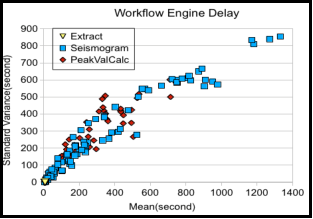
\includegraphics[height=0.3\textwidth]{figures/model/cybershake_engine_delay.pdf}
%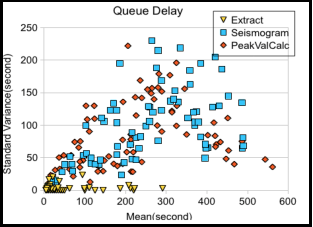
\includegraphics[height=0.3\textwidth]{figures/model/cybershake_queue_delay.pdf}
%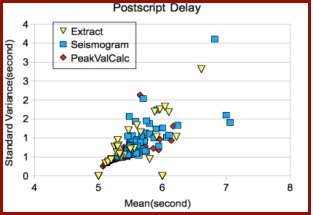
\includegraphics[width=0.4\textwidth]{figures/model/cybershake_post_delay.pdf}
%
%    \caption{Mean and Variance of all the 78 partitions of the CyberShake workflow}
%    \label{fig:model_cybershake_distribution}
%\end{figure}

\begin{figure}[h!]
	\centering
    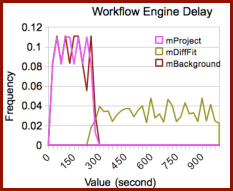
\includegraphics[height=0.3\textwidth]{figures/model/montage_engine_delay.pdf}
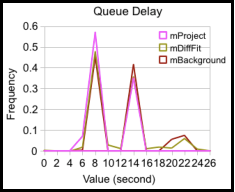
\includegraphics[height=0.3\textwidth]{figures/model/montage_queue_delay.pdf}
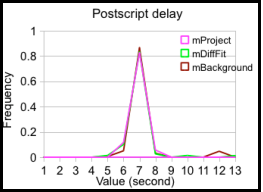
\includegraphics[width=0.4\textwidth]{figures/model/montage_post_delay.pdf}

    \caption{Distribution of overheads in the Montage workflow}
    \label{fig:model_montage_distribution}
\end{figure}

%In our prior work \cite{Overhead2011}, we have introduced the distribution of overheads and the relationship between them. Following this, we indicate the necessity to consider the distribution of overheads rather than simply adding a constant delay after job execution. 
We use Workflow Engine Delay as an example to show the necessity to model overheads appropriately. Figure~\ref{fig:model_montage_timeline} shows a real trace of overheads and runtime in the Montage 8 degree workflow (for visibility issues, we only show the first 15 jobs at the mProjectPP level). We can see that Workflow Engine Delay increases steadily after every five jobs. For example, the Workflow Engine Delay of jobs with ID from 6 to 10 is approximately twice of that of jobs ranging from ID1 to ID5. Figure~\ref{fig:model_montage_five_runs} further shows the distribution of Workflow Engine Delay at the mProjectPP level in the Montage workflow that was run five times. After every five jobs, the Workflow Engine Delay increases by 8 seconds approximately. We call this special nature of workflow overhead as cyclic increase. The reason is that Workflow Engine (in this trace it is DAGMan) releases five jobs by default in every working cycle. Therefore, simply adding a constant delay after every job execution has ignored its potential influence on the performance.

\begin{figure}[h!]
	\centering
    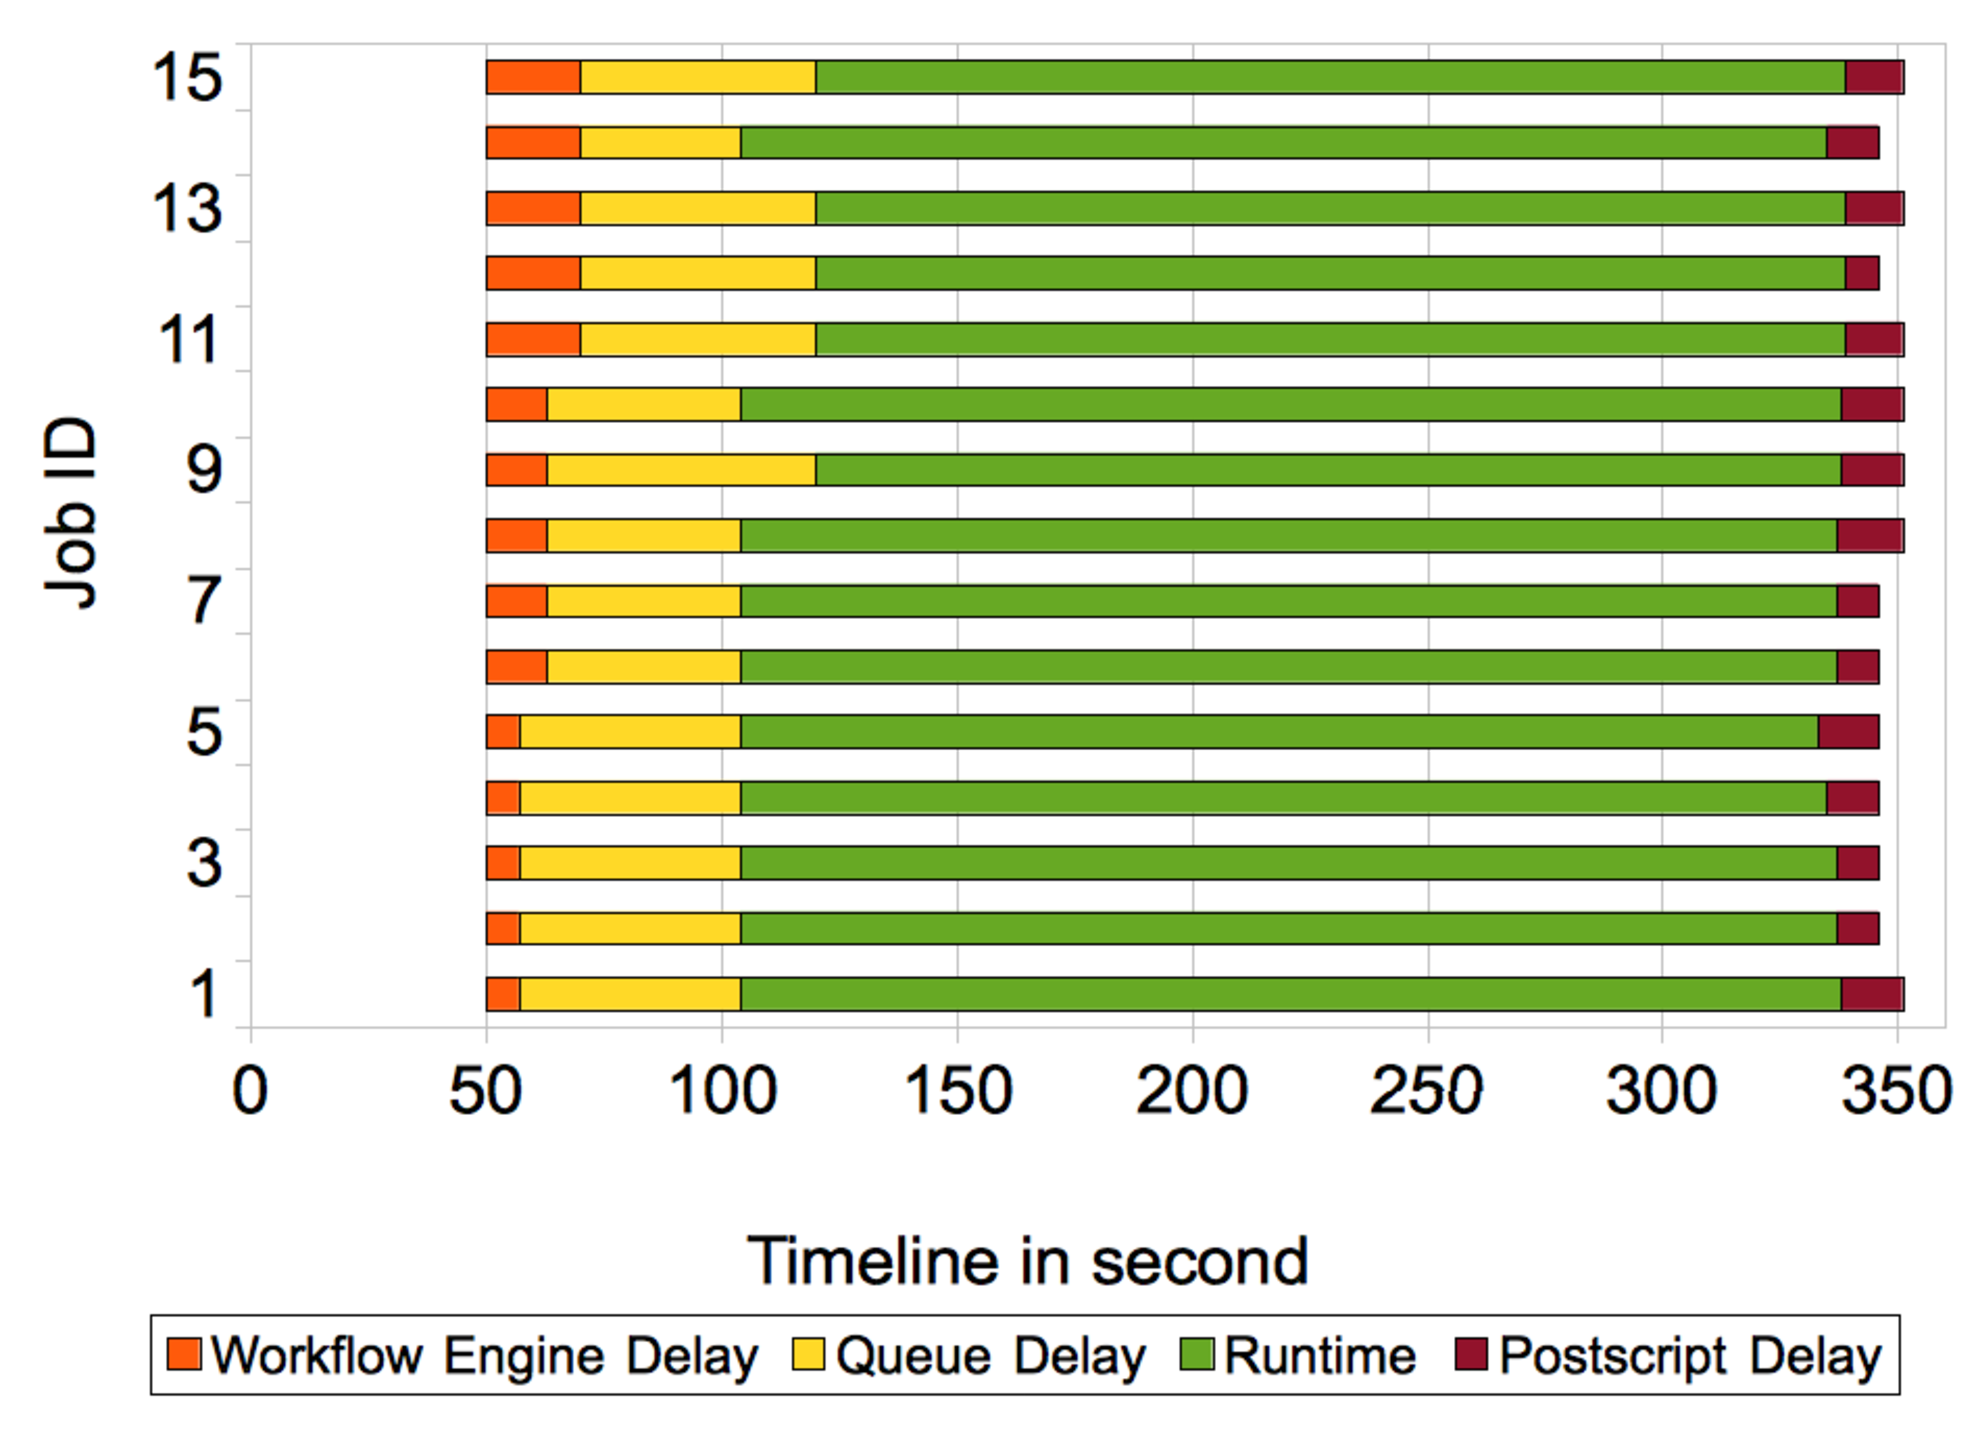
\includegraphics[width=0.7\textwidth]{figures/model/overhead_timeline2.pdf}
    \caption{Workflow Overhead and Runtime. Clustering delay and data transfer delay are not shown}
    \label{fig:model_montage_timeline}
\end{figure}




\begin{figure}

\centering
  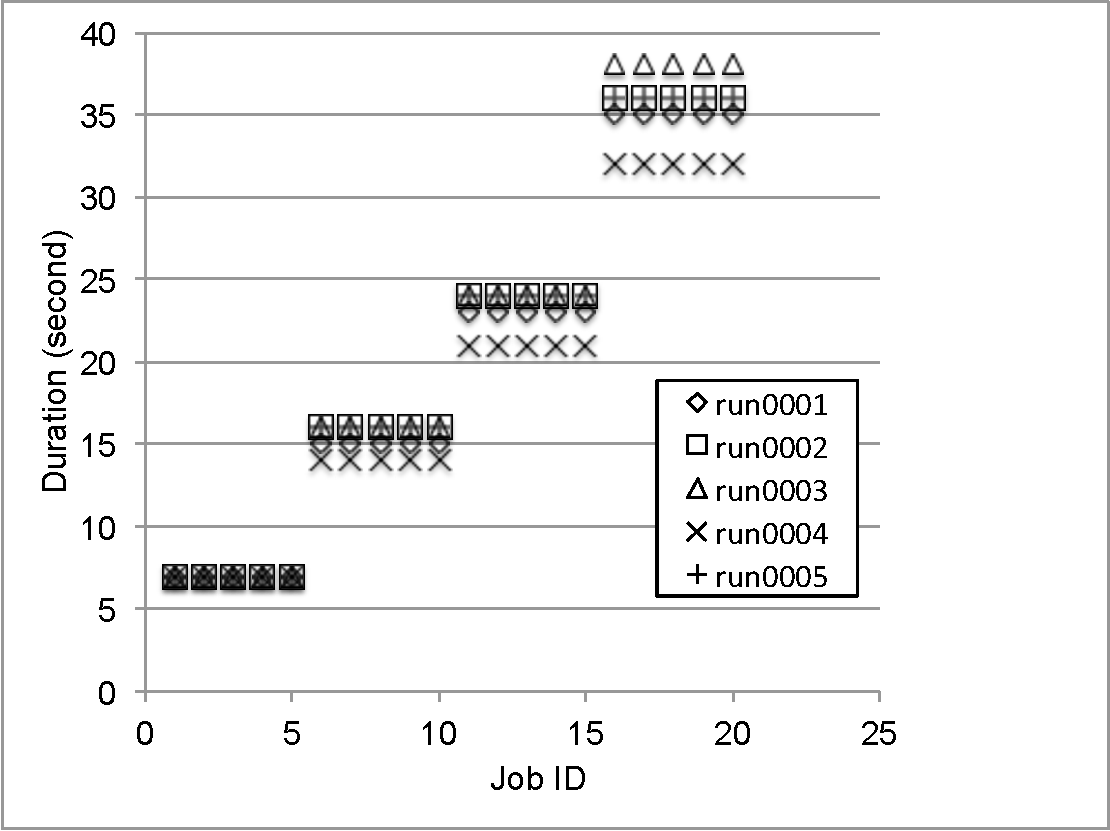
\includegraphics[width=0.6\linewidth]{figures/model/montage_five_runs.pdf}
    \caption{Workflow Engine Delay of mProjectPP}
    \label{fig:model_montage_five_runs}
\end{figure}%
\begin{figure}
  \centering
  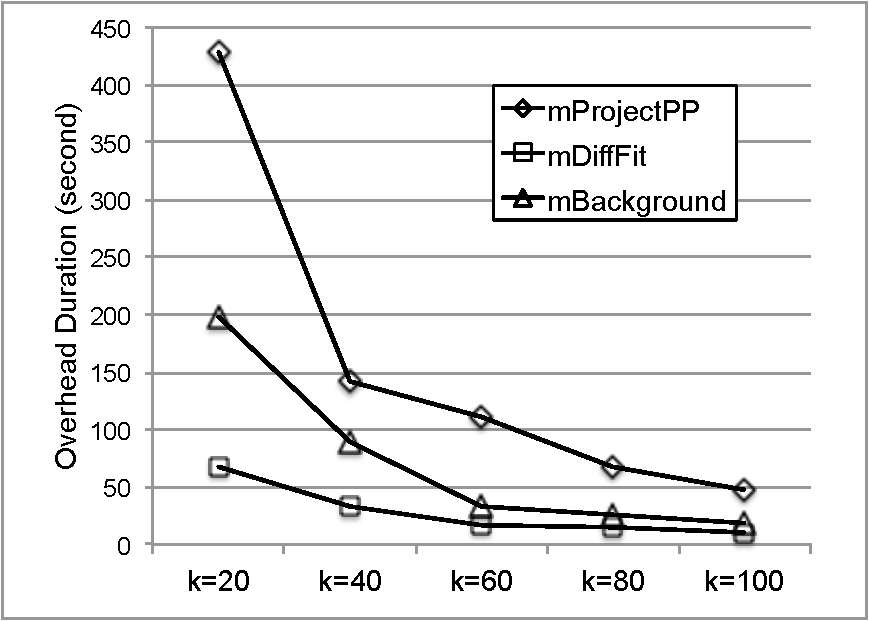
\includegraphics[width=0.6\linewidth]{figures/model/montage_clustering_delay.pdf}
    \caption{Clustering Delay of mProjectPP, mDiffFit, and mBackground}
    \label{fig:model_montage_clustering}
\end{figure}





Figure~\ref{fig:model_montage_clustering} shows the average value of Clustering Delay of mProjectPP, mDiffFit, and mBackground. It is clear that with the increase of $k$ (the maximum number of jobs per horizontal level), since there are less and less tasks in a clustered job, the Clustering Delay for each job decreases. For simplicity, we use an inverse proportional model in Equation~\ref{eq:model_clustering_delay} to describe this trend of Clustering Delay with $k$. Intuitively we assume that the average delay per task in a clustered job is constant ($n$ is the number of tasks in a horizontal level). An inverse proportional model can estimate the delay when $k=i$ directly if we have known the delay when $k=j$. Therefore we can predict all the clustering cases as long as we have gathered one clustering case. 

\begin{equation} \label{eq:model_clustering_delay}
\frac{Clustering Delay|_{k=i}}{Clustering Delay|_{k=j}}=\frac{n/i}{n/j}=\frac{j}{i}
\end{equation}



\subsection{Metrics to Evaluate Cumulative Overheads}

After identifying the major overheads in workflows and describe how they are measured based on workflow events, we provide an integrated and comprehensive quantitative analysis of workflow overheads. The observation on overhead distribution and characteristics enable researchers to build a more realistic model for simulations of real applications. Our analysis also offers guidelines for developing further optimization methods. 

%We propose several metrics to calculate the cumulative sum of the overheads based on how they overlap and their importance in the graph. In addition, we indicate how experimental parameters impact the overhead and thereby the overall workflow performance. We then show how popular optimization methods improve runtime performance by reducing some or all types of overheads. 

In this section, we define four metrics to calculate cumulative overheads of workflows, which are $Sum$, $Projection(PJ)$, $Exclusive~Projection(EP)$ and $Reverse~Ranking(RR)$. $Sum$ simply adds up the overheads of all jobs without considering their overlap. $PJ$ subtracts from $Sum$ all overlaps of the same type of overhead. It is equal to the projection of all overheads to the timeline. $EP$ subtracts the overlap of all types of overheads from $PJ$. It is equal to the projection of overheads of a particular type excluding all other types of overheads to the timeline.
$RR$ uses a reverse ranking algorithm to index overheads and then calculates the cumulative overhead weighted by the ranks. The idea is brought by web page indexing algorithms such as PageRank \cite{PageRank1999}. Figure~\ref{fig:model_rr} shows how to calculate the reverse ranking value $(RR)$ of the same workflow graph in Figure~\ref{fig:model_overhead_timeline}.
 
\begin{equation} \label{eq:model_rr}
RR(j_u)=d+(1-d)\times\sum_{j_v\in Child(j_u)}{}\frac{RR(j_v)}{L(j_v)}
\end{equation}

Equation~\ref{eq:model_rr} means that the $RR$ of a node (overhead or job) is determined by the $RR$ of its child nodes. $d$ is the damping factor, which usually is 0.15 as in PageRank. $L(j_v)$ is the number of parents that node $j_v$ has. Intuitively speaking, a node is more important if it has more child nodes and its child nodes are more important. In terms of workflows, it means an overhead has more power to control the release of other overheads and computational activities. There are two differences compared to the original PageRank: 
\begin{enumerate}
\item We use output link pointing to child nodes while PageRank uses input link from parent nodes, which is why we call it reverse ranking algorithm.
\item Since a workflow is a DAG, we do not need to calculate $RR$ iteratively. For simplicity, we assign the $RR$ of the root node to be 1. And then we calculate the $RR$ of a workflow ($G$) based on the equation below:

\begin{equation} \label{eq:model_sum_rr}
RR(G)=\sum_{}{}RR(j_u) \times \phi_{j_u}
\end{equation}

\end{enumerate}
 
$\phi_{j_u}$ indicates the duration of job $j_u$.  $RR$ evaluates the importance of an overhead and represents the cumulative overhead weighted by this importance. 
The reason we have four metrics of calculating cumulative overheads is to present a comprehensive overview of the impact of overlaps between the various overheads and runtime. Many optimization methods such as Data Placement Services \cite{Amer2012} try to overlap overheads and runtime to improve the overall performance. By analyzing these four types of cumulative overheads, researchers have a clearer view of whether their optimization methods have overlapped the overheads of a same type (if $PJ < Sum$) or other types (if $EP < PJ$). $RR$ shows the connectivity within the workflow, the larger the denser. 
We use a simple example workflow with three jobs to show how to calculate the overlap and cumulative overheads. Figure~\ref{fig:model_overhead_timeline} shows the timeline of our example workflow. Job1 is a parent job of Job 2 and Job 3.

\begin{figure}[h!]
	\centering
    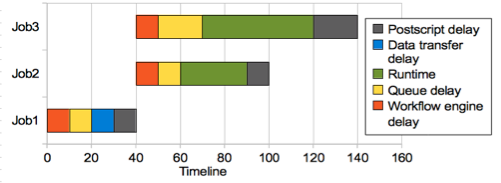
\includegraphics[width=0.6\textwidth]{figures/model/overhead_timeline.pdf}
    \caption{The Timeline of an Example Workflow}
    \label{fig:model_overhead_timeline}
\end{figure}
\begin{figure}[h!]
	\centering
    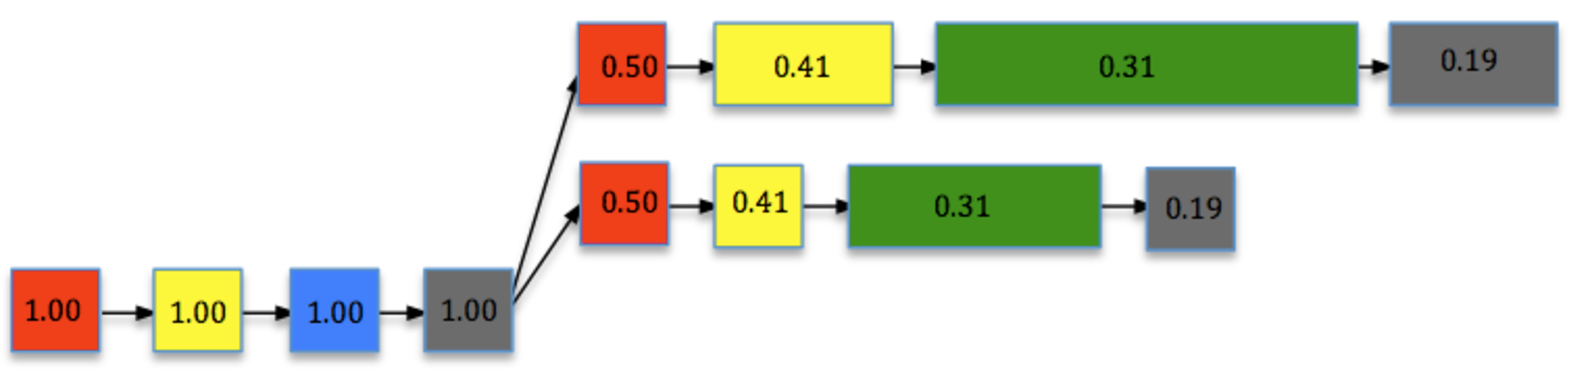
\includegraphics[width=0.7\textwidth]{figures/model/rr.pdf}
    \caption{Reverse Ranking}
    \label{fig:model_rr}
\end{figure}
At $t=0$, job 1, a stage-in job, is released: $queue~delay = 10$, $workflow~engine~delay = 10$, $runtime = 10$, and $postscript~delay = 10$.
At $t=40$, job 3 is released: $workflow~engine~delay = 10$, $queue~delay = 20$, $runtime = 50$, and $postscript~delay = 20$.
At $t=40$, job 2 is released: $workflow~engine~delay = 10$, $queue~delay = 10$, $runtime = 30$, $postscript~delay = 10$. 

%We show how to calculate the cumulative overheads:
 
%For $Sum$:
%$Sum(runtime)=50+30=80$. It contains the time slots of [60, 90] and [70, 120]. 
%$Sum(queue~delay)=10+20+10=40$. It contains [10, 20], [50, 70] and [50, 60]. 
%$Sum(workflow~engine~delay)=10+10+10=30$. It contains [0,10], [40, 50] and [40, 50]. 
%$Sum(postscript~delay)=10+20+10=40$. It contains [30, 40], [90, 100] and [120, 140]. 
%$Sum(data~transfer~delay)=10$. It contains [20, 30].

%For $PJ$:
%$PJ(runtime)=50+30-20=60$. It contains [60, 120].
%$PJ(queue~delay)=10+20+10-10=30$. It contains [10, 20] and [50, 70].
%$PJ(workflow~engine~delay)=10+10+10-10=20$. It contains [0, 10] and [40, 50].
%$PJ(postscript~delay)=10+20+10=40$. It contains [30, 40], [90, 100] and [120, 140].
%$PJ(data~transfer~delay)=10$. It contains [20, 30].

%For $EP$: 
%$EP(runtime)=50+30-20-10-10=40$. It contains [70, 90] and [100, 120].
%$EP(queue~delay)=10+20+10-10-10=20$. It contains [10, 20] and [50, 60]. 
%$EP(workflow~engine~delay)=10+10+10-10=20$. It contains [0, 10] and [40, 50]. 
%$EP(postscript~delay)=10+20+10-10=30$. It contains [30, 40] and  [120,140]. 
%$EP(data~transfer~delay)=10$. It contains [20, 30].

%$RR(runtime)=50\times 0.31+30\times 0.31=24.8$.
%$RR(queue~delay)=10\times 1.00+10\times 0.41+10\times 0.41=18.2$.
%$RR(workflow~engine~delay)=10\times 1.00+10\times 0.50+10\times 0.50=20$.
%$RR(postscript~delay)=10\times 1.00+10\times 0.19+20\times 0.19=15.7$.
%$RR(data~transfer~delay)=10\times 1.00=10$.

In calculating the cumulative runtime, we do not include the runtime of stage-in jobs because we have already classified it as data transfer delay. The overall makespan for this example workflow is 140. Table~\ref{tab:model_percentage_overhead} shows the percentage of overheads and job runtime over makespan.  

\begin{table}[h!]
\caption{Percentage of Overheads and Runtime}
\label{tab:model_percentage_overhead}
\centering
\begin{tabular}{lrrrr}
\hline
Percentage & Sum & PJ & EP &RR\\

\hline

runtime & 57.14\% & 42.86\% & 28.57\% &17.71\% \\
queue delay & 28.57\% &21.43\% &14.29\% &13.00\% \\
workflow engine delay & 21.43\% &14.29\%& 14.29\% &14.29\%\\
postscript delay & 28.57\% & 28.57\% & 21.43\% & 11.21\% \\
data transfer delay & 7.14\% & 7.14\% & 7.14\% & 7.14\% \\
sum & 142.86\% & 114.29\% & 85.71\% & 63.36\%\\
\hline
\end{tabular}
\end{table} 


In Table~\ref{tab:model_percentage_overhead}, we can conclude that the sum of $Sum$ is larger than makespan and smaller than makespan$\times$(number of resources) because it does not count the overlap at all. $PJ$ is larger than makespan since the overlap between more than two types of overheads may be counted twice or more. $EP$ is smaller than makespan since some overlap between more than two types of overheads may not be counted.  $RR$ shows how intensively these overheads and computational activities are connected to each other. 

%Should be included in final defense
%\subsection{Relationship between Overhead Metrics and Overall Performance}

%In this section, we aim to investigate the relationship between the overhead metrics that we proposed and the overall performance of popular workflow restructuring techniques. Among them, task clustering \cite{Singh2008} is a technique that increases the computational granularity of tasks by merging small tasks together into a clustered job, reducing the impact of the queue wait time and also the makespan of the workflow. Data or job throttling \cite{Humphrey2008} limits the amount of parallel data transfer to avoid overloading supporting services such as data servers. Throttling is especially useful for unbalanced workflows in which one task might be idle while waiting for data to arrive. The aim of throttling is to appropriately regulate the rate of data transfers between the workflow tasks via data transfer servers by ways of restricting the data connections, data threads or data transfer jobs. Provisioning tools often deploy pilot jobs as placeholders for the execution of application jobs. Since a placeholder can allow multiple application jobs to execute during its lifetime, some job scheduling overheads can be reduced. 

%\textbf{How Task Clustering Reduces Overheads}

%In the following sections, we use a Montage workflow to show how different optimization methods improve overall performance. Many workflows are composed of thousands of fine computational granularity tasks. Task clustering is a technique that increases the computational granularity of tasks by merging small jobs together into a clustered job, reducing the impact of the queue wait time and minimizing the makespan of the workflow. Table 4.2 compares the overheads and runtime of the Montage workflow. We can conclude that with clustering, although the average overheads do not change much, the cumulative overheads decrease greatly due to the decreased number of jobs. With clustering, the makespan has been reduced by 53.3\% by reducing the number of all jobs from 3461 to 104 in this example. Figure 4.5 shows the percentage of workflow overheads and runtime. The percentage is calculated by the cumulative overhead ($PJ$, or $EP$) divided by the makespan of workflows. With clustering, the portion of runtime is increased significantly. Figure 4.6 profiles the number of active jobs during execution and it also shows that with clustering the resource utilization is improved significantly. 

%\textbf{How Job Throttling Reduces Overheads}

%Data or job throttling [13] limits the amount of parallel data transfer to avoid overloading supporting services such as data servers. Throttling is especially useful for unbalanced workflows in which one task might be idle while waiting for data to arrive. The aim of throttling is to appropriately regulate the rate of data transfers between the workflow tasks via data transfer servers by ways of restricting the data connections, data threads or data transfer jobs. Especially on cloud platforms, I/O requests need to go through more layers than a physical cluster; and thereby workflows may suffer a higher overhead from data servers.

%In our experiments, the data transfer service is deployed on a virtual machine that is similar to a worker node.  In this section, we evaluate a simple static throttling strategy where the Condor scheduler limits the number of concurrent jobs to be run and thereby restricts the number of parallel I/O requests. There are 32 resources available and we evaluate the cases with throttling parameters that are equal to 24, 16 and 12 in Table 4.3. In the case of 24, the resources are better utilized but the data server is heavily loaded. In the case of 12, the resources are under-utilized even though the data server has more capabilities. In this experiment, both $PJ$ and $EP$ reflect the variation trend of overheads and makespan better than $Sum$. 

%Figure 4.7 shows the percentage of workflow overheads and runtime. Figure 4.8 profiles the number of active jobs during execution. Montage is an unbalanced workflow because the three major types of jobs (mProjectPP, mDiffFit, and mBackground) impose a heavy load on the data server while the other jobs in the workflow do not. Figure 4.8 shows that with throttling the maximum number of active jobs is restricted. With limited throttling (reducing threshold from 24 to 16), the data transfer requests are distributed in the timeline more evenly and, as a result, their overhead is reduced. However, with over throttling (reducing threshold from 16 to 12), resources are not fully utilized and thus the makespan is increased. 

%\textbf{How Pre-staging Reduces Overheads}

%Scientific workflows often consume and produce a large amount of data during execution. Data pre-staging [14] transfers input data before the computational activities are started or even before the workflow is mapped onto resources. Data placement policies distribute data in advance by placing data sets where they may be requested or by replicating data sets to improve runtime performance. In our experiments, because data is already pre-staged, the implementation of the stage-in job is to create a soft link to the data from the workflow’s working directory, making it available to the workflow jobs. Table 4.4 and Figure 4.9 show the cumulative overheads and runtime of the Montage workflows running with and without pre-staging. Looking at the rows for $PJ$ in Table 4.4, we can conclude that pre-staging improves the overall runtime by reducing the data transfer delay. For the case without pre-staging the $EP$ for data transfer delay is zero because it overlaps with the workflow engine delay of another job. Therefore, in this experiment, $PJ$ reflects the variation trend of the makespan more consistently. 

%\textbf{How Provisioning Reduces Overheads}

%Many of the scientific applications presented here consist of a large number of short-duration tasks whose runtimes are greatly influenced by overheads present in distributed environments. Most of these environments have an execution mode based on batch scheduling where jobs are held in a queue until resources become available to execute them. Such a best-effort model normally imposes heavy overheads in scheduling and queuing. For example, Condor-G [23] uses Globus GRAM [37] to submit jobs to remote clusters. The Globus Toolkit normally has a significant overhead compared to running Condor directly as an intra domain resource and job management system. Provisioning tools often deploy pilot jobs as placeholders for the execution of application jobs. Since a placeholder can allow multiple application jobs to execute during its lifetime, some job scheduling overheads can be reduced. In our experiments, we compared the performance of Condor-G (without provisioning) and Corral (with provisioning). 

%Table 4.5 and Figure 4.10 show the percentage of workflow overheads and runtime. The percentage is calculated by the cumulative overhead ($Sum$, $PJ$, or $EP$) divided by the makespan of workflows. Comparing $Sum$, $PJ$ and $EP$, we can conclude that the overheads with provisioning have been reduced significantly because the local scheduler has direct control over the resources without going through Globus. 

\section{Experiments and Discussion}

In this section, we introduce our workflow simulator called WorkflowSim that utilizes the o-DAG model to simulate large scale workflows. We verify its effectiveness through a series of experiments. The evaluation of the performance of workflow optimization techniques in real infrastructures is complex and time consuming. As a result, simulation-based studies have become a widely accepted way to evaluate workflow systems. For example, scheduling algorithms, such as HEFT \cite{Topcuoglu2002}, MaxMin \cite{Braun2001}, MinMin \cite{Blythe2005}, etc., have used simulators to evaluate their effectiveness. A simulation-based approach reduces the complexity of the experimental setup and saves much effort in workflow execution by enabling the testing of their applications in a repeatable and controlled environment. 


\begin{figure}[h!]
	\centering
    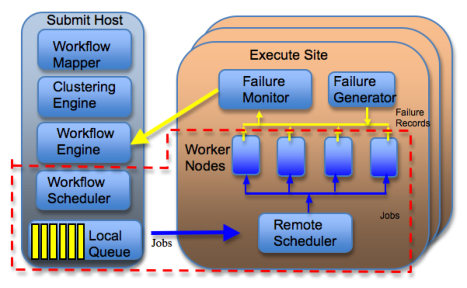
\includegraphics[width=0.7\textwidth]{figures/model/wfs_overview.pdf}
    \caption{WorkflowSim Overview. The area surrounded by red lines is supported by CloudSim}
    \label{fig:model_wfs_overview}
\end{figure}

However, an accurate simulation framework for scientific workflows is required to generate reasonable results, particularly considering that the overall system overhead \cite{Overhead2011} plays a significant role in the workflow’s runtime. 
%In heterogeneous distributed systems, workflows may experience different types of overheads, which are defined as the time of performing miscellaneous work other than executing users’ computational activities.  Since the causes of overheads differ, the overheads have diverse distributions and behaviors. For example, the time to run a post-script that checks the return status of a computation is usually a constant. However, queue delays incurred while tasks are waiting in a batch scheduling systems can vary widely. 
By classifying these workflow overheads in different layers and system components, our simulator can offer a more accurate result than simulators that do not include overheads in their system models.

What’s more, many researchers \cite{Zhang2004, Tang1990, Schroeder2006, Sahoo2004, Oppenheimer2002, Mcconnel} have emphasized the importance of fault tolerant design and concluded that the failure rates in modern distributed systems should not be neglected. A simulation with support for randomization and layered failures is supported in WorkflowSim to promote such studies. 

Finally, progress in workflow research also requires a general-purpose framework that can support widely accepted features of workflows and optimization techniques. Existing simulators such as CloudSim/GridSim \cite{Calheiros2011} fail to provide fine granularity simulations of workflows. For example, they lack the support of task clustering, which is a popular technique that merges small tasks into a large job to reduce task execution overheads. The simulation of task clustering requires two layers of execution model, on both task and job levels. It also requires a workflow-clustering engine that launches algorithms and heuristics to cluster tasks. Other techniques such as workflow partitioning and task retry are also ignored in these simulators. These features have been implemented in WorkflowSim. 

%To the best of our knowledge, none of the current distributed system simulators support these rich-features and techniques. In this section, we introduce our early work on simulating scientific workflows satisfying these requirements. We evaluate the performance of WorkflowSim with an example of task clustering. We further show that WorkflowSim is promising in providing an evaluation platform for research areas such as fault tolerant clustering and overhead robustness studies. 

\subsection{Components of WorkflowSim}

As Fig~\ref{fig:model_wfs_overview} shows, there are multiple layers of components involved in preparing and executing a workflow. Among them, Workflow Mapper, Workflow Engine, Workflow Scheduler and Job Execution have been introduced in last section. Below we introduce three components that have not been introduced. 
\begin{enumerate}

\item Clustering Engine

The Clustering Engine merges tasks into jobs so as to reduce the scheduling overheads. 

%\item Workflow Engine 

%The Workflow Engine manages jobs based on their dependencies to assure that a job may only be released when all of its parent jobs have completed successfully. The Workflow Engine will only release free jobs to the Scheduler. In the real execution we studied, we use DAGMan \cite{DAGMan} as the Workflow Engine. 
  
%\item Workflow Scheduler and Job Execution

%The Workflow Scheduler is used to match jobs to worker nodes based on the criteria selected by users (MaxMin \cite{Braun2001}, MinMin \cite{Blythe2005} , and many other heuristics). While CloudSim has already supported static scheduling algorithms, we added the support of dynamic workflow algorithms. For static algorithms, jobs are assigned to a worker node at the workflow planning stage. When the job reaches the remote scheduler, it will just wait until the assigned worker node is free. For dynamic algorithms, jobs are matched to a worker node in the remote scheduler whenever a worker node becomes idle. WorkflowSim relies on CloudSim to provide an accurate and reliable job-level execution model, such as time-shared model and space-shared model. However, WorkflowSim has introduced different layers of overheads and failures, which improves the accuracy of simulation. 

%\begin{figure}[h!]
%	\centering
 %   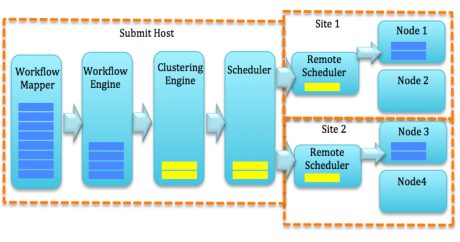
\includegraphics[width=0.7\textwidth]{figures/model/wfs_interaction.pdf}
  %  \caption{Interaction between components}
   % \label{fig:model_wfs_interaction}
%\end{figure}


%To associate and coordinate these layers, we adopted an event-based approach where each component maintains a message queue. Fig~\ref{fig:model_wfs_interaction} shows a simple configuration with two execution sites, of which each has two nodes. Each component maintains its own message queue and iteratively checks whether it can process one message. For example, at each iteration, the Clustering Engine checks whether it has received new tasks from the Workflow Engine and whether it should release new jobs to the Scheduler. When none of these components have any more messages in queue, the simulation is completed. 

%Based on our prior studies on workflow overheads, we add layered overhead to the workflow simulation. We have classified workflow overheads into five categories as follows. 
%\begin{enumerate}

%\item Workflow Engine Delay measures the time between when the last parent job of a job completes and the time when the job gets submitted to the local queue. In case of retries the value of the last retry is used for the calculation. Since we use a DAG model to represent workflows, the completion time of the last parent job means this job is released to the ready queue and is waiting for resources to be assigned to it. The workflow engine delay reflects the efficiency of a workflow engine (in our case DAGMan). 

%\item Queue Delay is defined as the time between the submission of a job by the workflow engine to the local queue and the time the local scheduler sees the job running (potentially on remote resources). This overhead reflects the efficiency of the workflow scheduler (e.g., Condor \cite{Frey2002}) to execute a job and the availability of resources for the execution of the job. In case of retries the value is the cumulative of all the retries.  
%\item Postscript Delay and Prescript Delay is the time taken to execute a lightweight script under some execution systems before and after the execution of a job. Prescripts are usually used to create directories for job execution. Postscripts examine the exit code of a job after the computational part of the job is done.
%\item Data Transfer Delay happens when data is transferred between nodes. It includes three different types of processes: staging data in, cleaning up, and staging data out. Stage-in jobs transfer input files from source sites to execution sites before the computation starts. Cleanup jobs delete intermediate data that is no longer needed by the remainder of the workflow. Stage-out jobs transfer workflow output data to archiving sites for storage and analysis.
%\item Clustering Delay measures the difference between the sum of the actual task runtime and the job runtime seen by the Workflow Scheduler. The cause of Clustering Delay is usually the use a job wrapper used to execute a clustered job. The wrapper takes some time to extract the list of tasks and to launch them. 
%\end{enumerate}                        

%Failures can occur at different times during the workflow execution. Consistent with the definition of tasks and job, we divide transient failures into two categories: task failure and job failure. If the transient failure affects the computation of a task (task failure), other tasks within the job do not necessarily fail. If the transient failure affects the clustered job (job failure), all of its tasks fail. We have added two components in response to the simulation of failures:
\item Failure Generator component is introduced to inject task/job failures at each execution site. After the execution of each job, Failure Generator randomly generates task/job failures based on the distribution and average failure rate that a user has specified. 
\item Failure Monitor collects failure records (e.g., resource id, job id, task id) and returns them to the workflow management system so that it can adjust the scheduling strategies dynamically. 
\end{enumerate}
We also modified other components to support fault tolerant optimization. In a failure-prone environment, there are several options to improve workflow performance. First, one can simply retry the entire job or only the failed part of this job when its computation is not successful. This functionality is added to the Workflow Scheduler, which checks the status of a job and takes action based on the strategies that a user selects. Furthermore, Reclustering is a technique that we have proposed \cite{Chen2012} that aims to adjust the task clustering strategy based on the detected failure rate. This functionality is added to the Workflow Engine. 

\subsection{Experiments and Validation}
We use task clustering as an example to illustrate the necessity of introducing overheads into workflow simulation. The goal was to compare the simulated overall runtime of workflows in case the information of job runtime and system overheads are known and extracted from prior traces. 
In this example, we collected real traces generated by the Pegasus Workflow Management System while executing workflows on FutureGrid \cite{FutureGrid}. We built an execution site with 20 worker nodes and we executed the Montage workflow five times in every single configuration of $k$, which is the maximum number of clustered jobs in a horizontal level. These five traces of workflow execution with the same $k$ is a training set or a validation set. 
%Partly illustrated by Figure 5, the results are stable enough to be used as a training set. 
We ran the Montage workflow with a size of 8-degree squares of sky. The workflow has 10,422 tasks and 57GB of overall data. We tried different k from 20 to 100, leaving us 5 groups of data sets with each group having 5 workflow traces. 
First of all, we adopt a simple approach that selects a training set to train WorkflowSim and then use the same training set as validation set to compare the predicted overall runtime and the real overall runtime in the traces. We define accuracy in this section as the ratio between the predicted overall runtime and the real overall runtime:
\begin{equation} \label{eq:model_wfs_accuracy}
Accuracy=\frac{Predicted~Overall~Runtime}{Real~Overall~Runtime}
\end{equation}
 \begin{figure}[h!]
	\centering
    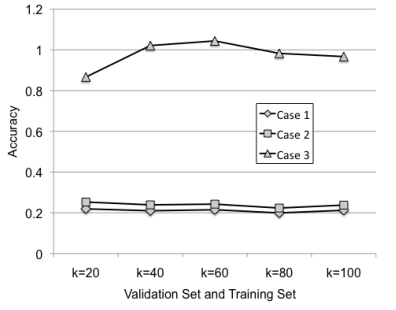
\includegraphics[width=0.6\textwidth]{figures/model/wfs_levels.pdf}
    \caption{Performance of WorkflowSim with different support levels}
    \label{fig:model_wfs_levels}
\end{figure} 
 
Performance of WorkflowSim with different support levels. 
To train WorkflowSim, from the traces of workflow execution (training sets), we extracted information about job runtime and overheads, such as average/distribution and, for example, whether it has a cyclic increase. We then added these parameters into the generation of system overheads and simulated them as close as possible to the real cases. Here, we do not discuss the randomization or distribution of job runtime since we rely on CloudSim to provide a convincing model of job execution.

To present an explicit comparison, we simulated the cases using WorkflowSim that has no consideration of workflow dependencies or overheads (Case 1), WorkflowSim with Workflow Engine that has considered the influence of dependencies but ignored overheads (Case 2), and WorkflowSim, that has covered both aspects (Case 3). Intuitively speaking, we expect that the order of the accuracy of them should be Case 3 $>$ Case 2 $>$ Case 1. 

% \begin{figure}[h!]
%	\centering
%    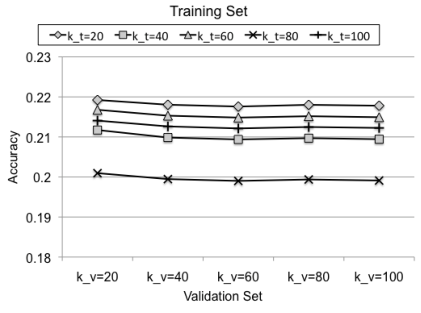
\includegraphics[width=0.6\textwidth]{figures/model/wfs_case1.pdf}
%    \caption{Performance of WorkflowSim of Case 1 (No workflow engine, or overhead support)}
 %   \label{fig:model_wfs_case1}
%\end{figure} 
 
%\begin{figure}[h!]
%	\centering
 %   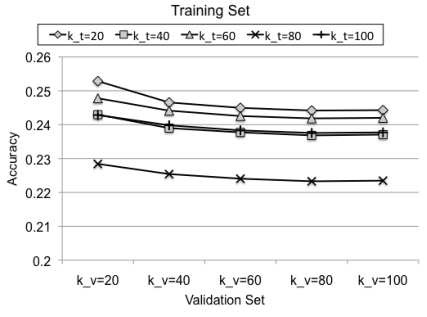
\includegraphics[width=0.6\textwidth]{figures/model/wfs_case2.pdf}
  %  \caption{Performance of WorkflowSim of Case 2 (No overhead support)}
    %\label{fig:model_wfs_case2}
%\end{figure} 

Fig~\ref{fig:model_wfs_levels} shows the performance of WorkflowSim with different support levels is consistent to our expectation. The accuracy of Case 3 is quite close to but not equal to 1.0 in most points. The reason is that to simulate workflows, WorkflowSim has to simplify models with a few parameters, such as the average value and the distribution type. It is not efficient to recur every overhead as is present in the real traces. It is also impossible to do since the traces within the same training set may have much variance. Fig~\ref{fig:model_wfs_levels} also shows that the accuracy of both Case 1 and Case 2 are much lower than Case 3. The reason why Case 1 does not give an exact result is that it ignores both dependencies and multiple layers of overheads. By ignoring data dependencies, it releases tasks that are not supposed to run since their parents have not completed (a real workflow system should never do that) and thereby reducing the overall runtime. At the same time, it executes jobs/tasks irrespective of the actual overheads, which further reduces the simulated overall runtime. In Case 2, with the help of Workflow Engine, WorkflowSim is able to control the release of tasks and thereby the simulated overall runtime is closer to the real traces. However, since it has ignored most overheads, jobs are completed and returned earlier than that in real traces. The low accuracy of Case 1 and Case 2 confirms the necessity of introducing overhead design into our simulator. 

%To further evaluate our task/job model and the performance of WorkflowSim, we adopted a cross-validation approach in which we picked up one group of data set (e.g., $k_t=20$) as input traces/training sets and simulated all the validation sets with $k_v=20$ to 100. To make it clear, we use $k_t$ to indicate the $k$ for a training set and $k_v$ for a validation set. Then we compare the accuracy in Fig~\ref{fig:model_wfs_case1}, Fig~\ref{fig:model_wfs_case2} and Fig~\ref{fig:model_wfs_case3} respectively. 
 
%\begin{figure}[h!]
%	\centering
%    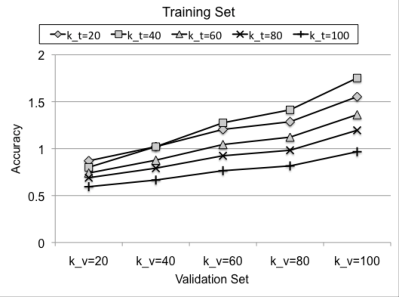
\includegraphics[width=0.6\textwidth]{figures/model/wfs_case3.pdf}
%   \caption{Performance of WorkflowSim of Case 3 (all features are enabled).}
%  \label{fig:model_wfs_case3}
%\end{figure} 

%Fig~\ref{fig:model_wfs_case1} and Fig~\ref{fig:model_wfs_case2} show similar conclusion as in Fig~\ref{fig:model_wfs_levels} and the accuracy of Case 2 and Case 1 are not sensitive to the task clustering. The reason is that Case 1 has no support of data dependencies, where jobs are all submitted at the beginning of workflow execution.  Case 2 has no support of system overhead and thereby task clustering does not improve the overall runtime much. Fig~\ref{fig:model_wfs_case3} shows the simulated results of WorkflowSim, which has considered both layered overhead and data dependencies. Although the accuracy is closer to 1.0, it still does not guarantee a 100\% accuracy in some cases. Particularly when we use a training set with a smaller k (e.g., $k_t=20$) to simulate the case with larger k (e.g., $k_v=100$), the accuracy suffers (accuracy=1.8). The reason is that the average Clustering Delay in the case of $k=20$ is much larger than that of other cases (as shown in Fig~\ref{fig:model_wfs_case2}), and thereby it is still larger than the predicted one using an inverse proportion function. Using such a large Clustering Delay to simulate the case with many clustered jobs ($k_v$ is large) would extend the predicted overall runtime of workflow. Our model has simplified and classified the distribution of overheads based on the horizontal level of tasks but we still need to further study the overhead distribution in accordance to different clustering strategies. However, a complex model may limit its general usage.  

%\subsection{Applications}

%With the features introduced in last section, we are able to carry out research studies such as evaluation of overhead robustness of DAG scheduling heuristics

%\begin{figure}[h!]
%	\centering
%    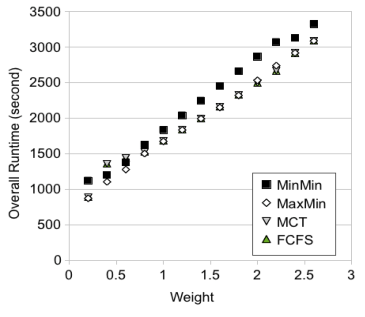
\includegraphics[width=0.6\textwidth]{figures/model/wfs_queue_delay.pdf}
%    \caption{Influence of Queue Delay. The duration of overheads are multiplied by the weights.}
%   \label{fig:model_wfs_queue_delay}
%\end{figure} 

%With the emergence of distributed heterogeneous systems, such as grids and clouds, and applications such as  large scale of workflows with  complex data dependencies, significant overheads can be incurred during workflow execution. Most of the existing DAG scheduling heuristics underestimate or even ignore the influence of workflow overheads. In such a distributed environment, a carefully crafted schedule based on deterministic and static information may fail to provide a sufficient solution. In this study, we analyze the overhead robustness of multiple static and dynamic DAG scheduling heuristics. Overhead robustness describes the influence of overheads on the workflow runtime. We investigate whether the dynamic change in workflow overheads influences the overall runtime of workflows. The reason why we are interested in this study is that in reality, system overheads are difficult to estimate or track. Existing heuristics and algorithms may have different sensitivity to the dynamic change of system overhead or the inaccurate estimation of them. Analyzing their performance in terms of the change of overheads can offer us a unique aspect of their robustness in real systems and suggest the direction of designing new heuristics or algorithms.

%\begin{figure}[h!]
%	\centering
%    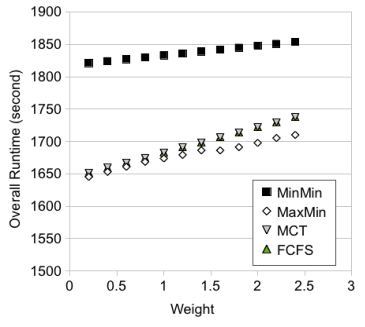
\includegraphics[width=0.6\textwidth]{figures/model/wfs_engine_delay.pdf}
%    \caption{Influence of Workflow Engine Delay}
%    \label{fig:model_wfs_engine_delay}
%\end{figure} 
%\begin{figure}[h!]
%	\centering
%    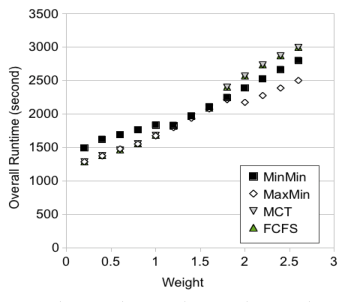
\includegraphics[width=0.6\textwidth]{figures/model/wfs_clustering_delay.pdf}
%   \caption{Influence of Clustering Delay}
%    \label{fig:model_wfs_clustering_delay}
%\end{figure} 


%In this experiment, we doubled the computation capabilities of half of the available resources so as to create an environment where heuristics and algorithms can select their allocated resources to execute workflow jobs.  We varied the duration of overheads by multiplying them with a weight that ranges from 0.2 to 2.5 in our experiment. The original workflow has the weight is 1.0. We evaluated the performance of four heuristics with the same Montage workflow used in Section VI: 
%\begin{enumerate}
%\item FCFS: First Come First Serve is the basic version of scheduling algorithm used in our simulator. It assigns each job, in the arriving order to the next available resources, regardless of the jobs’ expected completion time on that worker node. If there are multiple resources available, it randomly chooses one as the candidate. 
%\item MCT: Minimum Completion Time \cite{Braun2001} assigns each job in an arbitrary order to the available resource with the best expected completion time of that job. 
%\item MinMin: The MinMin \cite{Blythe2005} heuristic begins with a set of all free jobs and then sorts them by the order of completion time. The job with the minimum completion time is selected and assigned to the corresponding resource.  Then, the newly mapped job is submitted to the queue and the process repeats until all free jobs are scheduled. The intuition of MinMin is to create a local optimal path so as to reduce the overall runtime. 
%\item MaxMin: Similar to MinMin, but MaxMin \cite{Braun2001} picks up the job with the maximum completion time and assigns it to its best available resource. The intuition of MaxMin is to avoid penalty from long running jobs. 
%\end{enumerate}

%Experiments show that overheads have significant influence on the overall runtime and they have shown different behaviors. Fig~\ref{fig:model_wfs_queue_delay} and Fig~\ref{fig:model_wfs_engine_delay} show the influence of Queue Delay and Workflow Engine Delay respectively. Consistent with our expectation, MinMin performs worst compared to the other three methods since it assigns the best resources to small jobs while longer jobs have to wait and suffer overhead. MaxMin performs better than MCT and FCFS slightly because it tends to assign longer jobs to better resources and thereby reduces the overall runtime. Fig~\ref{fig:model_wfs_clustering_delay} shows that when the weight of Clustering Delay is lower than 1.0, MCT and FCFS perform better than MinMin. However, when the weight of Clustering Delay is larger than 2, MinMin performs better than the other two. The reason is probably because Clustering Delay only occurs to clustered jobs and in Montage these levels have better parallelism than other levels that have only non-clustered jobs. Increasing Clustering Delay thereby offers MinMin a chance to enhance its influence on the overall workflow execution. Therefore, in such an environment, the selection of heuristics is not sensitive to the estimation error of the Queue Delay or Workflow Engine Delay because the overall runtime increases at the same speed. However, the estimation error of the Clustering Delay can change the heuristics’ relative performance. 
%Only used in defense
%\subsection{Conclusion}
%In this section, we have introduced a novel workflow simulator WorkflowSim to assist researchers to evaluate their workflow optimization techniques with better accuracy and wider support than existing solutions. By comparing the results of real traces and simulation, we have validated our simulator and concluded that it is necessary to consider multiple layers of overheads and failures. In the future, we would also define more types of failures, such as the Job Submit Failure that simulates the case when a job is not successfully submitted due to a problem in workflow scheduler or a network issue between it and remote scheduler. We also plan to incorporate more workflow techniques (such as workflow partitioning) into our simulator. We will evaluate the influence of overheads in other workflow metrics besides overall runtime, for example, resource utility. 

\chapter{Data Aware Workflow Partitioning}
\label{chap:partitioning}

In this chapter, we introduce our work on data aware workflow partitioning that divides large-scale workflows into several sub-workflows that are fit for execution within a single execution site. Three widely used workflows have been used to evaluate the effectiveness of out methods and the experiments show an runtime improvement of up to 48.1\%. 


\section{Motivation}

Data movement between tasks in scientific workflows has received less attention compared to task execution. Often the staging of data between tasks is either assumed or the time delay in data transfer is considered to be negligible compared to task execution, which is not true in many cases, especially in data-intensive applications. In this chapter, we take the data transfer into consideration and propose to partition large workflows into several sub-workflows where each sub-workflows can be executed within one execution site. 

The motivation behind workflow partitioning starts from a common scenario where a researcher at a research institution typically has access to several research clusters, each of which may consist of a small number of nodes. The nodes in one cluster may be very different from those in another cluster in terms of file system, execution environment, and security systems. For example, we have access to FutureGrid \cite{Fox2013FutureGrid}, Teragrid/XSEDE \cite{TeraGrid}  and Amazon EC2 \cite{AmazonAWS} but each cluster imposes a limit on the resources, such as the maximum number of nodes a user can allocate at one time or the maximum storage. If these isolated clusters can work together, they collectively become more powerful.

Additionally, the input dataset could be very large and widely distributed across multiple clusters. Data-intensive workflows require significant amount of storage and computation and therefore the storage system becomes a bottleneck. For these workflows, we need to use multiple execution sites and consider their available storage. For example, the entire CyberShake earthquake science workflow has 16,000 sub-workflows and each sub-workflow has more than 24,000 individual jobs and requires 58 GB of data. In this chapter, we assume we have Condor installed at the execution sites. A Condor pool can be either a physical cluster or a virtual cluster. 

The first benefit of workflow partitioning is that this approach reduces the complexity of workflow mapping. For example, the entire CyberShake workflow has more than $3.8\times 10^8$ tasks, which is a significant load for workflow management tools to maintain or schedule. In contrast, each sub-workflow has 24,000 tasks, which is acceptable for workflow management tools. A sub-workflow is a workflow and also a job of a higher-level workflow. What is more, workflow partitioning provides \textbf{a fine granularity adjustment of workflow activities} so that each sub-workflow can be adequate for one execution site. In the end, workflow partitioning allows us to migrate or retry sub-workflows efficiently. The overall workflow can be partitioned into sub-workflows and each sub-workflow can to be executed in different execution environments such as a hybrid platform of Condor/DAGMan \cite{DAGMan} and MPI/DAGMan \cite{Rynge2012}) while the traditional task clustering technique requires all the tasks can be executed in the same execution environment. 


%should fix it

 
%There are large differences in I/O speeds from local disk storage to wide area networks. Feeding a large dataset repeatedly to re- mote computing resources becomes the bottleneck. When mapping such data-intensive tasks to compute resources, scheduling mechanisms need not only take into account the execution time of the tasks, but also the overheads of staging the dataset. To scale up such tasks, there are tradeoffs to be made, such as determining whether to bring data to computation or bring computation to data, or even regenerate data on-the-fly.

%While scheduling workflows there exists more than one task that can be scheduled independently of one another. Since our workflows are data intensive in nature, the transfer time are dominant as compared to the computation time. This gives rise to the possibility that majority of tasks are assigned to a single or only few compute resources. This occurs only when tasks have more than one input file in common and these files are only available from selected few resources. In such cases, grouping these tasks to form a batch task and submitting to a resource reduces data-transfer time.

%\section{Related Work}
%For convenience and cost-related reasons, scientists execute scientific workflows \cite{Bharathi2008, Rubing2005} in distributed large-scale computational environments such as multi-cluster grids, that is, grids comprising multiple independent execution sites. Topcuoglu \cite{Topcuoglu2002} presented a classification of widely used task scheduling approaches. Such scheduling solutions, however, cannot be applied directly to multi-cluster grids. First, the data transfer delay between multiple execution sites is more significant than that within an execution site and thus a hierarchical view of data transfer is necessary. Second, they do not consider the resource availability experienced in grids, which also makes accurate predictions of computation and communication costs difficult. Sonmez \cite{Sonmez2010} extended the traditional scheduling problem to multiple workflows on multi-cluster grids and presented a performance of a wide range of dynamic workflow scheduling policies in multi-cluster grids. Duan \cite{Rubing2005} and Wieczorek \cite{Wieczorek2005} have discussed the scheduling and partitioning scientific workflows in dynamic grids with challenges such as a broad set of unpredictable overheads and possible failures. Duan \cite{Rubing2005} then developed a distributed service-oriented Enactment Engine with a master-slave architecture for de-centralized coordination of scientific workflows. Kumar \cite{Kumar2002} proposed the use of graph partitioning for partition the resources of a distributed system, but not the workflow DAG, which means the resources are provisioned into different execution sites but the workflows are not partitioned at all. Dong \cite{Dong2007} and Kalayci \cite{Kalayci2010} have discussed the use of graph partitioning algorithms for the workflow DAG according to features of the workflow itself and the status of selected available resource clusters. Our work focuses on the workflow partitioning problem with resource constraints. Compared to Dong \cite{Dong2007} and Kalayci \cite{Kalayci2010}, we extend their work to estimate the overall runtime of sub-workflows and then schedule these sub-workflows based on the estimates. 

%Yu \cite{Yu2005a} classified existing automated data transfer strategies utilized among tasks in workflows, namely centralized, mediated, and peer-to-peer. A centralized approach utilizes a central point for data transmission. This solution is not scalable, and occurs in systems where the time for data transfers is much smaller than computations. Taverna \cite{Oinn2004} typically utilizes a centralized data transfer, due to the characteristics of the problems it tackles. In a mediated strategy the locations of the intermediate data are managed by a distributed data management system. Finally, a peer-to-peer approach transfers data directly between processing nodes. The direct transmissions of peer-to-peer approaches reduce both transmission time and the bottleneck problem caused by the centralized and mediated approaches. Thus, they are suitable for large-scale intermediate data transfer. For simplicity, we use centralized data services but our work can be easily extended to the peer-to-peer approach with modifications. 

%The Pegasus workflow system [7] has also dealt with data-intensive workflows and has incorporated both mediated and peer-to-peer transfers. In the mediated approach, Pegasus utilises a data replica catalogue that stores the intermediate data generated, so data can be subsequently retrieved rather than recomputed again. Workflow performance speedup has also been a matter of study in Pegasus, and abstract workflow specifications go through a process of clustering (grouping of small tasks) and partitioning which helps the meta-scheduler to optimise the execution time. A similar approach was followed in \cite{Rubing2005} with further optimisation at runtime by adapting to the dynamically changing state of underlying resources. However, none of these approaches makes an effective usage of both network bandwidth and buffer/storage of files.

%Park et al. \cite{Humphrey2008} limits the amount of parallel data transfer to avoid overloading supporting services such as data servers, which is called data throttling. Throttling is especially useful for unbalanced workflows in which one task might be idle while waiting for data to arrive. However, as discussed in \cite{Humphrey2008}, data throttling has an impact on the overall workflow performance depending on the ratio between computational and data transfer tasks. Therefore, performance analysis is necessary after the profiling of data transfers so that the relationship between computation and data transfers can be identified more explicitly. Rodríguez \cite{Rodríguez2012} proposed an automated and trace-based workflow structural analysis method for DAGs. Files transfers are accomplished as fast as the network bandwidth allows, and once transferred, the files are buffered/stored at their destination. To improve the use of network bandwidth and buffer/storage within a workflow, they adjusted the speeds of some data transfers and assured that tasks have all their input data arriving at the same time. Compared to our work, data throttling has a limit in performance gain by the amount of data transfer that can be reduced, while our partitioning approach can improve the overall workflow runtime and resource usage. 

%Data Placement techniques try to strategically manage placement of data before or during the execution of a workflow. Kosar et al. \cite{Kosar2004} presented Stork, a scheduler for data placement activities on grids and proposed to make data placement activities as first class citizens in the Grid. In Stork, data placement is a job and is decoupled from computational jobs. Amer et al. \cite{Amer2012} studied the relationship between data placement services and workflow management systems for data-intensive applications. They proposed an asynchronous mode of data placement in which data placement operations are performed as data sets become available and according to the policies of the virtual organization and not according to the directives of the workflow management system (WMS). The WMS can however assist the placement services with the placement of data based on information collected during task executions and data transfers. Shankar \cite{Shankar2007} presented an architecture for Condor in which the input, output and executable files of jobs are cached on the local disks of the machines in a cluster. Caching can reduce the amount of pipelines and batch I/O that is transferred across the network. This in turn significantly reduces the response time for workflows with data-intensive workloads. In contrast, we mainly focus on the workflow partitioning problem but our work can be extended to consider the data placement strategies they have proposed in the future. 

%With caching enabled, data-intensive applications can reuse the files and also be able to compare between old and new versions of the file. They presented a planning algorithm that takes into account the location of cached data together with data dependencies between jobs in a workflow. Their planning algorithm produces a schedule by comparing the time saved by running jobs in parallel with the time taken for transferring data when dependent jobs are scheduled on different machines. 

%Data replication is a common way to increase the availability of data and implicit replication also occurs when scientists download and share the data for experimental purposes, in contrast to explicit replications done by workflow systems. Ranganathan  \cite{Ranganathan2001} conducted extensive studies for identifying dynamic data or task replication strategies, asynchronous data placement and job and data scheduling algorithms for Data Grids. They concluded through simulations of independent jobs that scheduling jobs to locations that contain the data they need and asynchronously replicating popular data sets to remote sites can improve the performance. We do not address data replication in our current work but it is worthy of further investigation of how data replication can improve the performance of workflow partitioning. 

%Their replication process at each site periodically generates new replicas for popular datasets. For dataset placement scheduler they define three algorithms: Data- DoNothing- no active replication takes place, DataRandom- popular datasets are replicated to a random site on the Grid, DataLeastLoaded- popular datasets are replicated to a least loaded neighboring site. 

%In data-intensive applications, replication may or may not be feasible. 

\section{Approach}

To efficiently partition workflows, we proposed a three-phase scheduling approach integrated with the Pegasus Workflow Management System to partition, estimate, and schedule workflows onto distributed resources. Our contribution includes three heuristics to partition workflows respecting storage constraints and internal job parallelism. We utilize three methods to estimate and compare runtime of sub-workflows and then we schedule them based on two commonly used algorithms (MinMin and HEFT).  

\begin{figure}[lh!]
	\centering
    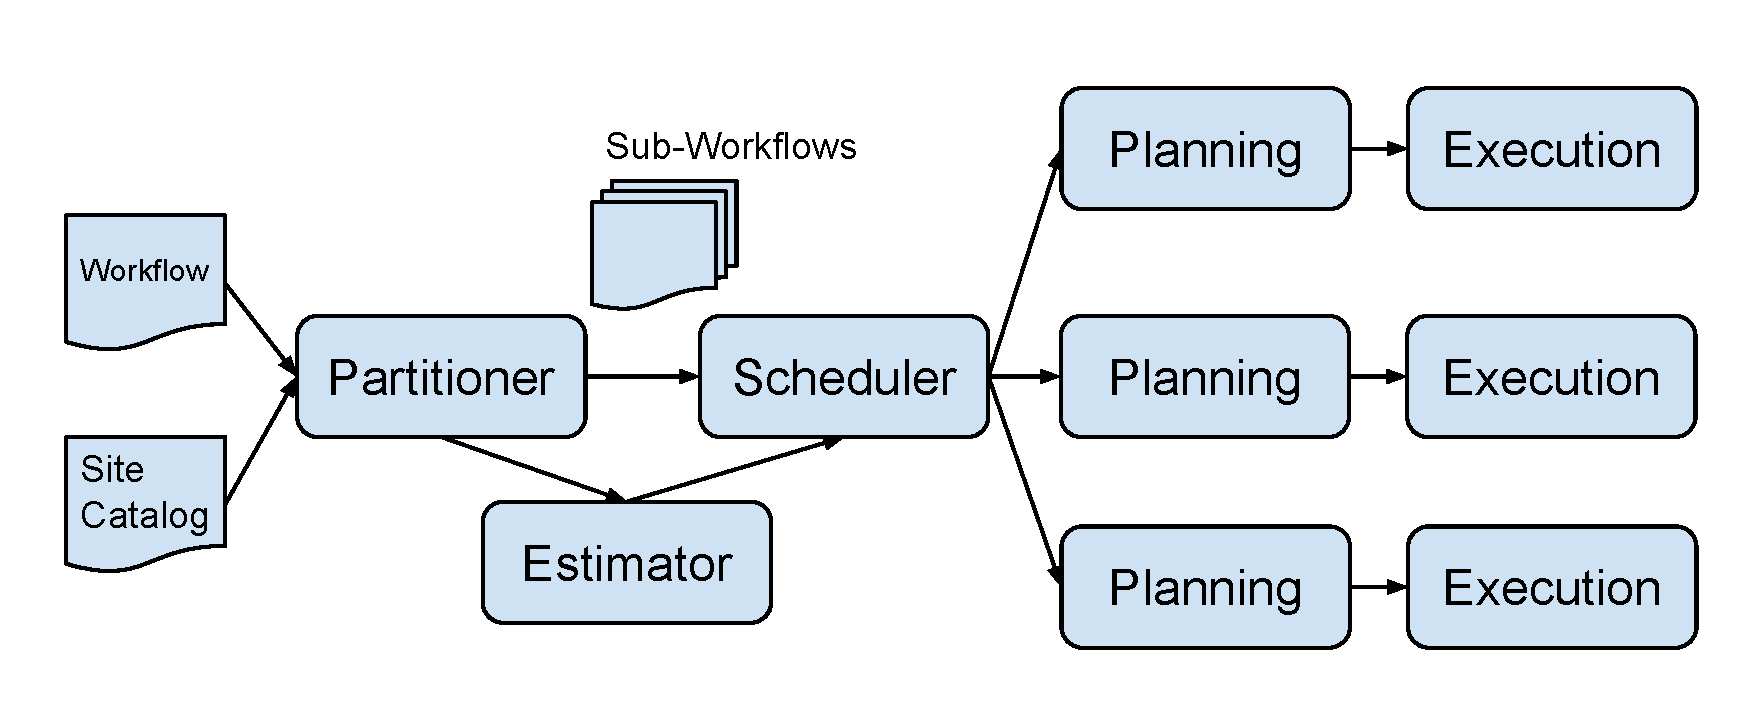
\includegraphics[width=0.8\textwidth]{figures/partitioning/partitioning_steps.pdf}
    \caption{The steps to partition and schedule a workflow}
    \label{fig:partitioning_steps}
\end{figure}
\begin{figure}[lh!]
	\centering
    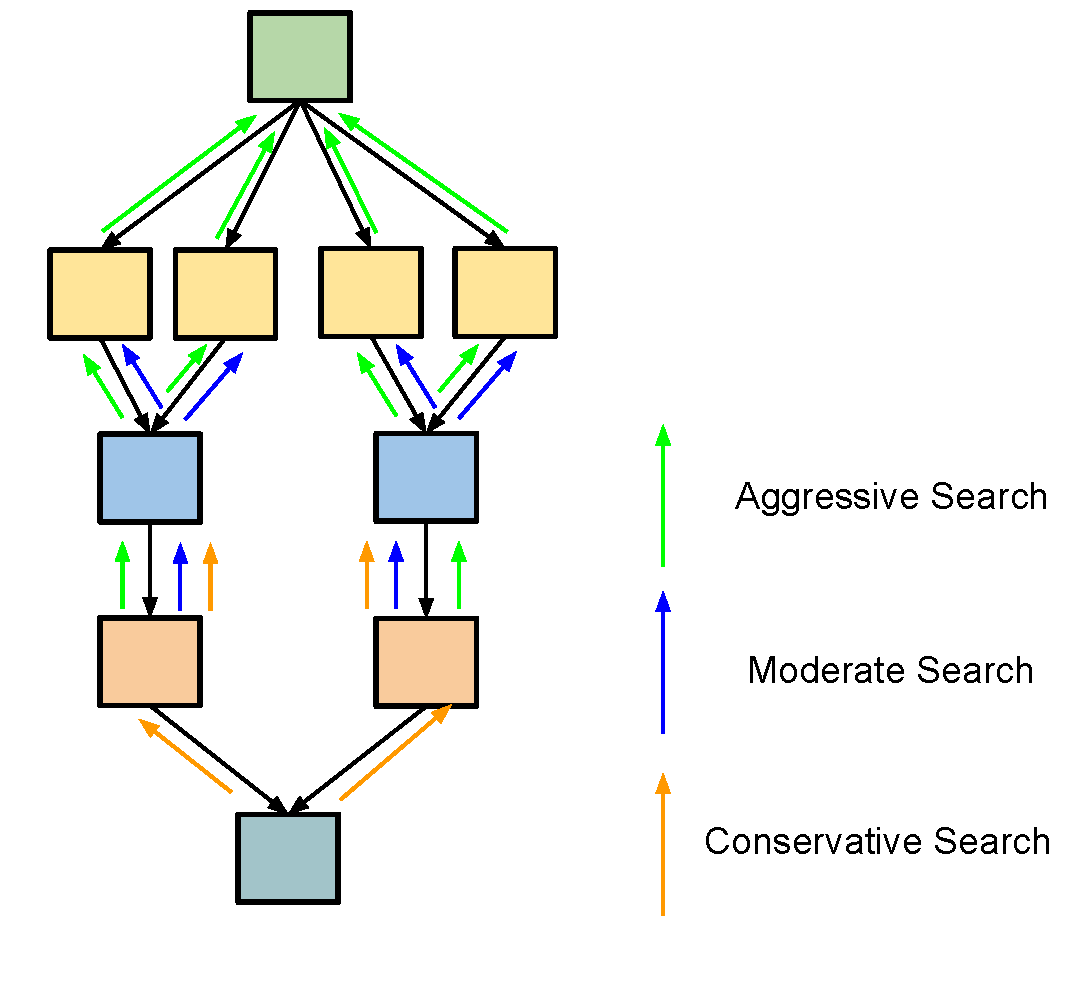
\includegraphics[width=0.7\textwidth]{figures/partitioning/three_steps.pdf}
    \caption{Three Steps of Search}
    \label{fig:three_steps}
\end{figure}
\begin{figure}[lh!]
	\centering
    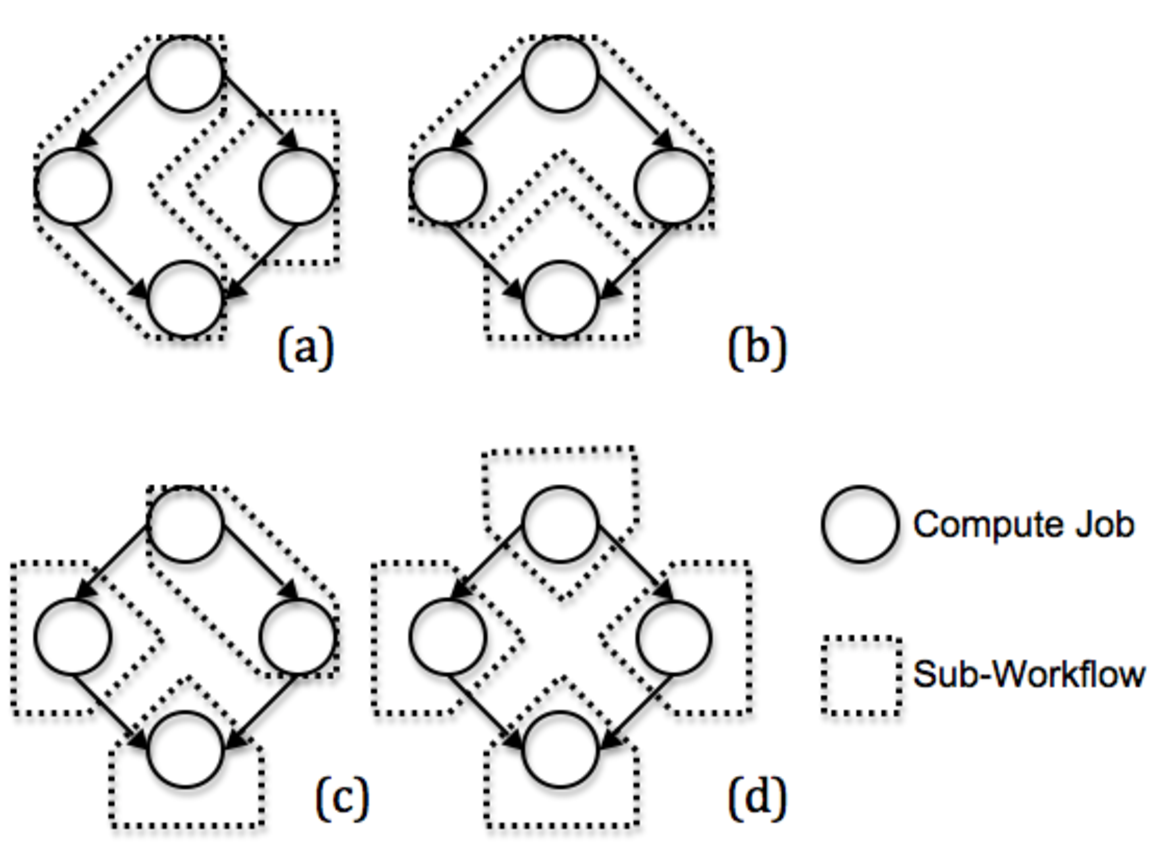
\includegraphics[width=0.9\textwidth]{figures/partitioning/four_partitioning.pdf}
    \caption{Four Partitioning Methods}
    \label{fig:four_partitioning}
\end{figure}
Our approach (see Figure~\ref{fig:partitioning_steps}) has three phases: partition, estimate and schedule. The partitioner takes the original workflow and site catalog as input, and outputs various sub-workflows that respect the storage constraints—this means that the data requirements of a sub-workflow are within the data storage limit of a site. The site catalog provides information about the available resources. The estimator provides the runtime estimation of the sub-workflows and supports three estimation methods. The scheduler maps these sub-workflows to resources considering storage requirement and runtime estimation. The scheduler supports two commonly used algorithms. We first guarantee to find a valid mapping of sub-workflows satisfying storage constraints. Then we optimize performance based on these generated sub-workflows and schedule them to appropriate execution sites if runtime information for individual jobs is already known. If not, a static scheduler maps them to resources merely based on storage requirements. 

The major challenge in partitioning workflows is to avoid cross dependency, which is a chain of dependencies that forms a cycle in graph (in this case cycles between sub-workflows). With cross dependencies, workflows are not able to proceed since they form a deadlock loop. For a simple workflow depicted in Figure~\ref{fig:four_partitioning}, we show the result of four different partitioning. Partitioning (a) does not work in practice since it has a deadlock loop. Partitioning (c) is valid but not efficient compared to Partitioning (b) or (d) that have more parallelism. 

Usually jobs that have parent-child relationships share a lot of data since they have data dependencies. It’s reasonable to schedule such jobs into the same partition to avoid extra data transfer and also to reduce the overall runtime. Thus, we propose Heuristic I to find a group of parents and children. Our heuristic only checks three particular types of nodes: the fan-out job, the fan-in job, and the parents of the fan-in job and search for the potential candidate jobs that have parent-child relationships between them. The check operation means checking whether one particular job and its potential candidate jobs can be added to a sub-workflow while respecting storage constraints. Thus, our algorithm reduces the time complexity of check operations by n folds, while n is the average depth of the fan-in-fan-out structure. The check operation takes more time than the search operation since the calculation of data usage needs to check all the data allocated to a site and see if there is data overlap. Similar to \cite{Topcuoglu2002}, the algorithm starts from the sink job and proceeds upward. 

To search for the potential candidate jobs that have parent-child relationships, the partitioner tries three steps of searches. For a fan-in job, it first checks if it’s possible to add the whole fan structure into the sub-workflow (aggressive search). If not, similar to Figure~\ref{fig:four_partitioning}(d), a cut is issued between this fan-in job and its parents to avoid cross dependencies and increase parallelism. Then a less aggressive search is performed on its parent jobs, which includes all of its predecessors until the search reaches a fan-out job. If the partition is still too large, a conservative search is performed, which includes all of its predecessors until the search reaches a fan-in job or a fan-out job. Figure~\ref{fig:three_steps} depicts an example of three steps of search while the workflow in it has an average depth of 4. Pseudo-code of Heuristic I is depicted in Algorithm~\ref{alg:parworkflow} .

%The partitioner starts by picking an execution site from site catalog and forming a sub-workflow with the heuristic above. Users must specify the order of execution sites to be picked. If the execution site does not have sufficient storage to host any more jobs, a new execution site is selected and so on. For the dependencies between jobs across multiple sub-workflows, they form the new dependencies between sub-workflows and are added to the final graph. The partitioner guarantees to satisfy storage constraints since in each step it assures the size of all sub-workflows assigned to a site is smaller than its storage constraint. 

We propose two other heuristics to solve the problem of cross dependency. The motivation for Heuristic II is that Partitioning (c) in Figure~\ref{fig:four_partitioning} is able to solve the problem. The motivation for Heuristic III is an observation that partitioning a fan structure into multiple horizontal levels is able to solve the problem. Heuristic II adds a job to a sub-workflow if all of its unscheduled children can be added to that sub-workflow without causing cross dependencies or exceed the storage constraint. Heuristic III adds a job to a sub-workflow if two conditions are met: 
\begin{enumerate}
\item For a job with multiple children, each child has already been scheduled.
\item After adding this job to the sub-workflow, the data size does not exceed the storage constraint.  
\end{enumerate}

To optimize the workflow performance, runtime estimation for sub-workflows is required assuming runtime information for each job is already known. We provide three methods. 
\begin{enumerate}
\item Critical Path is defined as the longest depth of the sub-workflow weighted by the runtime of each job. 
\item Average CPU Time is the quotient of cumulative CPU time of all jobs divided by the number of available resources (it’s the number of Condor slots in our experiments, which is also the maximum number of Condor jobs that can be run on one machine). \item The HEFT estimator uses the calculated earliest finish time of the last sink job as makespan of sub-workflows assuming that we use HEFT to schedule sub-workflows. 
\end{enumerate}

\begin{algorithm}[h!]
\caption{Workflow Partitioning algorithm}
\label{alg:parworkflow}
\begin{algorithmic}[1]
\Require $G$: workflow; $SL[index]$: site list, which stores all information about a compute site
\Ensure Create a subworkflow list $SWL$ that does not exceed storage constraints
\Procedure{ParWorkflow}{$G, SL$}
   \State $index\gets 0$
   \State $Q\gets$ new Queue()
   \State Add the sink job of $G$ to $Q$
   \State $S\gets$ new subworkflow()
   \While{$Q$ is not empty}
      \State $j\gets$ the last job in $Q$
      \State \Call{Aggressive-Search}{$j$} \Comment{for fan-in job}
      \State $C\gets$ the list of potential candidate jobs to be added to $S$ in $SL[index]$
      \State $P\gets$ the list of parents of all candidates
      \State $D\gets$ the data size in $SL[index]$ with $C$
      \If{$D>$ storage constraint of $SL[index]$}
         \State \Call{Less-Aggressive-Search}{j}, update $C,P,D$
      
      \If{$D>$ storage constraint of $SL[index]$}
         \State \Call{Conservative-Search}{j}, update $C,P,D$
      \EndIf
      \EndIf
	\State ...\Comment{for other jobs}
         \If{$S$ causes cross dependency in $SL[index]$}
         \State$S=$ new subworkflow()
      \EndIf
     \State Add all jobs in $C$ to $S$
     \State Add all jobs in $P$ to the head of $Q$
     \State Add $S$ to $SWL[index]$
     \If{$S$ has no enough space left}
         \State $index++$
      \EndIf
   \State ... \Comment{for other situations}
   \State Remove $j$ from $Q$
   \EndWhile
   \State \textbf{return }$SWL$

\EndProcedure
\end{algorithmic}
\end{algorithm}


The scheduler selects appropriate resources for the sub-workflows satisfying the storage constraints and optimizes the runtime performance. Since the partitioning step has already guaranteed that there is a valid mapping, this step is called re-ordering or post-scheduling. We select HEFT\cite{Topcuoglu2002} and MinMin\cite{Blythe2005}, which represent global and local optimizations respectively. But there are two differences compared to their original versions. First, the data transfer cost within a sub-workflow is ignored since we use a shared file system in our experiments. Second, the data constraints must be satisfied for each sub-workflow. 
The scheduler selects an optimal set of resources in terms of available Condor slots since it’s the major factor influencing the performance. This work can be easily extended to considering more factors. Although some more comprehensive algorithms can be adopted, HEFT or MinMin are able to find an optimal schedule in terms that the sub-workflows are already generated since the number of sub-workflows has been greatly reduced compared to the number of individual jobs.

\section{Experiments and Discussion}
In order to quickly deploy and reconfigure computational resources, we use a private cloud computing resource running Eucalyptus \cite{Nurmi2008b}. Eucalyptus is an infrastructure software that provides on-demand access to Virtual Machine (VM) resources. In all the experiments, each VM has 4 CPU cores, 2 Condor slots, 4GB RAM and has a shared file system mounted to make sure data staged into a site is accessible to all compute nodes. In the initial experiments we build up four clusters, each with 4 VMs, 8 Condor slots. In the last experiment of site selection, the four virtual clusters are reconfigured and each cluster has 4, 8, 10 and 10 Condor slots respectively. The submit host that performs workflow planning and which sends jobs to the execution sites is a Linux 2.6 machine equipped with 8GB RAM and an Intel 2.66GHz Quad CPUs. We use Pegasus to plan the workflows and then submit them to Condor DAGMan \cite{DAGMan}, which provides the workflow execution engine. Each execution site contains a Condor pool and a head node visible to the network. 

\begin{figure}[h!]
	\centering
    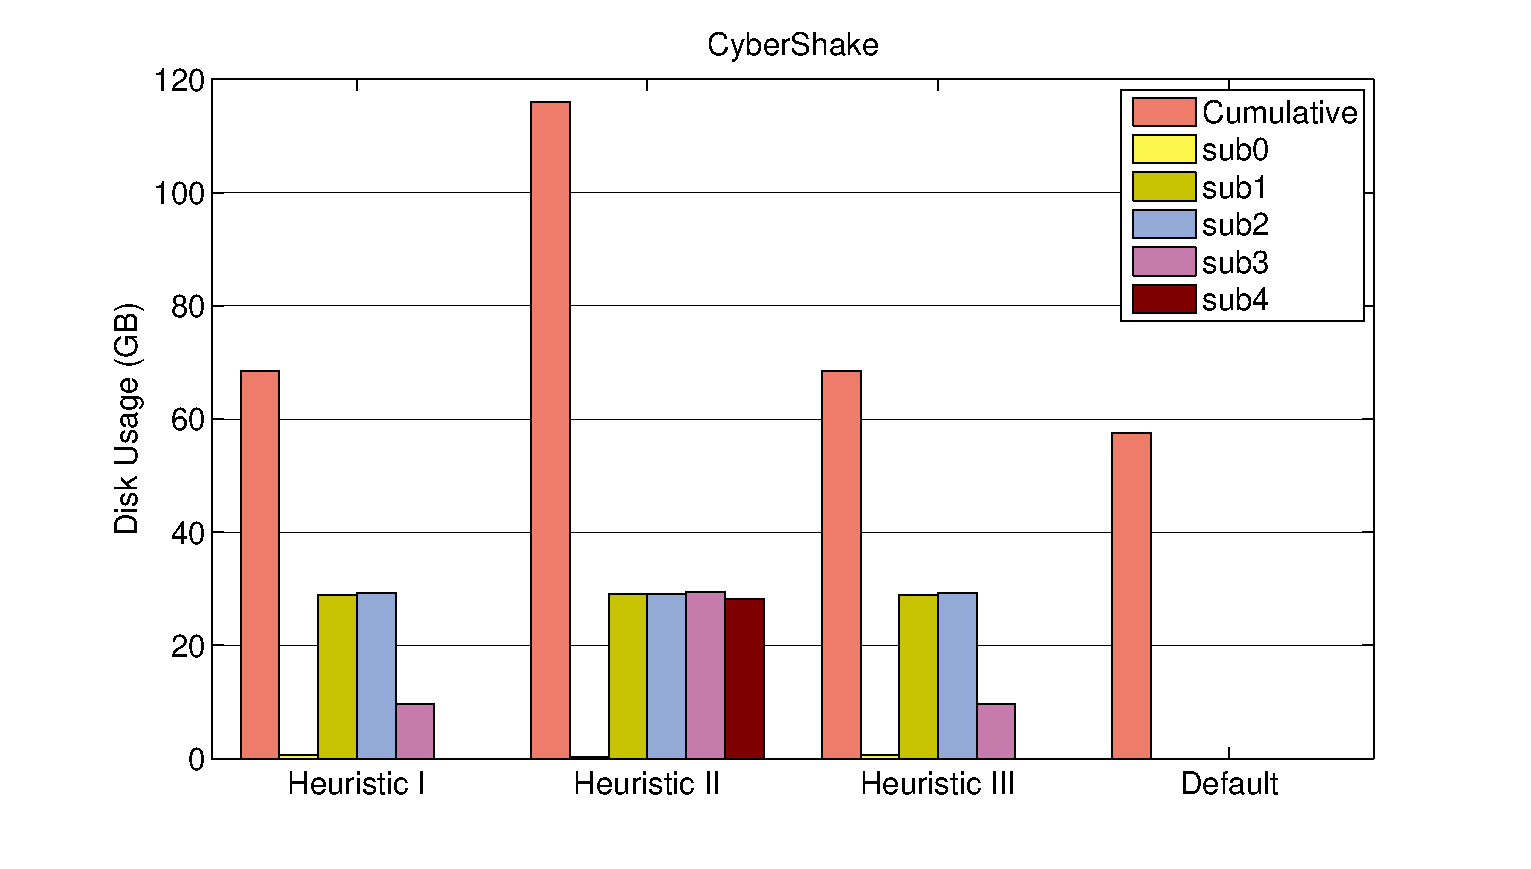
\includegraphics[width=0.8\textwidth]{figures/partitioning/heuristics_usage.eps}
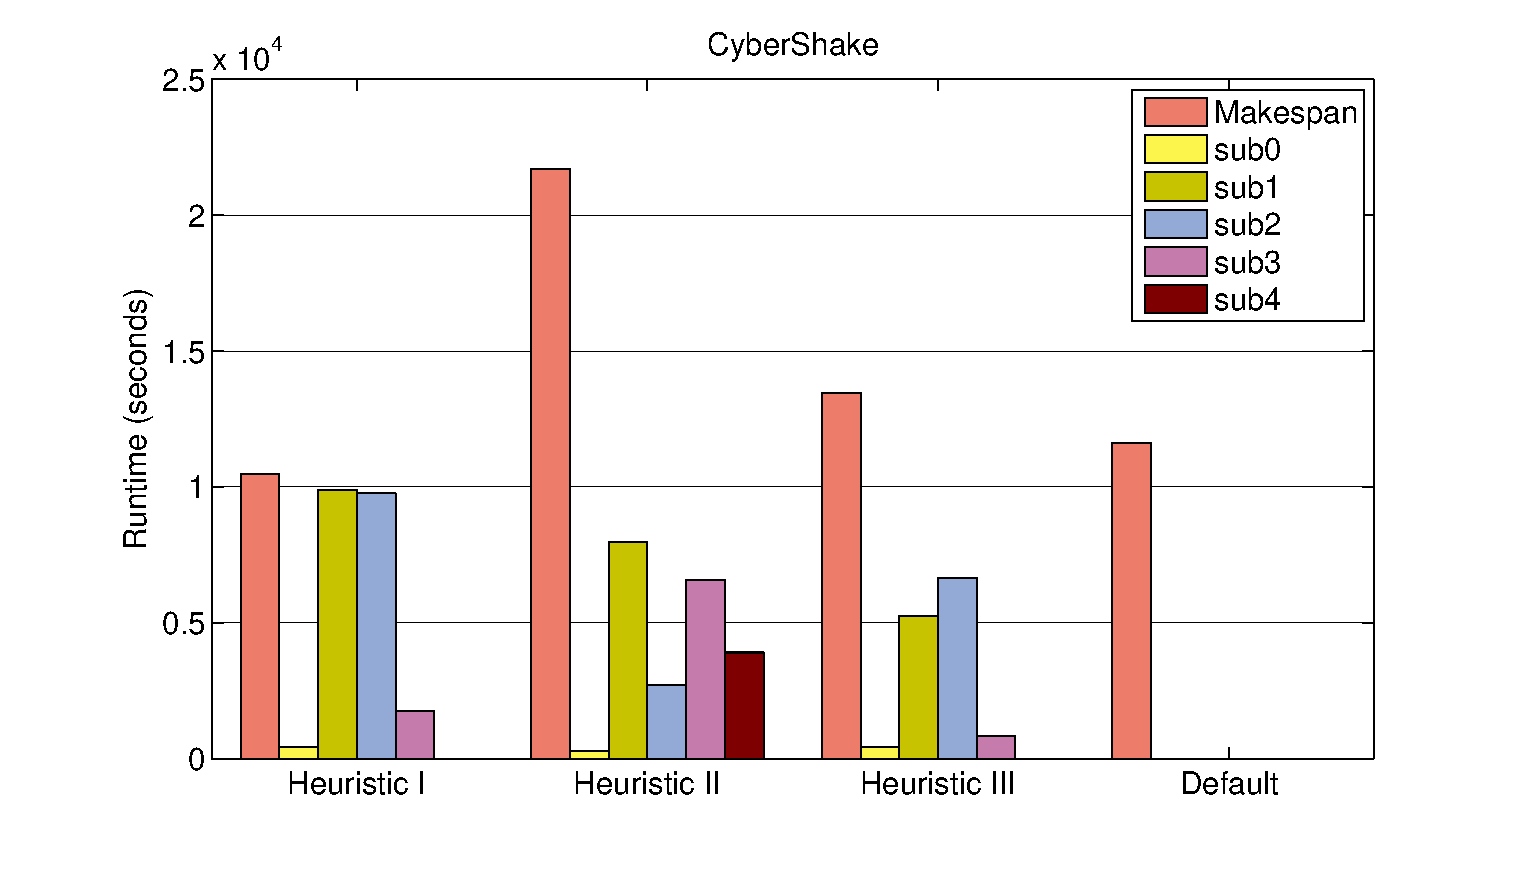
\includegraphics[width=0.8\textwidth]{figures/partitioning/heuristics_makespan.eps}
    \caption{Performance of the three heuristics. The default workflow has one execution site with 4 VMs and 8 Condor slots and has no storage constraint.}
    \label{fig:heuristics}
\end{figure}



%\begin{figure}[h!]
%	\centering
%    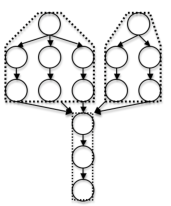
\includegraphics[width=0.3\textwidth]{figures/partitioning/heuristicsI.pdf}
% 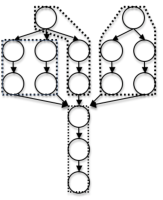
\includegraphics[width=0.3\textwidth]{figures/partitioning/heuristicsII.pdf}
% 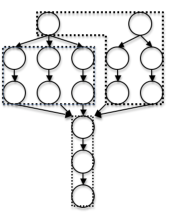
\includegraphics[width=0.3\textwidth]{figures/partitioning/heuristicsIII.pdf}
%    \caption{From left to right: Heuristic I, Heuristic II, Heuristic III.}
%    \label{fig:three_heuristics}
%\end{figure}





\begin{figure}[h!]
	\centering
    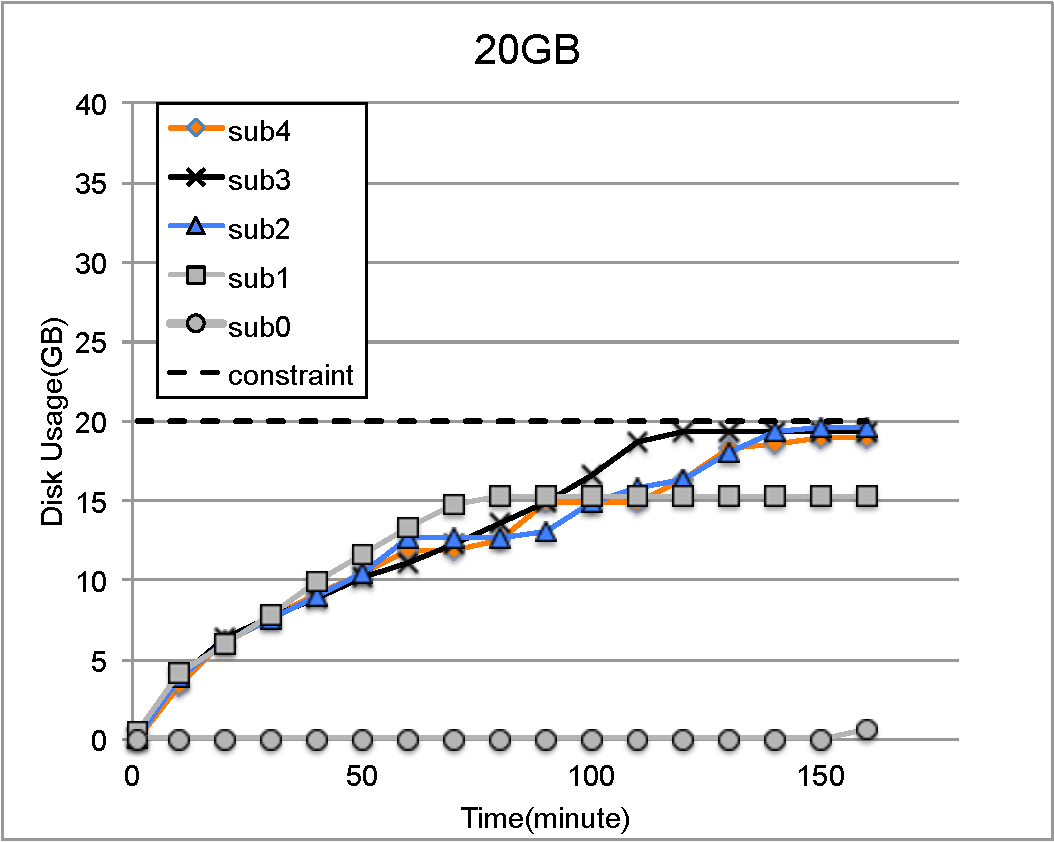
\includegraphics[width=0.49\textwidth]{figures/partitioning/cybershake20gb.pdf}
 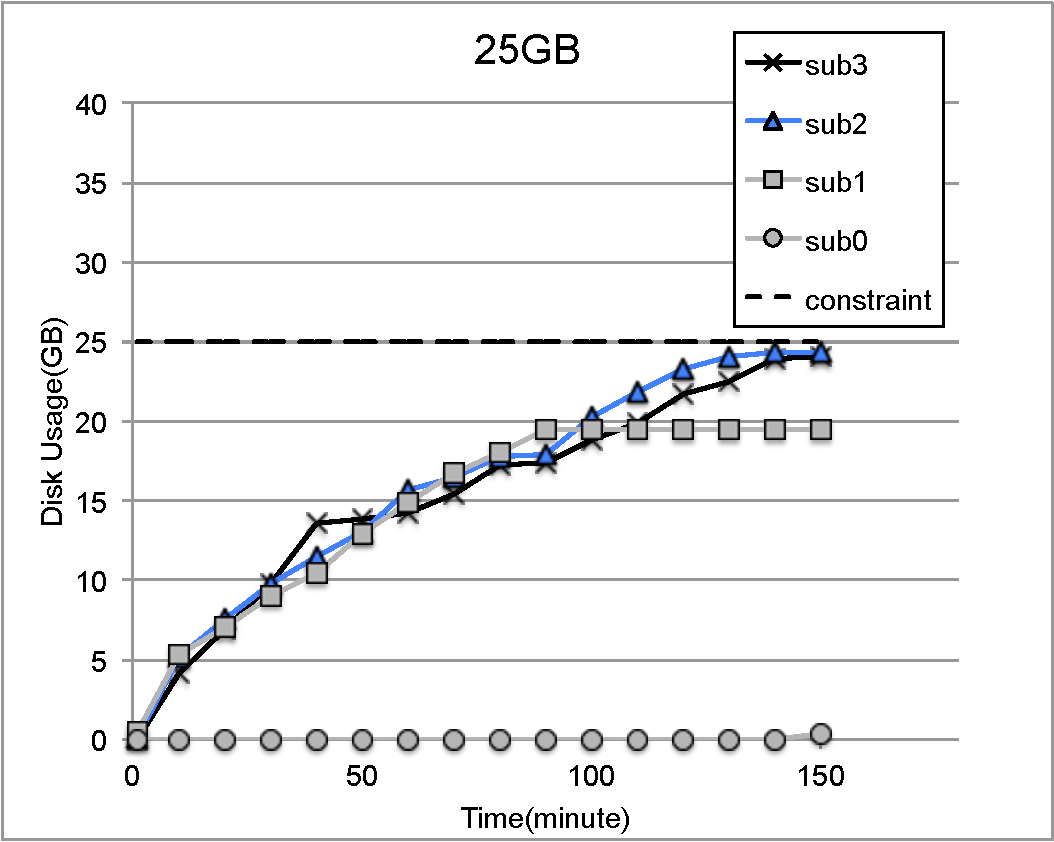
\includegraphics[width=0.49\textwidth]{figures/partitioning/cybershake25gb.pdf}
 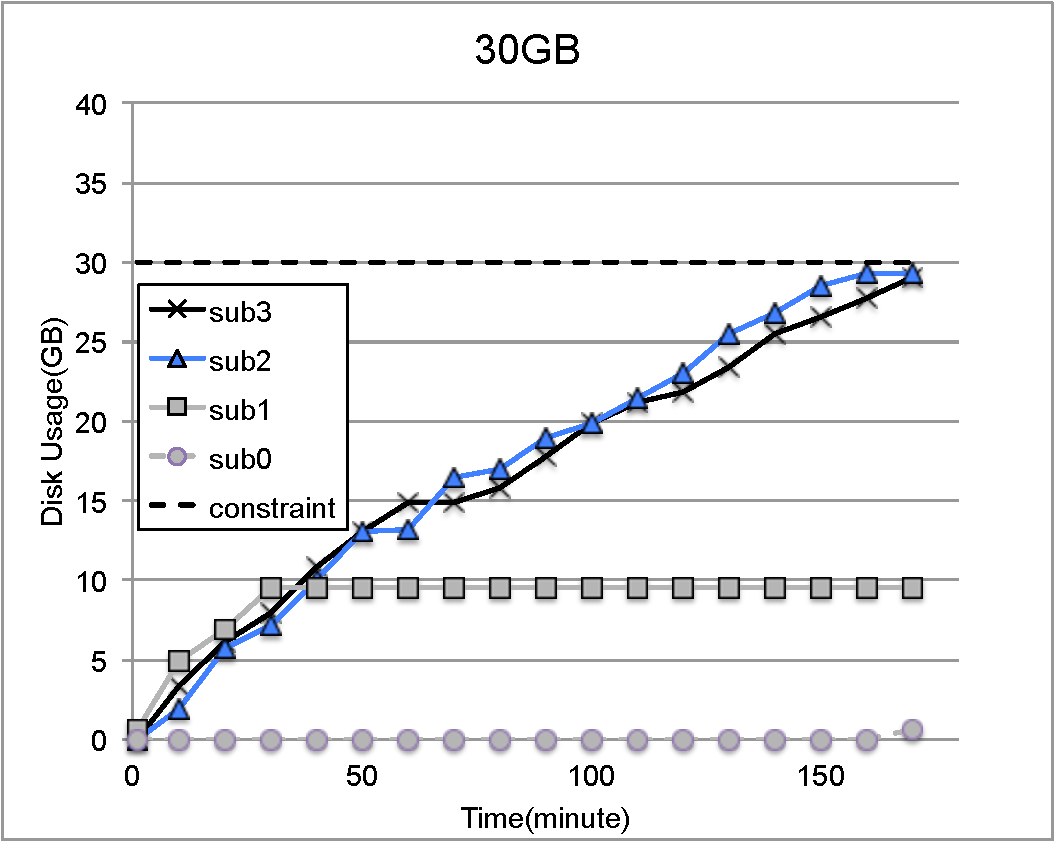
\includegraphics[width=0.49\textwidth]{figures/partitioning/cybershake30gb.pdf}
 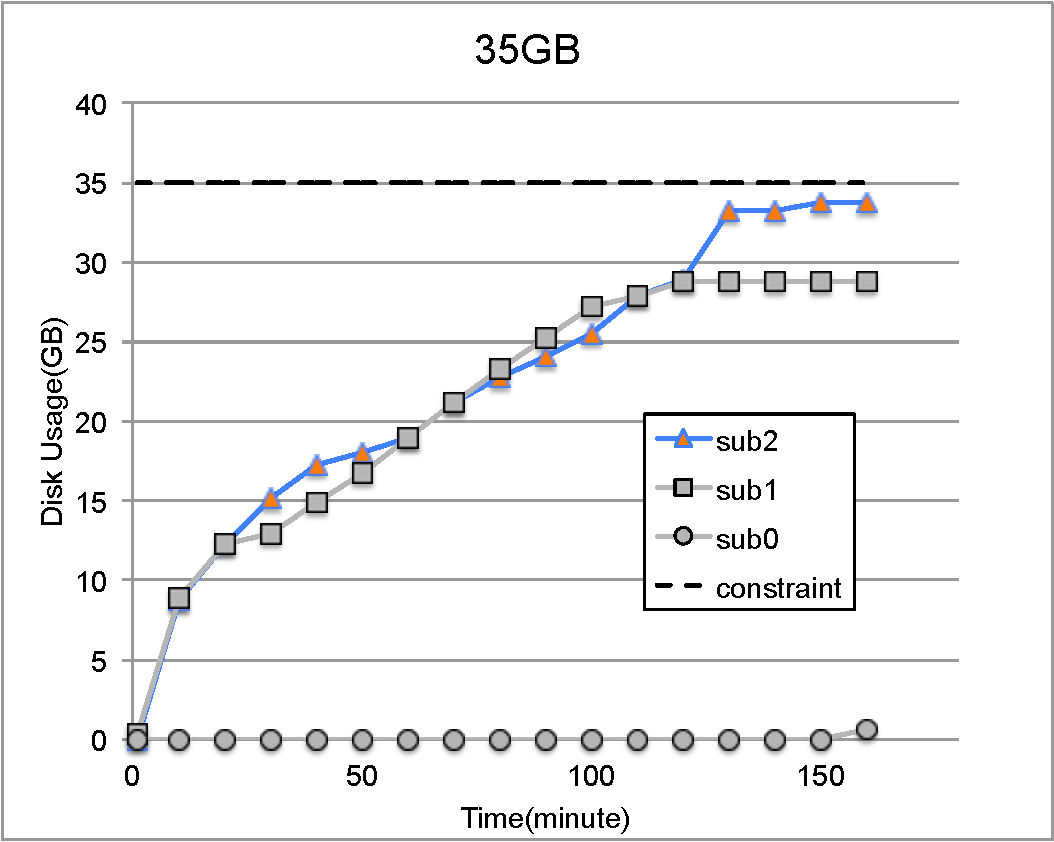
\includegraphics[width=0.49\textwidth]{figures/partitioning/cybershake35gb.pdf}
    \caption{CyberShake with storage constraints of 35GB, 30GB, 25GB, and 20GB. They have 3, 4, 4, and 5 sub-workflows and require 2, 3, 3, and 4 sites to run respectively. }
    \label{fig:constraint}
\end{figure}

\begin{table}[h!]
\caption{CyberShake with Storage Constraint}
\label{tab:constraint}
\centering
\begin{tabular}{lrrrr}
\hline
 storage constraint    &    site &    Disk Usage(GB) &   Percentage  \\
\hline
35GB & A & sub0:0.06; sub1:33.8 & 97\%&\\
& B & sub2:28.8&82\% &\\
30GB & A & sub0:0.07;sub1:29.0 & 97\% \\
& B & sub2:29.3&98\% &\\
& C & sub3:28.8&96\% &\\
25GB & A & sub0:0.06;sub1:24.1 & 97\%& \\

 & B & sub2:24.4 & 98\%& \\
&C&sub3:19.5&78\%&\\
20GB&A&sub0:0.06;sub1:18.9&95\%&\\
&B&sub2:19.3&97\%&\\
&C&sub3:19.6&98\%&\\
&D&sub4:15.3&77\%&\\
\hline
\end{tabular}
\end{table} 


\textbf{Performance Metrics.} To evaluate the performance, we use two types of metrics. Satisfying the Storage Constraints is the main goal of our work in order to fit the sub-workflows into the available storage resources. We compare the results of different storage constraints and heuristics. Improving the Runtime Performance is the second metric that is concerned with in order to minimize the overall makespan. We compare the results of different partitioners, estimators and schedulers. 

\textbf{Workflows Used}. We ran three different workflow applications: an astronomy application (Montage), a seismology application (CyberShake) and a bioinformatics application (Epigenomics). They were chosen because they represent a wide range of application domains and a variety of resource requirements \cite{Juve2009}. 
%For example, Montage is I/O intensive, CyberShake is memory intensive, and Epigenomics is CPU intensive. The goal of the CyberShake Project \cite{Maechling2007} is to calculate Probabilistic Seismic Hazard curves for several geographic sites in the Southern California area. We ran one partition in our experiments that has 24,132 tasks and 58GB of overall data. Montage \cite{Berriman2004} is an astronomy application that is used to construct large image mosaics of the sky. We ran a Montage workflow with a size of 8 degree square of sky. The workflow has 10,422 tasks and 57GB of overall data. Epigenomics \cite{Epigenome} maps short DNA segments collected with high-throughput gene sequencing machines to a reference genome. The workflow has 1,586 tasks and 23GB of overall data. We ran each workflow instance 5 times to account for system variability. 



\begin{figure}[h!]
	\centering
    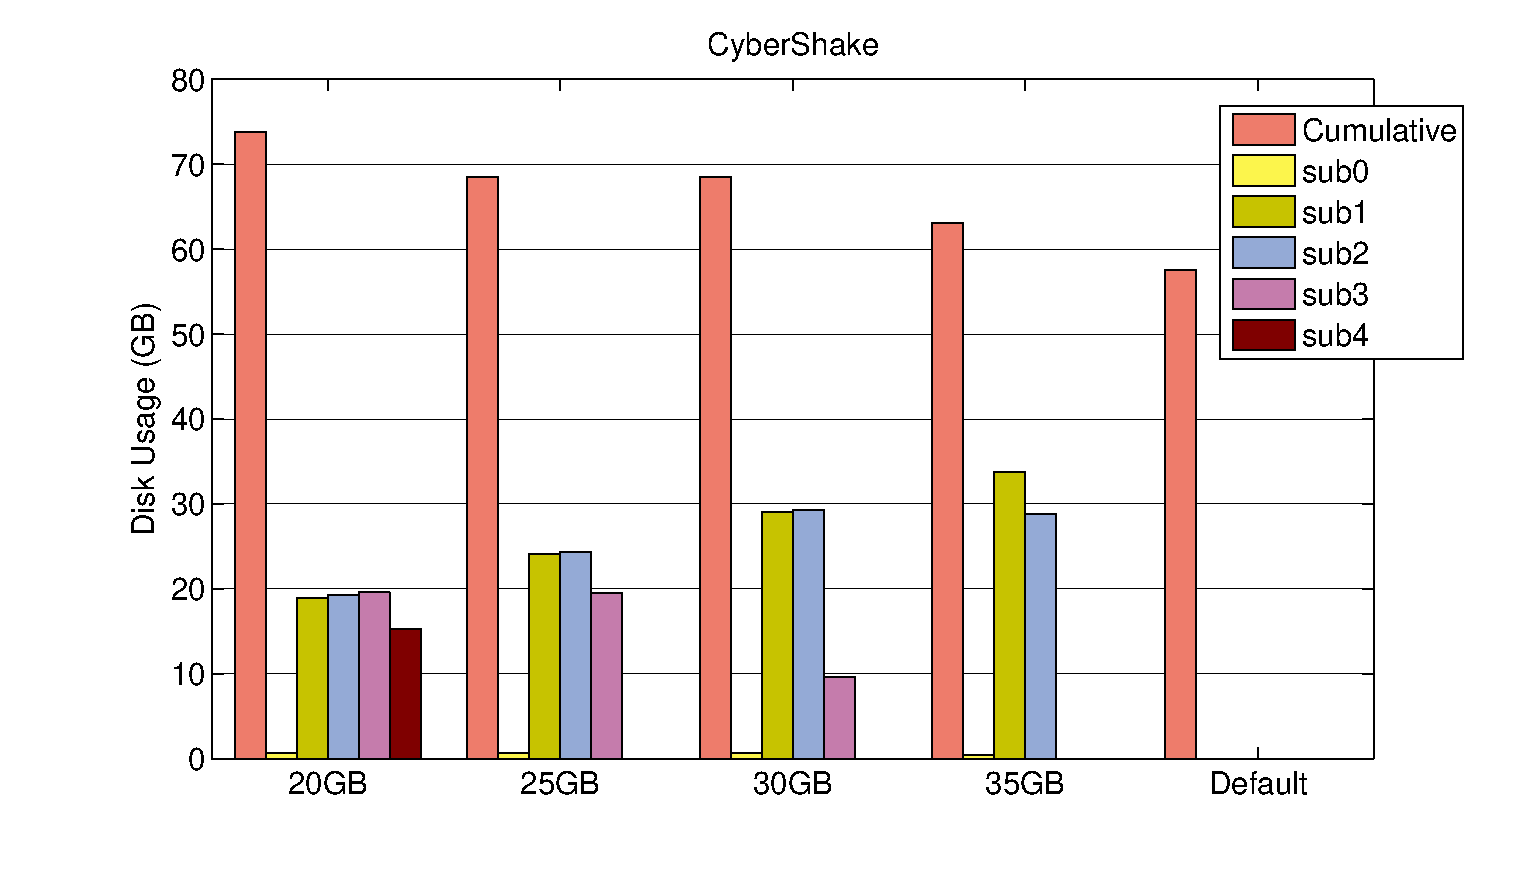
\includegraphics[width=0.8\textwidth]{figures/partitioning/cybershake_usage.eps}
 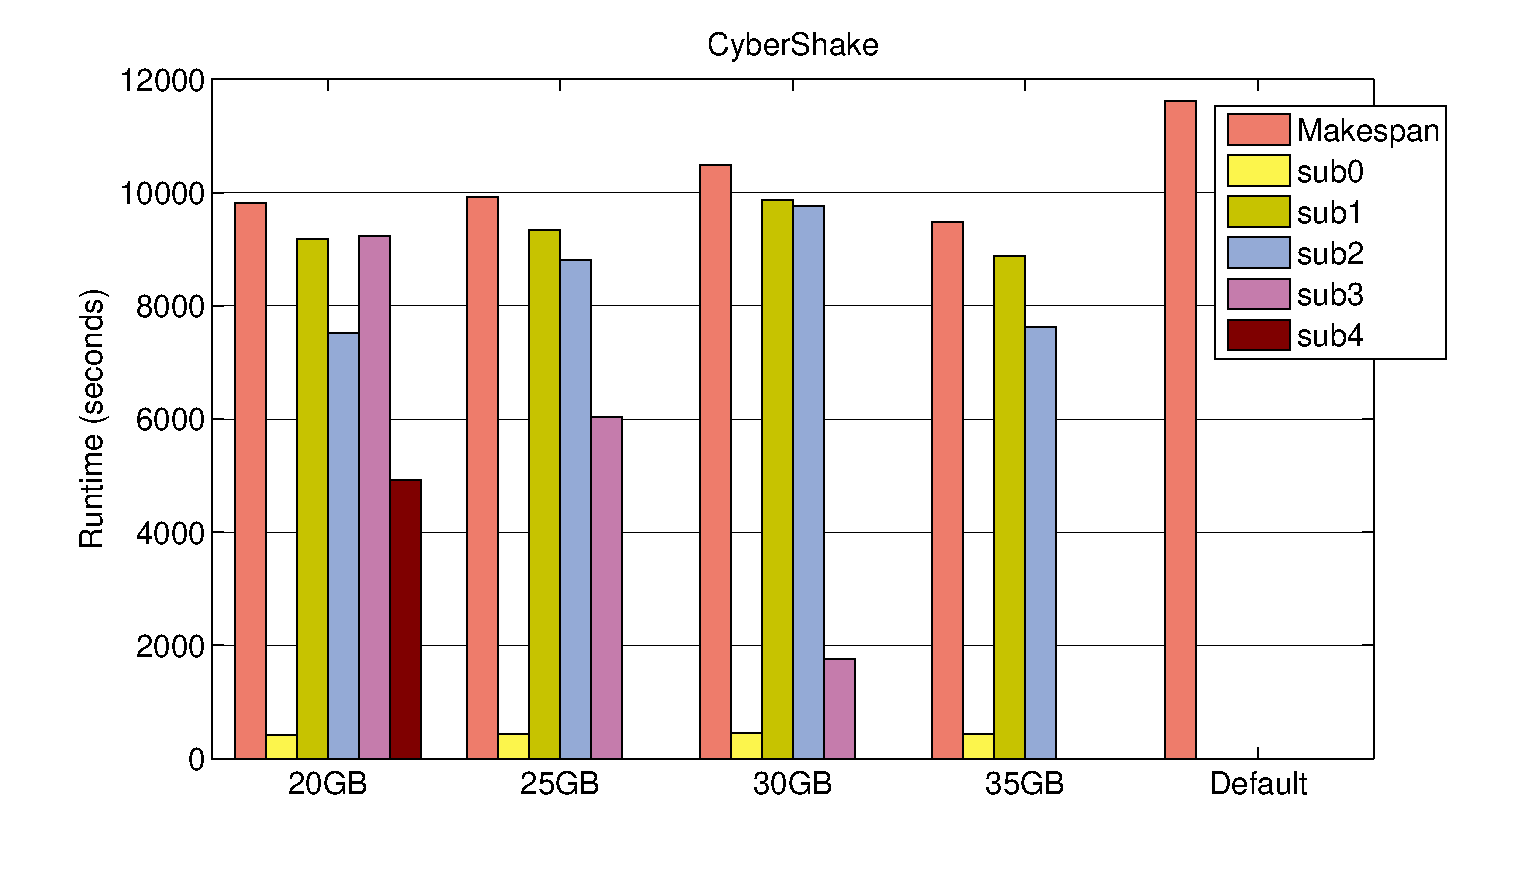
\includegraphics[width=0.8\textwidth]{figures/partitioning/cybershake_makespan.eps}
    \caption{Performance of the CyberShake workflow with different storage constraints}
    \label{fig:cybershake}
\end{figure}



\begin{figure}[h!]
	\centering
    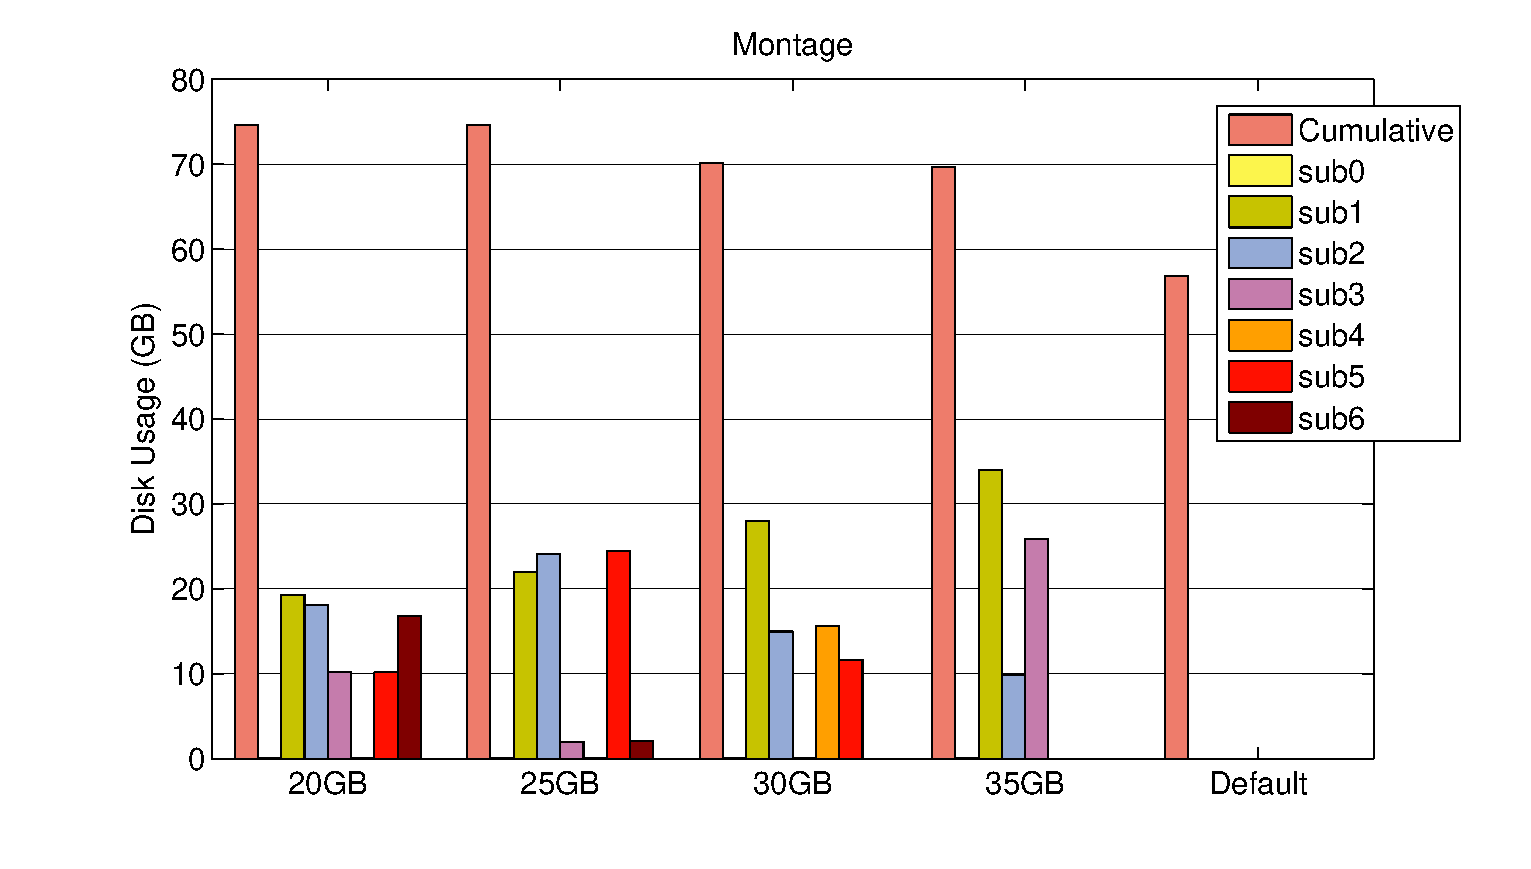
\includegraphics[width=0.8\textwidth]{figures/partitioning/montage_usage.eps}
    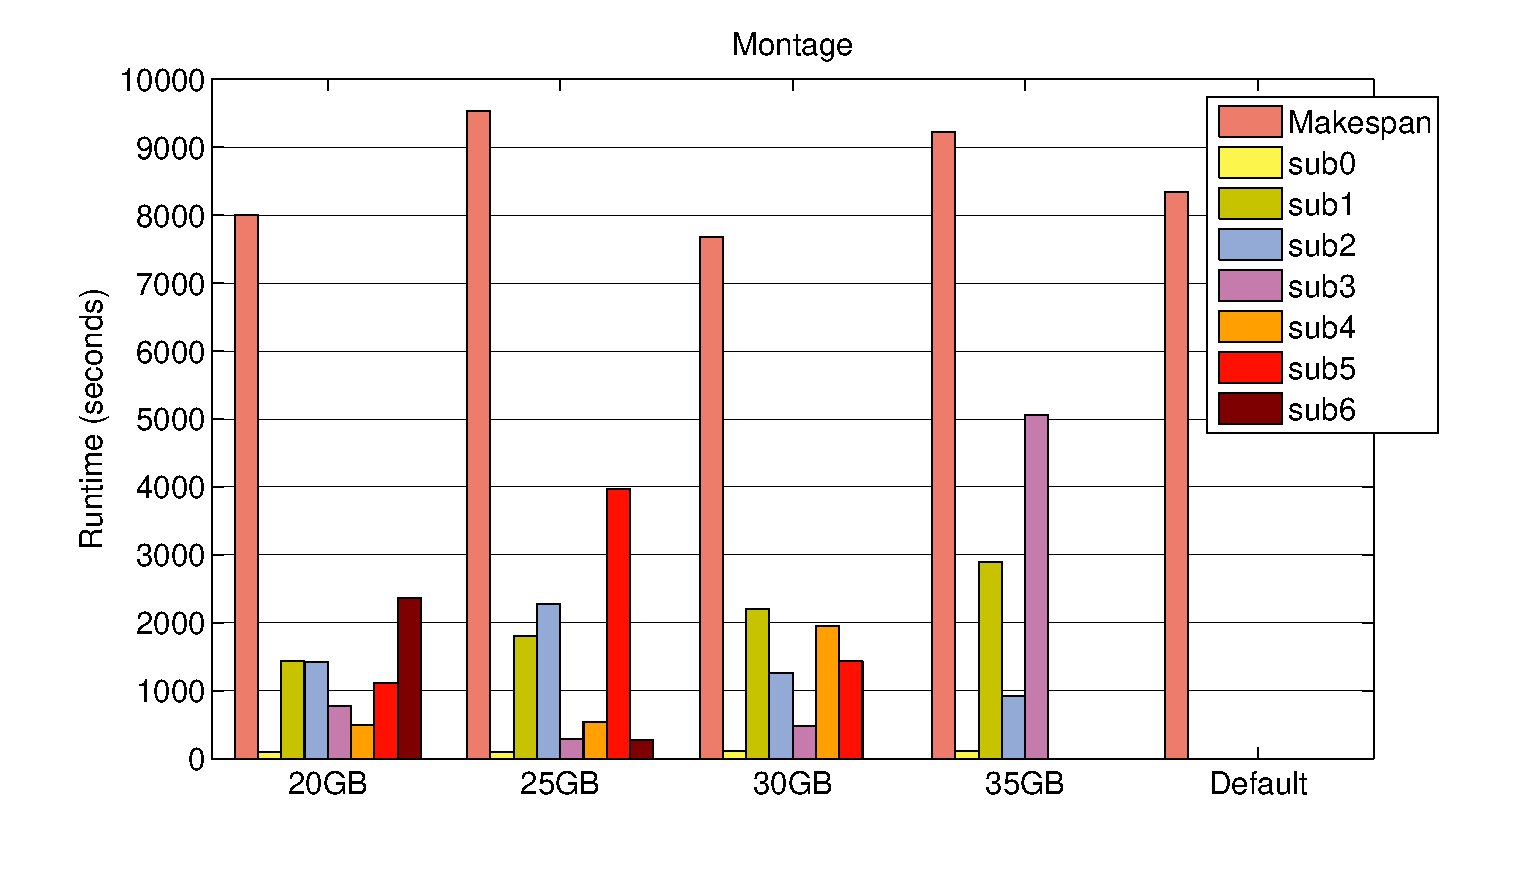
\includegraphics[width=0.8\textwidth]{figures/partitioning/montage_makespan.eps}
    \caption{Performance of the Montage workflow with different storage constraints}
    \label{fig:montage}
\end{figure}

\begin{figure}[h!]
	\centering
    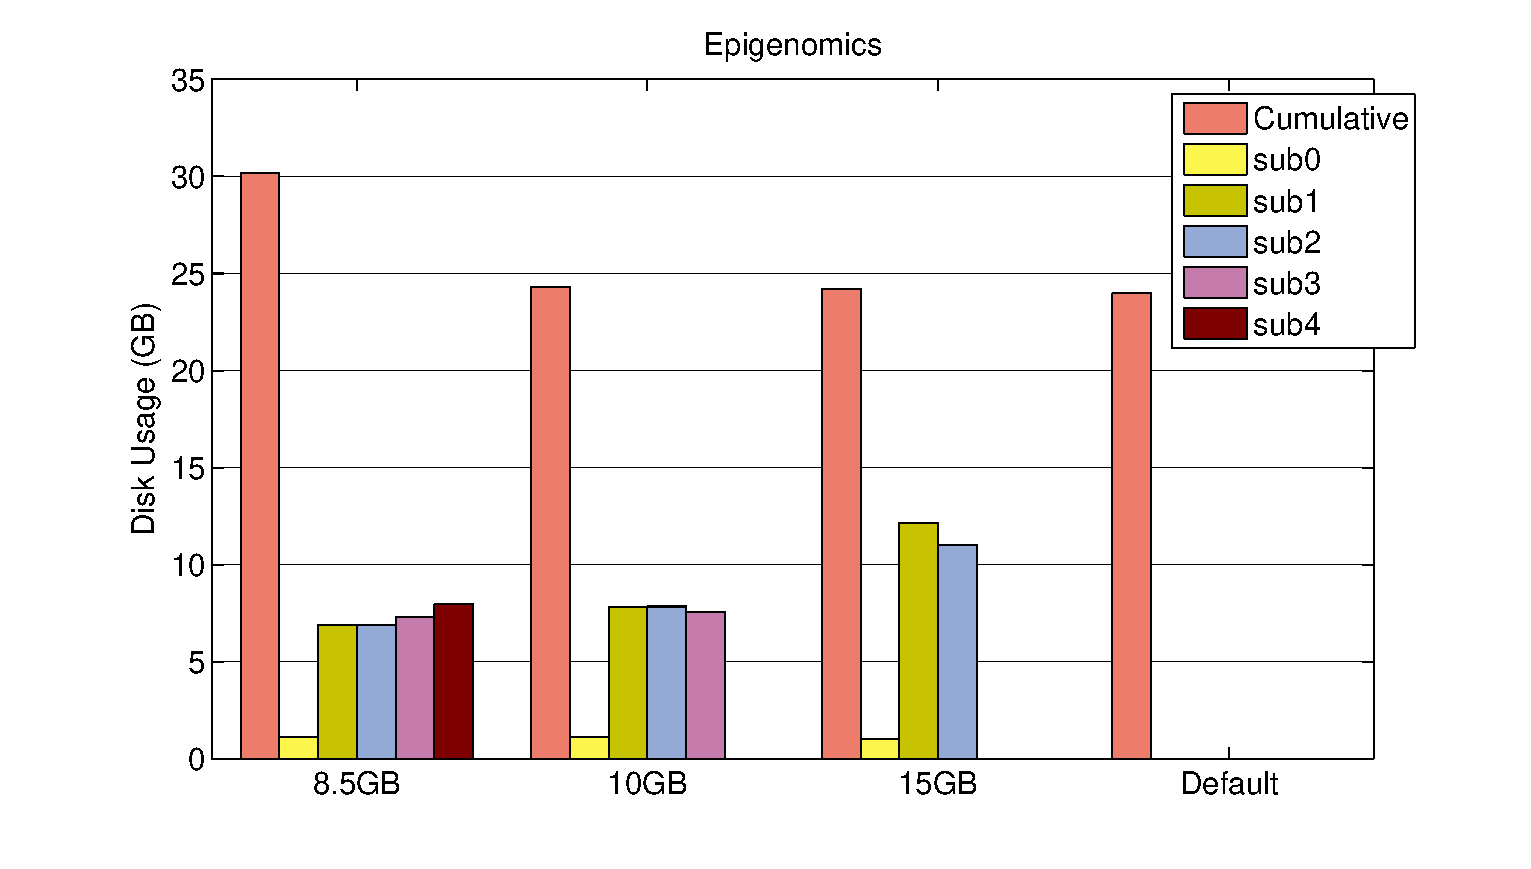
\includegraphics[width=0.8\textwidth]{figures/partitioning/genome_usage.eps}
    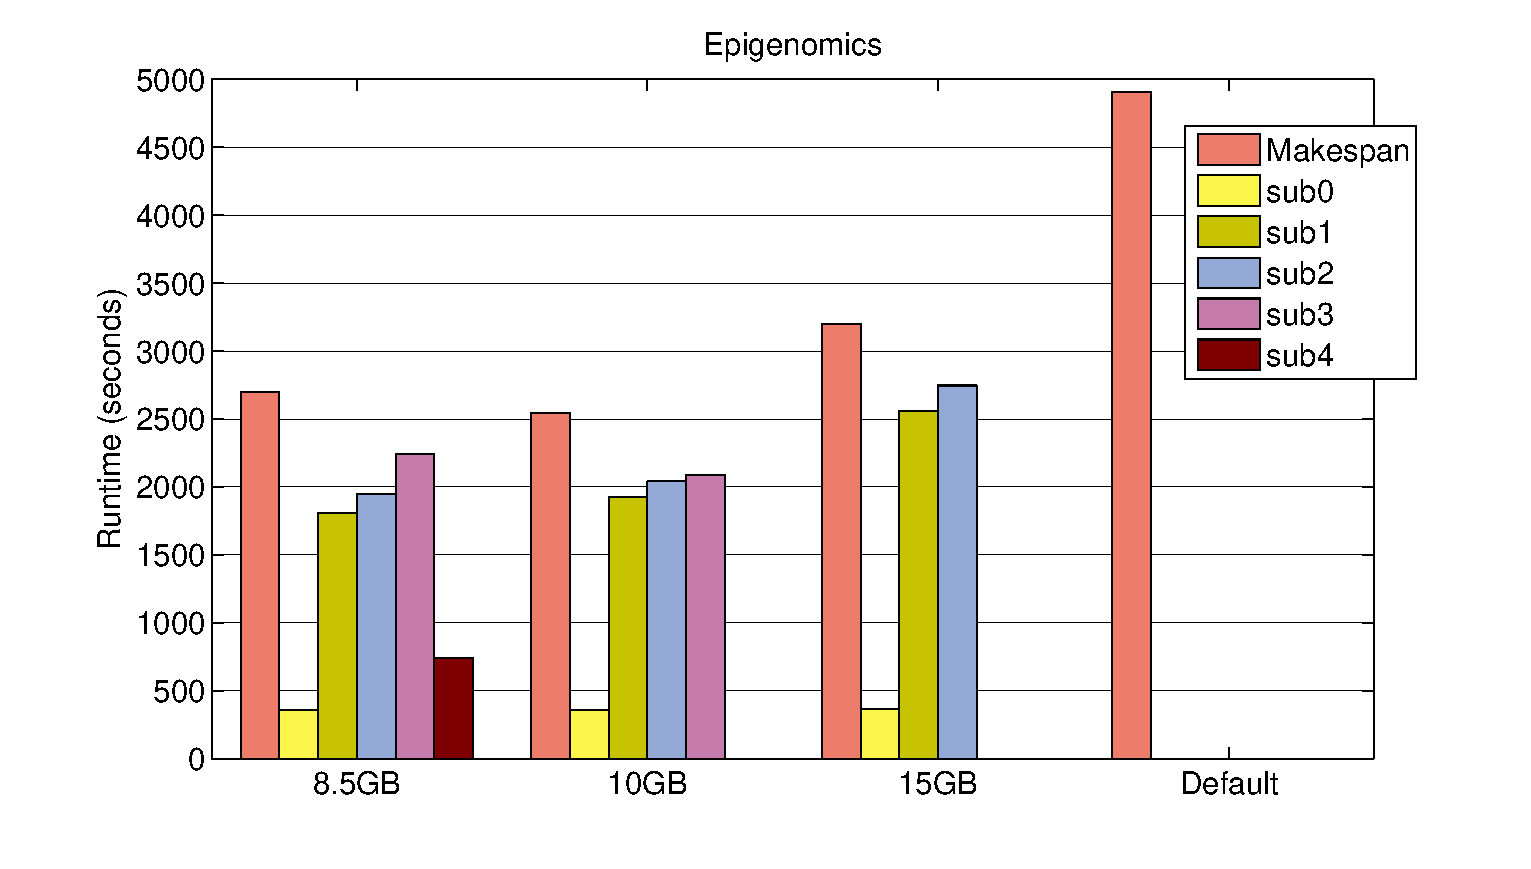
\includegraphics[width=0.8\textwidth]{figures/partitioning/genome_makespan.eps}
    \caption{Performance of the Epigenomics workflow with different storage constraints}
    \label{fig:montage}
\end{figure}

\textbf{Performance of Different Heuristics}. We compare the three heuristics with the CyberShake application. The storage constraint for each site is 30GB. Heuristic II produces 5 sub-workflows with 10 dependencies between them. Heuristic I produces 4 sub-workflows and 3 dependencies. Heuristic III produces 4 sub-workflows and 5 dependencies. The results are shown in Figure~\ref{fig:heuristics} and Heuristic I performs better in terms of both runtime reduction and disk usage. This is due to the way it handles the cross dependency. Heuristic II or Heuristic III simply adds a job if it does not violate the storage constraints or the cross dependency constraints. Furthermore, Heuristic I puts the entire fan structure into the same sub-workflow if possible and therefore reduces the dependencies between sub-workflows. 
%In Figure~\ref{fig:three_heuristics} with an example of a simplified CyberShake workflow, Heuristic I runs two sub-workflows in parallel while the other two have to run them in sequence. 
From now on, we only use Heuristic I in the partitioner in our experiments below.  

\begin{figure}[h!]
	\centering
    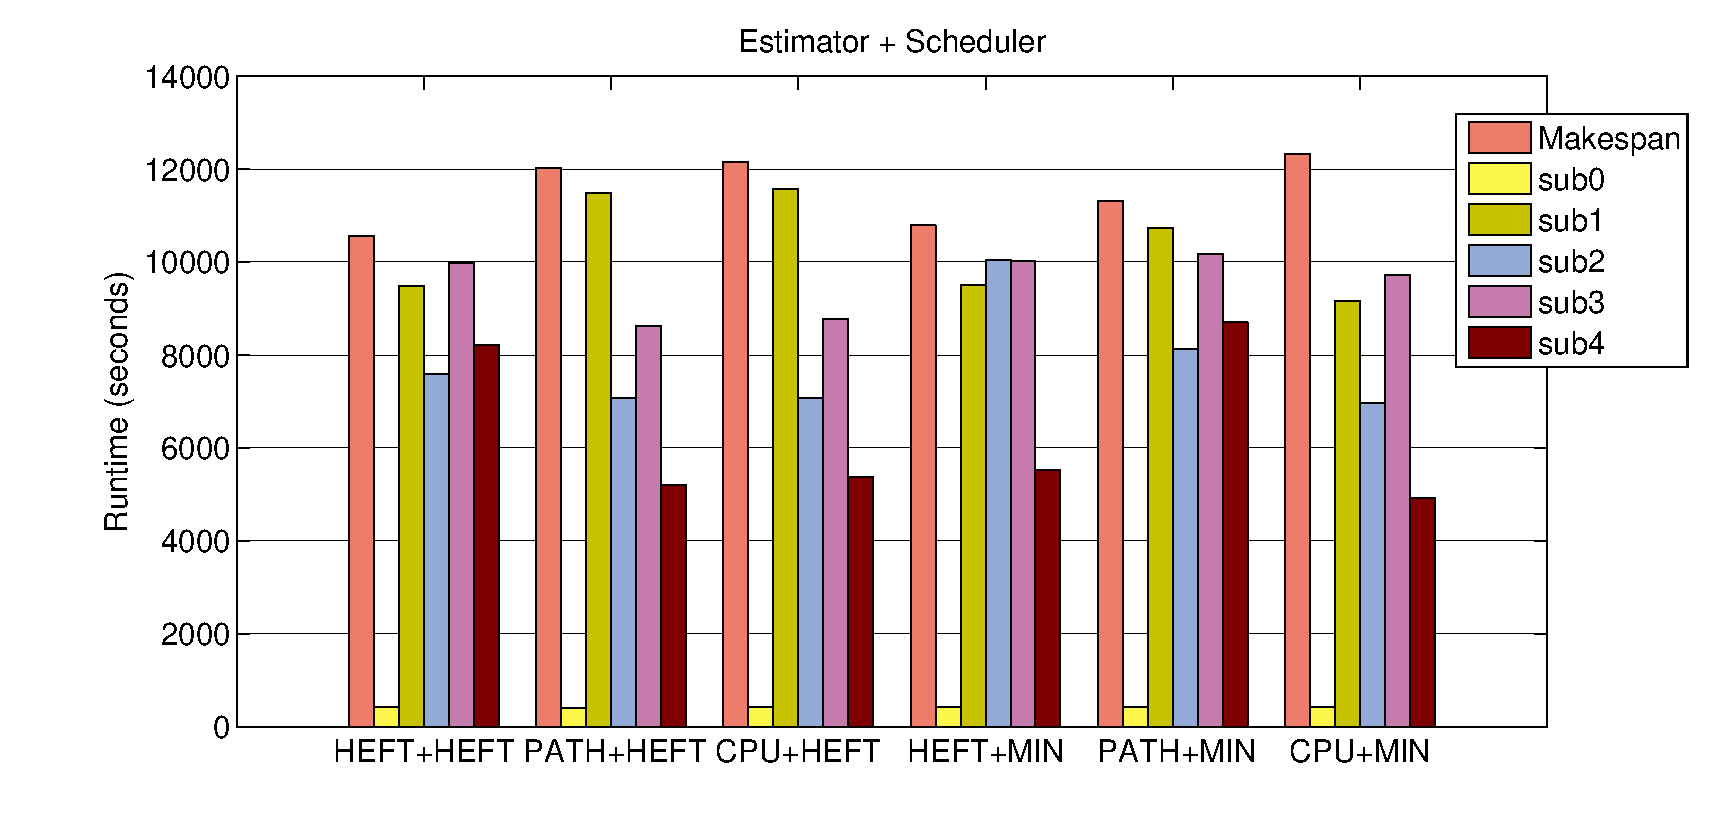
\includegraphics[width=0.9\textwidth]{figures/partitioning/estimator.eps}
    \caption{Performance of estimators and schedulers}
    \label{fig:scheduler}
\end{figure}

\begin{table}[h!]
\caption{Performance of estimators and schedulers}
\label{tab:scheduler}
\centering
\begin{tabular}{lrrrr}
\hline
Combination     &     Estimator &     Scheduler &    Makespan(second)  \\
\hline
HEFT+HEFT & HEFT & HEFT & 10559.5\\
PATH+HEFT & Critical Path & HEFT & 12025.4\\
CPU+HEFT & Average CPU Time & HEFT & 12149.2\\
HEFT+MIN & HEFT & MinMin & 10790 \\
PATH+MIN & Critical Path & MinMin & 11307.2 \\
CPU+MIN & Average CPU Time & MinMin & 12323.2\\
\hline
\end{tabular}
\end{table} 

\textbf{Performance with Different Storage Constraints}. Figure~\ref{fig:constraint} and Table~\ref{tab:constraint} depict the disk usage of the CyberShake workflows over time with storage constraints of 35GB, 30GB, 25GB, and 20GB. They are chosen because they represent a variety of required execution sites. Figure~\ref{fig:cybershake} depicts the performance of both disk usage and runtime. Storage constraints for all of the sub-workflows are satisfied. Among them sub1, sub2, sub3 (if exists), and sub4 (if exists) are run in parallel and then sub0 aggregates their work. The CyberShake workflow across two sites with a storage constraint of 35GB performs best. The makespan (overall completion time) improves by 18.38\% and the cumulative disk usage increases by 9.5\% compared to the default workflow without partitioning or storage constraints. The cumulative data usage is increased because some shared data is transferred to multiple sites. Workflows with more sites to run on do not have a smaller makespan because they require more data transfer even though the computation part is improved. 

Figure~\ref{fig:montage} depicts the performance of Montage with storage constraints ranging from 20GB to 35GB and Epigenomics with storage constraints ranging from 8.5GB to 15GB. The Montage workflow across three sites with 30GB disk space performs best with 8.1\% improvement in makespan and the cumulative disk usage increases by 23.5\%. The Epigenomics workflow across three sites with 10GB storage constraints performs best with 48.1\% reduction in makespan and only 1.4\% increase in cumulative storage. The reason why Montage performs worse is related to its complex internal structures. Montage has two levels of fan-out-fan-in structures and each level has complex dependencies between them.
% as shown in Figure~\ref{fig:workflow}. Our heuristic is not able to untie them thoroughly and therefore the cost of data transfer increases and the sub-workflows are not able to run in parallel.

\textbf{Site selection}. To show the performance of site selection for each sub-workflow, we use three estimators and two schedulers  together with the CyberShake workflow. We build four execution sites with 4, 8, 10 and 10 Condor slots respectively. The labels in Figure~\ref{fig:scheduler} and Table~\ref{tab:scheduler} are defined in a way of ‘Estimator + Scheduler’. For example, HEFT+HEFT denotes a combination of HEFT estimator and HEFT scheduler, which performs best as we expected. The Average CPU Time (or ‘CPU’ in Figure 4.7) does not take the dependencies into consideration and the Critical Path (or ‘PATH’ in Figure~\ref{fig:scheduler}) does not consider the resource availability. The HEFT scheduler is slightly better than MinMin scheduler (or ‘MIN’ in Figure~\ref{fig:scheduler}). Although HEFT scheduler uses a global optimization algorithm compared to MinMin’s local optimization, the complexity of scheduling sub-workflows has been greatly reduced compared to scheduling a vast number of individual tasks. Therefore, both local and global optimization algorithms are able to handle such situations well.

In conclusion, we provide a solution to address the problem of scheduling large workflows across multiple sites with storage constraints. The approach relies on partitioning the workflow into valid sub-workflows. Three heuristics are proposed and compared to show the close relationship between cross dependency and runtime improvement. The performance with three workflows shows that this approach is able to satisfy the storage constraints and reduce the makespan significantly especially for Epigenomics which has fewer fan-in (synchronization) jobs. For the workflows we used, scheduling them onto two or three execution sites is best due to a tradeoff between increased data transfer and increased parallelism. Site selection shows that the global optimization and local optimization perform almost the same.  

\section{Summary}


In this chapter, we propose a framework of partitioning and scheduling large workflows to provide a fine granularity adjustment of workflow activities. We have proposed three heuristics to improve the data aware partitioning and experiments show that our heuristics significantly improve the overall performance including reducing intermediate data transfer, disk usage and the overall makespan. Even though we are using data constraint as an example in this chapter, our approach can be simply modified to apply to other constraints such as CPU, memory and bandwidth. 

After workflow partitioning, we satisfy the resource constraints within an execution site. However, resources within an execution site are not evenly distributed and the balancing between computation and communication is another challenge. In next chapter, we will introduce our balanced task clustering to address this issue. 


\chapter{Balanced Clustering} 
\label{chap:balance}

In this chapter, we examine the reasons that cause load imbalance in task clustering. Furthermore, we propose a series of task balancing methods to address these imbalance problems. A trace-based simulation shows our methods can significantly improve the runtime performance of five widely used workflows compared to the naive implementation of task clustering.

\section{Motivation}


Existing task clustering strategies have demonstrated their effect in some scientific workflows such as CyberShake \cite{Rynge2012} and LIGO \cite{Deelman2002}. However, there are several challenges that are not yet addressed. 

The first challenge users face when executing workflows is task runtime variation. 
%Tasks may have diverse task runtimes and such diversity may cause some load imbalance. The last completed task among a given set of tasks essentially controls the release of next set of tasks. 
In a scientific workflow, tasks within a level (or depth within a workflow directed acyclic graph) may have different runtimes. Merging tasks within a level without considering the runtime variance may cause load imbalance, i.e., some clustered jobs may be composed of short running tasks while others of long running tasks. This imbalance delays the release of tasks from the next level of the workflow, penalizing the workflow execution with an overhead produced by the use of inappropriate task clustering strategies.
A common technique to handle load imbalance is overdecomposition~\cite{Lifflander2012}.
This method decomposes computational work into medium-grained balanced tasks. Each task is coarse-grained enough to enable efficient execution and reduce scheduling overheads, while being fine-grained enough to expose significantly higher application-level parallelism than what is offered by the hardware. 

The second challenge has to do with the complex data dependencies within a workflow. 
Merging tasks that have no intermediate data between them seems safe at the first sight. However, the subsequent tasks that rely on the output data that their parent tasks produce may suffer a data locality problem since data may be distributed poorly and the data transfer time is increased.  As a result, data transfer times and failure probabilities increase. Therefore, we claim that data dependencies of subsequent tasks should be considered.


%We generalize these two challenges (Runtime Imbalance and Dependency Imbalance) to the general imbalance problem. It means that the execution of workflows suffers from significant overheads (unavailable data, overloaded resources, or system constraints) due to inappropriate task clustering and job execution. To solve the imbalance problem, we introduce a series of balancing methods to address these two challenges respectively. 
%This is from FGCS
We generalize these two challenges (Runtime Imbalance and Dependency Imbalance) to the general load balance problem. We introduce a series of balancing methods to address these challenges. However, there is a tradeoff between runtime and data dependency balancing. For instance, balancing runtime may aggravate the Dependency Imbalance problem, and vice versa. Therefore, we propose a series of quantitative metrics that reflect the internal structure (in terms of task runtimes and dependencies) of the workflow and use them as a criterion to select and balance these solutions.

%However, what makes this problem challenging is that the solutions are usually conflicting. For example, balancing runtime may worsen the Dependency Imbalance problem, and vice versa. A quantitative measurement of workflow characteristics is required to serve as a criterion to select and balance these solutions. To achieve this goal, we propose four metrics to reflect the internal structure (in terms of runtime and dependency) of the workflow. 

In particular, we provide a novel approach to capture these metrics. Traditionally, there are two approaches to improve the performance of task clustering. The first one is a top-down approach \cite{Integration2012} that represents the clustering problem as a global optimization problem and aims to minimize the overall runtime of a workflow. However, the complexity of solving such an optimization problem does not scale well. The second one is a bottom-up approach \cite{Muthuvelu2005}\cite{Liu2009} that only examines free tasks to be merged and optimizes the clustering results locally. In contrast, our work extends these solutions to consider the neighboring tasks including siblings, parents, children and so on because such a family of tasks has strong connections between them. 

%The third contribution we make is that we analyze and connect the performance of these metrics and balancing methods. These quantitative metrics indicate which type of imbalance problem a workflow is more likely to suffer from. Comparing the relative values of these metrics informs the selection of a balancing method or a combination of these methods. 
In this chapter, we address the balancing problem by studying (\emph{i}) the performance gain of using our balancing methods over a baseline execution on a larger set of workflows; (\emph{ii}) the performance gain over two additional task clustering methods in literature; (\emph{iii}) the performance impact of the variation of the average data size and the number of resources; and (\emph{iv}) the performance impact of combining our balancing methods with vertical clustering.




\section{Approach}


 In this section, we introduce metrics that quantitatively capture workflow characteristics to measure runtime and dependence imbalances. We then present methods to address the load balance problem.



\subsection{Imbalance metrics}

\textbf{Runtime Imbalance} describes the difference of the task/job runtime of a group of tasks/jobs. In this work, we denote the \textbf{Horizontal Runtime Variance} ($HRV$) as the ratio of the standard deviation in task runtime to the average runtime of tasks/jobs at the same horizontal level of a workflow. At the same horizontal level, the job with the longest runtime often controls the release of the next level jobs. A high $HRV$ value means that the release of next level jobs has been delayed. Therefore, to improve runtime performance, it makes sense to reduce the standard deviation of job runtime. Figure~\ref{fig:imbalance_rv} shows an example of four independent tasks $t_1$, $t_2$, $t_3$ and $t_4$ where the task runtime of $t_1$ and $t_2$ is 10 seconds, and the task runtime of $t_3$ and $t_4$ is 30 seconds. In the Horizontal Clustering (HC) approach, a possible clustering result could be merging $t_1$ and $t_2$ into a clustered job, and $t_3$ and $t_4$ into another. This approach results in imbalanced runtime, i.e., $HRV > 0$ (Figure~\ref{fig:imbalance_rv}-top). In contrast, a balanced clustering strategy should try its best to evenly distribute task runtime among jobs as shown in Figure~\ref{fig:imbalance_rv} (bottom). A smaller \emph{HRV} means that the runtime of tasks within a horizontal level is more evenly distributed and therefore it is less necessary to use runtime-based balancing algorithms. However, runtime variance is not able to describe how symmetric the structure of the dependencies between tasks is.

\begin{figure}[htb]
	\centering
	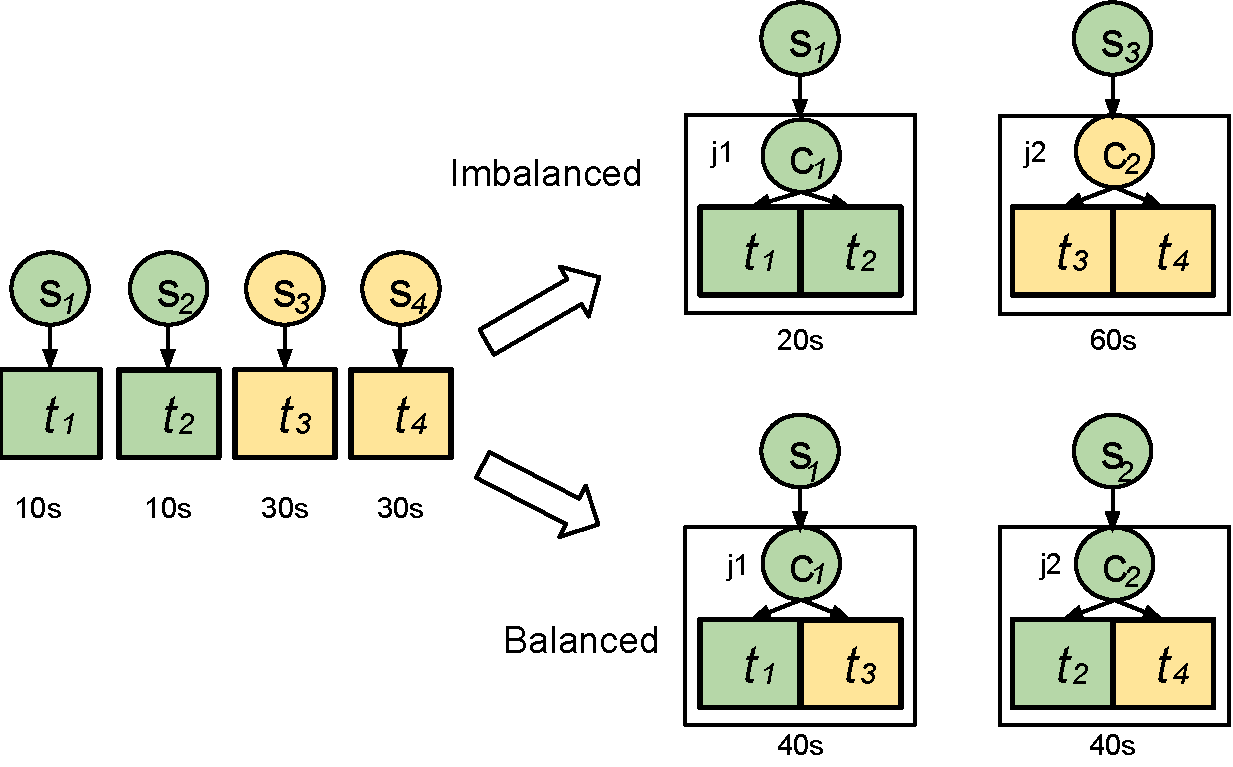
\includegraphics[width=0.8\linewidth]{figures/balance/figure5.pdf}
	\captionof{figure}{An example of Horizontal Runtime Variance.}
	\label{fig:imbalance_rv}
\end{figure}


\textbf{Dependency Imbalance} means that the task clustering at one horizontal level forces the tasks at the next level (or even subsequent levels) to have severe data locality problems and thus loss of parallelism. For example, in Figure~\ref{fig:imbalance_dv}, we show a two-level workflow composed of four tasks in the first level and two in the second. Merging $t_1$ with $t_3$ and $t_2$ with $t_4$ (imbalanced workflow in Figure~\ref{fig:imbalance_dv}) forces $t_5$ and $t_6$ to transfer files from two locations and wait for the completion of $t_1$, $t_2$, $t_3$, and $t_4$.  A balanced clustering strategy groups tasks that have the maximum number of child tasks in common. Thus, $t_5$ can start to execute as soon as $t_1$ and $t_2$ are completed, and so can $t_6$. To measure and quantitatively demonstrate the Dependency Imbalance of a workflow, we propose two  metrics: ($i$) Impact Factor Variance, and ($ii$) Distance Variance. 

\begin{figure}[htb]
	\centering
	\includegraphics[width=0.8\linewidth]{figures/balance/figure6.pdf}
	\captionof{figure}{An example of Dependency Imbalance.}
	\label{fig:imbalance_dv}
\end{figure}

We define the \textbf{Impact Factor Variance} ($IFV$) of tasks as the standard deviation of their impact factors. The \textbf{Impact Factor} ($IF$) of a task $t_u$ is defined as follows:

\begin{equation}
\label{eq:imbalance_impact_factor}
	IF(t_u)=\sum_{t_v\in Child(t_u)}^{}\frac{IF(t_v)}{||Parent(t_v)||}
\end{equation}
where $Child(t_u)$ denotes the set of child tasks of $t_u$, and $||Parent(t_v)||$ the number of parent tasks of $t_v$. The Impact Factor aims at capturing the similarity of tasks/jobs in a graph by measuring their relative impact factor or importance to the entire graph. Tasks with similar impact factors are merged together, so that the workflow structure tends to be more `even' or symmetric. For simplicity, we assume the $IF$ of a workflow exit task (e.g. $t_5$ in Figure~\ref{fig:imbalance_dv}) is 1.0. For instance, consider the two workflows presented in Figure~\ref{fig:imbalance_hifv}. The $IF$ for each of $t_1$, $t_2$, $t_3$, and $t_4$ is computed as follows:

\begin{eqnarray*}
	\displaystyle  
	&IF(t_7 )=1.0, IF(t_6 )=IF(t_5 )=IF(t_7 )/2=0.5\nonumber  \\
	&IF(t_1 )=IF(t_2 )=IF(t_5 )/2=0.25\nonumber \\
	&IF(t_3 )=IF(t_4 )=IF(t_6 )/2=0.25\nonumber 
\end{eqnarray*}

Thus, IFV($t_1$, $t_2$, $t_3$, $t_4$) = 0. In contrast, the $IF$ for $t_{1'}$, $t_{2'}$, $t_{3'}$, and $t_{4'}$ is:

\begin{eqnarray*}
	\displaystyle  
	&IF(t_{7'})=1.0, IF(t_{6'})=IF(t_{5'})=IF(t_{1'})=IF(t_{7'})/2=0.5\nonumber \\
	&IF(t_{2'})=IF(t_{3'})=IF(t_{4'})=IF(t_{6'})/3=0.17 \nonumber
\end{eqnarray*}

Therefore, the $IFV$ value for {$t_{1'}$, $t_{2'}$, $t_{3'}$, $t_{4'}$} is 0.17, which predicts it is likely to be less symmetric than the workflow in Figure~\ref{fig:imbalance_hifv} (left). In this chapter, we use \textbf{HIFV} (Horizontal IFV) to indicate the $IFV$ of tasks at the same horizontal level. The time complexity of calculating the $IF$ of all the tasks of a workflow with $n$ tasks is $O(n)$.  

\begin{figure}[htb]
	\centering
	\includegraphics[width=0.75\linewidth]{figures/balance/figure7.pdf}
	\captionof{figure}{Example of workflows with different data dependencies}
	\label{fig:imbalance_hifv}
\end{figure}

\textbf{Distance Variance} ($DV$) describes how `close' tasks are to each other. The distance between two tasks/jobs is defined as the cumulative length of the path to their closest common successor. If they do not have a common successor, the distance is set to infinity. For a group of $n$ tasks/jobs, the distance between them is represented by a $n \times n$ matrix $D$, where an element $D(u,v)$ denotes the distance between a pair of tasks/jobs $u$ and $v$. For any workflow structure, $D(u,v)=D(v,u)$ and $D(u,u)=0$, thus we ignore the cases when $u \geq v$. Distance Variance is then defined as the standard deviation of all the elements $D(u,v)$ for $u<v$. The time complexity of calculating all the values of $D$ of a workflow with $n$ tasks is $O(n^2)$. 

Similarly, $HDV$ indicates the $DV$ of a group of tasks/jobs at the same horizontal level. For example, Table~\ref{tab:imblance_metric} shows the distance matrices of tasks from the first level for both workflows of Figure~\ref{fig:imbalance_hifv} ($D_1$ for the workflow in the left, and $D_2$ for the workflow in the right). $HDV$ for $t_1, t_2, t_3$, and $t_4$ is 1.03, and for $t_{1'}, t_{2'}, t_{3'}$, and $t_{4'}$ is 1.10. In terms of distance variance, $D_1$ is more `even' than $D_2$. A smaller $HDV$ means that the tasks at the same horizontal level are more equally `distant' from each other and thus the workflow structure tends to be more `even' and symmetric. 

\begin{table}[htb]
	\footnotesize
	\centering
	\begin{tabular}{l|rrrr}
		$D_1$ & $t_1$ & $t_2$ & $t_3$ &$t_4$\\
		\hline
		$t_1$ & 0 & 2 & 4 & 4 \\
		$t_2$ & 2 & 0 & 4 & 4 \\
		$t_3$ & 4 & 4 & 0 & 2\\
		$t_4$ & 4 & 4 & 2 & 0 \\
	\end{tabular}
	\quad
	\begin{tabular}{l|rrrr}
		$D_2$ & $t_1'$ & $t_2'$ & $t_3'$ &$t_4'$\\
		\hline
		$t_1'$ & 0 & 4 & 4 & 4 \\
		$t_2'$ & 4 & 0 & 2 & 2 \\
		$t_3'$ & 4 & 2 & 0 & 2\\
		$t_4'$ & 4 & 2 & 2 & 0 \\
	\end{tabular}
	\caption{Distance matrices of tasks from the first level of workflows in Figure~\ref{fig:imbalance_hifv}.}
	\label{tab:imblance_metric}
\end{table}

In conclusion, runtime variance and dependency variance offer a quantitative and comparable tool to measure and evaluate the internal structure of a workflow. 



\subsection{Balanced clustering methods}
\label{sec:balance:methods}
In this subsection, we introduce our balanced clustering methods used to improve the runtime and dependency balance in task clustering. We first introduce the basic runtime-based clustering method, and then two other balancing methods that address the dependency imbalance problem. 

\begin{algorithm}[!htb]
	\footnotesize
	\caption{Horizontal Runtime Balancing algorithm.}
	\label{alg:imbalance_hrb}
	\begin{algorithmic}[1]
		\Require $W$: workflow; $C$: number of tasks per jobs; $R$: number of jobs per horizontal level
		\Procedure{Clustering}{$W,C$}
			\For{$level < depth(W)$}
				\State $TL\gets $\ \Call{GetTasksAtLevel}{$W,level$} \Comment{Partition $W$ based on depth}
				\State $CL\gets$  \ \Call{Merge}{$TL,C, R$} \Comment{Returns a list of clustered jobs}
				\State $W \gets W - TL + CL$  \Comment{Merge dependencies as well} 
			\EndFor
		\EndProcedure
		\Procedure{Merge}{$TL, C, R$}
			\For{$i<R$}
			\State $J_i\gets$\{\}\Comment{An empty job}
			\EndFor
			\State $CL\gets$\{\}\Comment{An empty list of clustered jobs}
			\State Sort $TL$ in descending of runtime
			\ForAll{$t$ in $TL$}
				\State $J\gets$ the job with shortest runtime and less than $C$ tasks  
				\State $J$.add ($t$) \Comment{Adds the task to the shortest job}
				
			\EndFor
			\For{$i<R$}
			\State  $CL$.add( $J_i$)
			\EndFor
			\State \textbf{return} $CL$
		\EndProcedure
	\end{algorithmic}
\end{algorithm}



\textbf{Horizontal Runtime Balancing} (HRB) aims to evenly distribute task runtime among clustered jobs. Tasks with the longest runtime are added to the job with the shortest runtime. Algorithm~\ref{alg:imbalance_hrb} shows the pseudocode of HRB. This greedy method is used to address the load balance problem caused by runtime variance at the same horizontal level. Figure~\ref{fig:imbalance_hrb} shows an example of HRB where tasks in the first level have different runtimes and should be grouped into two jobs. HRB sorts tasks in decreasing order of runtime, and then adds the task with the highest runtime to the group with the shortest aggregated runtime. Thus, $t_1$ and $t_3$, as well as $t_2$ and $t_4$ are merged together.
For simplicity, system overheads are not displayed.

\begin{figure}[htb]
	\centering
	\includegraphics[width=0.7\linewidth]{figures/balance/figure8.pdf}
	\caption{An example of the HRB (Horizontal Runtime Balancing) method. By solely addressing runtime variance, data locality problems may arise.}
	\label{fig:imbalance_hrb}
\end{figure}

\begin{algorithm}[!htb]
	\footnotesize
	\caption{Horizontal Impact Factor Balancing algorithm.}
	\label{alg:imbalance_hifb}
	\begin{algorithmic}[1]
		\Require $W$: workflow; $C$: number of tasks per jobs; $R$: number of jobs per horizontal level
		\Procedure{Clustering}{$W,C$}
			\For{$level < depth(W)$}
				\State $TL\gets $\ \Call{GetTasksAtLevel}{$W,level$} \Comment{Partition $W$ based on depth}
				\State $CL\gets$  \ \Call{Merge}{$TL,C, R$} \Comment{Returns a list of clustered jobs}
				\State $W \gets W - TL + CL$  \Comment{Merge dependencies as well} 
			\EndFor
		\EndProcedure
		\Procedure{Merge}{$TL, C, R$}
			\For{$i<R$}
			\State $J_i\gets$\{\}\Comment{An empty job}
			\EndFor
			\State $CL\gets$\{\}\Comment{An empty list of clustered jobs}
			\State Sort $TL$ in descending of runtime
			\ForAll{$t$ in $TL$}
				\State $L\gets$ Sort all $J_i$ with the similarity of impact factors with $t$
				\State $J\gets$ the job with shortest runtime and less than $C$ tasks in $L$
				\State $J$.add ($t$) 
				
			\EndFor
			\For{$i<R$}
			\State  $CL$.add( $J_i$)
			\EndFor
			\State \textbf{return} $CL$
		\EndProcedure
	\end{algorithmic}
\end{algorithm}


\begin{algorithm}[!htb]
	\footnotesize
	\caption{Horizontal Distance Balancing algorithm.}
	\label{alg:imbalance_hdb}
	\begin{algorithmic}[1]
		\Require $W$: workflow; $C$: number of tasks per jobs; $R$: number of jobs per horizontal level
		\Procedure{Clustering}{$W,C$}
			\For{$level < depth(W)$}
				\State $TL\gets $\ \Call{GetTasksAtLevel}{$W,level$} \Comment{Partition $W$ based on depth}
				\State $CL\gets$  \ \Call{Merge}{$TL,C, R$} \Comment{Returns a list of clustered jobs}
				\State $W \gets W - TL + CL$  \Comment{Merge dependencies as well} 
			\EndFor
		\EndProcedure
		\Procedure{Merge}{$TL, C, R$}
			\For{$i<R$}
			\State $J_i\gets$\{\}\Comment{An empty job}
			\EndFor
			\State $CL\gets$\{\}\Comment{An empty list of clustered jobs}
			\State Sort $TL$ in descending of runtime
			\ForAll{$t$ in $TL$}
				\State $L\gets$ Sort all $J_i$ with the closest distance with $t$
				\State $J\gets$ the job with shortest runtime and less than $C$ tasks in $L$
				\State $J$.add ($t$) 
				
			\EndFor
			\For{$i<R$}
			\State  $CL$.add( $J_i$)
			\EndFor
			\State \textbf{return} $CL$
		\EndProcedure
	\end{algorithmic}
\end{algorithm}


%how HRB works in an example of four jobs with different job runtime (assuming the height of a job is its runtime). For the given task ($t_0$), HRB sorts the potential jobs ($j_1$, $j_2$, $j_3$, and $j_4$) based on their runtime and selects the shortest job (in this case $j_1$ or $j_2$). 



However, HRB may cause a dependency imbalance problem since the clustering does not take data dependency into consideration. To address this problem, we propose the \textbf{Horizontal Impact Factor Balancing} (HIFB) and the \textbf{Horizontal Distance Balancing} (HDB) methods. 

In HRB, candidate jobs within a workflow level are sorted by their runtime, while in HIFB jobs are first sorted based on their similarity of $IF$, then on runtime. 
Algorithm~\ref{alg:imbalance_hifb} shows the pseudocode of HIFB. 
For example, in Figure~\ref{fig:imbalance_hifb}, $t_1$ and $t_2$ have $IF = 0.25$, while $t_3$, $t_4$, and $t_5$ have $IF = 0.16$. HIFB selects a list of candidate jobs with the same $IF$ value, and then HRB is performed to select the shortest job. Thus, HIFB merges $t_1$ and $t_2$ together, as well as $t_3$ and $t_4$.

\begin{figure}[htb]
	\centering
	\includegraphics[width=0.75\linewidth]{figures/balance/figure9.pdf}
	\captionof{figure}{An example of the HIFB (Horizontal Impact Factor Balancing) method. Impact factors allow the detection of similarities between tasks.}
	\label{fig:imbalance_hifb}
\end{figure}

However, HIFB is suitable for workflows with asymmetric structure. A symmetric workflow structure means there exists a (usually vertical) division of the workflow graph such that one part of the workflow is a mirror of the other part. For symmetric workflows, such as the one shown in Figure~\ref{fig:imbalance_hrb}, the $IF$ value for all tasks of the first level will be the same ($IF=0.25$), thus the method may also cause dependency imbalance. In HDB, jobs are sorted based on the distance between them and the targeted task $t$, then on their runtimes. 
Algorithm~\ref{alg:imbalance_hdb} shows the pseudocode of HDB. 
For instance, in Figure~\ref{fig:imbalance_hdb}, the distances between tasks $D(t_1,t_2)=D(t_3,t_4)=2$, while $D(t_1,t_3)=D(t_1,t_4)=D(t_2,t_3)=D(t_2,t_4)=4$. Thus, HDB merges a list of candidate tasks with the minimal distance ($t_1$ and $t_2$, and $t_3$ and $t_4$). Note that even if the workflow is asymmetric (Figure~\ref{fig:imbalance_hifb}), HDB would obtain the same result as with HIFB. 

\begin{figure}[!htb]
	\centering
	\includegraphics[width=0.7\linewidth]{figures/balance/figure10.pdf}
	\captionof{figure}{An example of the HDB (Horizontal Distance Balancing) method. Measuring the distances between tasks avoids data locality problems.}
	\label{fig:imbalance_hdb}
\end{figure}

There are cases where HDB would yield lower performance than HIFB. For instance, let $t_1$, $t_2$, $t_3$, $t_4$, and $t_5$ be the set of tasks to be merged in the workflow presented in Figure~\ref{fig:imbalance_hifb_hdb}. HDB does not identify the difference in the number of parent/child tasks between the tasks, since $d(t_u,t_v) = 2, \forall u,v \in [1,5], u \neq v$. On the other hand, HIFB does distinguish them since their impact factors are slightly different. Example of such scientific workflows include the LIGO Inspiral workflow~\cite{LIGO}, which is used in the evaluation of this chapter (Section~\ref{sec:balance:results}).

\begin{figure}[!htb]
	\centering
	\includegraphics[width=0.75\linewidth]{figures/balance/figure11.pdf}
	\captionof{figure}{A workflow example where HDB yields lower performance than HIFB. HDB does not capture the difference in the number of parents/child tasks, since the distances between tasks ($t_1$, $t_2$, $t_3$, $t_4$, and $t_5$) are the same.}
	\label{fig:imbalance_hifb_hdb}
\end{figure}

Table~\ref{tab:2} summarizes the imbalance metrics and balancing methods presented in this chapter. 

\begin{figure}[htb]
	\centering
	\small
	\begin{tabular}{l|l}
		\hline
		\textbf{Imbalance Metrics} & $abbr.$   \\
		\hline
		Horizontal Runtime Variance & \emph{HRV}   \\ 
%		%Pipeline Runtime Variance &{\em PRV}  \\ 
		Horizontal Impact Factor Variance & \emph{HIFV} \\ 
		Horizontal Distance Variance & \emph{HDV}  \\ 
		\hline
		\textbf{Balancing Methods} & $abbr.$  \\
		\hline
%		Horizontal Clustering & HC \\
		Horizontal Runtime Balancing & HRB   \\ 
%		Vertical Clustering & VC \\ 
		Horizontal Impact Factor Balancing & HIFB\\ 
		Horizontal Distance Balancing & HDB \\ 
		\hline
	\end{tabular}
	\captionof{table}{Summary of imbalance metrics and balancing methods.}
	\label{tab:2}
\end{figure}



\subsection{Combining vertical clustering methods}

In this subsection, we discuss how we combine the balanced clustering methods presented above with vertical clustering (VC).
In pipelined workflows (single-parent-single-child tasks), vertical clustering always yields improvement over a baseline, non-clustered execution because merging reduces system overheads and data transfers within the pipeline. Horizontal clustering does not have the same guarantee since its performance depends on the comparison of system overheads and task durations. However, vertical clustering has limited performance improvement if the workflow does not have pipelines. Therefore, we are interested in the analysis of the performance impact of applying both vertical and horizontal clustering in the same workflow. We combine these methods in two ways: (\emph{i}) \emph{VC-prior}, and (\emph{ii}) \emph{VC-posterior}.


\paragraph{\textbf{VC-prior}}
In this method, vertical clustering is performed first, and then the balancing methods (HRB, HIFB, HDB, or HC) are applied. Figure~\ref{fig:imbalance_vc_prior} shows an example where pipelined-tasks are merged first, and then the merged pipelines are horizontally clustered based on the runtime variance.

\begin{figure}[!htb]
	\centering
	\includegraphics[width=0.75\linewidth]{figures/balance/figure12.pdf}
	\captionof{figure}{\emph{VC-prior}: vertical clustering is performed first, and then the balancing methods.}
	\label{fig:imbalance_vc_prior}
\end{figure}

\paragraph{\textbf{VC-posterior}} 
%Here, vertical clustering is performed \emph{a posteriori}, i.e. balancing methods are first applied, and then VC. Figure~\ref{fig:imbalance_vc_posterior} shows an example where tasks are horizontally clustered first based on the runtime variance, and then merged vertically. In this example, vertical clustering targeted the data locality problem by merging tasks that would not generate interdependency once clustered. However, this approach causes a runtime imbalance problem.

\begin{figure}[!htb]
	\centering
	\includegraphics[width=0.75\linewidth]{figures/balance/figure13.pdf}
	\captionof{figure}{\emph{VC-posterior}: horizontal clustering (balancing methods) is performed first, and then vertical clustering (but without changes).}
	\label{fig:imbalance_vc_posterior}
\end{figure}

Here, balancing methods are first applied, and then vertical clustering. Figure~\ref{fig:imbalance_vc_posterior} shows an example where tasks are horizontally clustered first based on the runtime variance, and then merged vertically. However, since the original pipeline structures have been broken by horizontal clustering, VC does not perform any changes to the workflow. 


%means we perform horizontal clustering methods first and then vertical clustering. For the same workflow, assuming we merge tasks horizontally as shown in , we can see that we cannot perform vertical clustering to clustered jobs at the fourth level and the fifth level since the original pipeline structures have been destroyed by horizontal clustering. This phenomenon suggests us VC-posterior may work better compared to VC-prior, generally speaking. However, some opposite cases do exist. We will verify our hypothesis in Section~\ref{sec:results}. We will also compared the two combining approaches with \textbf{VC-only}, which means we perform vertical clustering only and \textbf{No-VC}, which means we just perform horizontal clustering methods without vertical clustering. 








% Section
\section{Evaluation}
\label{sec:balance:experiments}

The experiments presented hereafter evaluate the performance of our balancing methods when compared to an existing and effective task clustering strategy named Horizontal Clustering (HC)~\cite{Singh2008}, which is widely used by workflow management systems such as Pegasus~\cite{Deelman2004}. We also compare our methods with two heuristics described in literature: DFJS~\cite{Muthuvelu2005}, and AFJS~\cite{Liu2009}. DFJS groups bags of tasks based on the task durations up to the resource capacity. AFJS is an extended version of DFJS that is an adaptive fine-grained job scheduling algorithm to group fine-grained tasks according to processing capacity of the current available resources and bandwidth between these resources.

% Task clustering techniques
\subsection{Task clustering techniques}

In the experiments, we compare the performance of our balancing methods to the Horizontal Clustering (HC)~\cite{Singh2008} technique, and with two methods well known from the literature, DFJS~\cite{Muthuvelu2005} and AFJS~\cite{Liu2009}. In this subsection, we briefly describe each of these algorithms.


\paragraph{\textbf{HC}}
Horizontal Clustering (HC) merges multiple tasks that are at the same horizontal level of the workflow. The clustering granularity (number of tasks within a cluster) of a clustered job is controlled by the user, who defines either the number of tasks per clustered job (\emph{clusters.size}), or the number of clustered jobs per horizontal level of the workflow (\emph{clusters.num}). This algorithm has been implemented and used in Pegasus~\cite{Singh2008}. For simplicity, we define \emph{clusters.num} as the number of available resources. In our prior work~\cite{Chen2013b}, we have compared the runtime performance with different clustering granularity. The pseudocode of the HC technique is shown in Algorithm~\ref{alg:balance:evaluation_hc}. 


\begin{algorithm}[!htb]
	\footnotesize
	\caption{Horizontal Clustering algorithm.}
	\label{alg:balance:evaluation_hc}
	\begin{algorithmic}[1]
		\Require $W$: workflow; $C$: max number of tasks per job defined by \emph{clusters.size} or \emph{clusters.num}
		\Procedure{Clustering}{$W,C$}
			\For{$level < depth(W)$}
				\State $TL\gets $\ \Call{GetTasksAtLevel}{$W,level$} \Comment{Partition $W$ based on depth}
				\State $CL\gets$  \ \Call{Merge}{$TL,C$} \Comment{Returns a list of clustered jobs}
				\State $W \gets W - TL + CL$  \Comment{Merge dependencies as well} 
			\EndFor
		\EndProcedure
		\Procedure{Merge}{$TL, C$}
			\State $J\gets$ \{\}\Comment{An empty job}
			\State $CL\gets$\{\}\Comment{An empty list of clustered jobs}
			\While{$TL$ is not empty}
				\State $J$.add ($TL$.pop($C$) \Comment{Pops $C$ tasks that are not merged }
				\State  $CL$.add( $J$)
			\EndWhile
			\State \textbf{return} $CL$
		\EndProcedure
	\end{algorithmic}
\end{algorithm}

\paragraph{\textbf{DFJS}}
The dynamic fine-grained job scheduler (DFJS) was proposed by Muthuvelu et al.~\cite{Muthuvelu2005}. The algorithm groups bags of tasks based on their granularity size---defined as the processing time of the task on the resource. Resources are ordered by their decreasing values of capacity (in MIPS), and tasks are grouped up to the resource capacity. This process continues until all tasks are grouped and assigned to resources. Algorithm~\ref{alg:evaluation_dfjs} shows the pseudocode of the heuristic. 
 
\begin{algorithm}[!htb]
	\caption{ DFJS algorithm.}
	\footnotesize
	\label{alg:evaluation_dfjs}
	\begin{algorithmic}[1]
		\Require $W$: workflow; $max.runtime$: max runtime of clustered jobs 
		\Procedure{Clustering}{$W,max.runtime$}
			\For{$level < $the depth of $W$}
				\State $TL\gets $\ \Call{GetTasksAtLevel}{$W,level$} \Comment{Partition $W$ based on depth}
				\State $CL\gets$  \ \Call{Merge}{$TL,max.runtime$} \Comment{Returns a list of clustered jobs}
				\State $W \gets W - TL + CL$  \Comment{Merge dependencies as well} 
			\EndFor
		\EndProcedure
		\Procedure{Merge}{$TL, max.runtime$}
			\State $J\gets$ \{\}\Comment{An empty job}
			\State $CL\gets$\{\}\Comment{An empty list of clustered jobs}
			\While{$TL$ is not empty}
				\State $t \gets TC$.pop() \Comment{Get a task that is not mereged}
				\If {$J$.runtime + $t$.runtime $> max.runtime$}
				\State	$CL$.add($J$)
				\State	$J \gets$\{\}
				\EndIf	
				\State $J$.add($t$)
			\EndWhile
			\State \textbf{return} $CL$
		\EndProcedure
	\end{algorithmic}
\end{algorithm}


\paragraph{\textbf{AFJS}}
The adaptive fine-grained job scheduler (AFJS)~\cite{Liu2009} is an extension of DFJS. It groups tasks not only based on the maximum runtime defined per cluster job, but also on the maximum data size per clustered job. The algorithm adds tasks to a clustered job until the job's runtime is greater than the maximum runtime or the job's total data size (input + output) is greater than the maximum data size. The AFJS heuristic pseudocode is shown in Algorithm~\ref{alg:evaluation_afjs}. 

\begin{algorithm}[!htb]
	\caption{ AFJS algorithm.}
	\footnotesize
	\label{alg:evaluation_afjs}
	\begin{algorithmic}[1]
		\Require $W$: workflow; $max.runtime$: the maximum runtime for a clustered jobs; $max.datasize$: the maximum data size for a clustered job
		\Procedure{Clustering}{$W,max.runtime$}
			\For{$level < $the depth of $W$}
				\State $TL\gets $\ \Call{GetTasksAtLevel}{$W,level$} \Comment{Partition $W$ based on depth}
				\State $CL\gets$  \ \Call{Merge}{$TL,max.runtime, max.datasize$} \Comment{Returns a list of clustered jobs}
				\State $W \gets W - TL + CL$  \Comment{Merge dependencies as well} 
			\EndFor
		\EndProcedure
		\Procedure{Merge}{$TL, max.runtime, max.datasize$}
			\State $J\gets$ \{\}\Comment{An empty job}
			\State $CL\gets$\{\}\Comment{An empty list of clustered jobs}
			\While{$TL$ is not empty}
				\State $t \gets TC$.pop() \Comment{Get a task that is not mereged}
				\If {$J$.runtime + $t$.runtime $> max.runtime$ OR $J$.datasize + $t$.datasize $> max.datasize$}
				\State	$CL$.add($J$)
				\State	$J \gets$\{\}
				\EndIf	
				\State $J$.add($t$)
			\EndWhile
			\State \textbf{return} $CL$
		\EndProcedure
	\end{algorithmic}
\end{algorithm}

DFJS and AFJS require parameter tuning (e.g. maximum runtime per clustered job) to efficiently cluster tasks into coarse-grained jobs. For instance, if the maximum runtime is too high, all tasks may be grouped into a single job, leading to loss of parallelism. In contrast, if the runtime threshold is too low, the algorithms do not group tasks, leading to no improvement over a baseline execution. 

For comparison purposes, we perform a parameter study in order to tune the algorithms for each workflow application described in Section~\ref{sec:applications}. Exploring all possible parameter combinations is a cumbersome and exhaustive task. In the original DFJS and AFJS works, these parameters are empirically chosen, however this approach requires deep knowledge about the workflow applications. Instead, we performed a parameter tuning study, where we first estimate the upper bound of \emph{max.runtime} ($n$) as the sum of all task runtimes, and the lower bound of \emph{max.runtime} ($m$) as 1 second for simplicity. Data points are divided into ten chunks and then we sample one data point from each chunk. We then select the chunk that has the lowest makespan and set $n$ and $m$ as the upper and lower bounds of the selected chunk, respectively. These steps are repeated until $n$ and $m$ have converged into a data point.

%We do not provide a mathematical proof of the correctness of our method, since we are not focused on demonstrating the optimal tuning for DFJS and AFJS algorithms, but a rough estimation of the minimal makespan. Instead, 

To demonstrate the correctness of our sampling approach in practice, we show the relationship between the makespan and the \emph{max.runtime} for an example Montage workflow application in Figure~\ref{fig:evaluation_dfjs_montage}---experiment conditions are presented in Section~\ref{sec:balance:experiment_conditions}. Data points are divided into 10 chunks of 250s each (for \emph{max.runtime}). As the lower makespan values belongs to the first chunk, $n$ is updated to 250, and $m$ to 1. The process repeats until the convergence around \emph{max.runtime}=180s. Even though there are multiple local minimal makespan values, these data points are close to each other, and the difference between their values (on the order of seconds) is negligible.

\begin{figure}[!htb]
	\centering
	\includegraphics[width=.6\linewidth]{figures/balance/figure19.eps}
	\captionof{figure}{Relationship between the makespan of workflow and the specified maximum runtime in DFJS (Montage).}
	\label{fig:evaluation_dfjs_montage}
\end{figure}

For simplicity, in the rest of this chapter we use DFJS* and AFJS* to indicate the best estimated performance of DFJS and AFJS respectively using the sampling approach described above.


% Experiment conditions
\subsection{Experiment conditions}
\label{sec:balance:experiment_conditions}
We adopt a trace-based simulation approach, where we extended our WorkflowSim~\cite{WorkflowSim} simulator with the balanced clustering methods and imbalance metrics to simulate a controlled distributed environment. 
The simulated computing platform is composed by 20 single homogeneous core virtual machines (worker nodes), which is the quota per user of some typical distributed environments such as Amazon EC2~\cite{AmazonAWS} and FutureGrid~\cite{Fox2013FutureGrid}. Each simulated virtual machine (VM) has 512MB of memory and the capacity to process 1,000 million instructions per second. The default network bandwidth is 15MB according to the real environment in FutureGrid from where our traces were collected. The task scheduling algorithm is data-aware, i.e. tasks are scheduled to resources which have the most input data available. By default, we merge tasks at the same horizontal level into 20 clustered jobs, which is a simple selection of granularity control of the strength of task clustering. The study of granularity size has been done in~\cite{Chen2013b}, which shows such selection is acceptable. 

We collected workflow execution traces~\cite{Juve2013,Chen2011} (including overhead and task runtime information) from real runs (executed on FutureGrid and Amazon EC2) of the scientific workflow applications described in Section~\ref{sec:applications}. The traces are used to feed the Workflow Generator toolkit~\cite{WorkflowGenerator} to generate synthetic workflows. This allows us to perform simulations with different configurations under controlled conditions. The toolkit uses the information gathered from actual scientific workflow executions to generate synthetic workflows resembling those used by real world scientific applications. The number of inputs to be processed, the number of tasks in the workflow, and their composition determine the structure of the generated workflow. Such an approach of traced based simulation allows us to utilize real traces and vary the system setting (i.e., the number of VMs) and workflow (i.e., avg. data size) to fully explore the performance of our balancing algorithms. 

Three sets of experiments are conducted. Experiment 1 evaluates the performance gain ($\mu$) of our balancing methods (HRB, HIFB, and HDB) over a baseline execution that has no task clustering. We define the performance gain over a baseline execution ($\mu$) as the performance of the balancing methods related to the performance of an execution without clustering. Thus, for values of $\mu > 0$ our balancing methods perform better than the baseline execution. Otherwise, the balancing methods perform poorer. The goal of the experiment is to identify conditions where each method works best and worst. In addition, we also evaluate the performance gain of using workflow structure metrics (HRV, HIFV, and HDV), which require fewer \emph{a-priori} knowledge from task and resource characteristics, over task clustering techniques in literature (HC, DFJS*, and AFJS*).

Experiment 2 evaluates the performance impact of the variation of average data size (defined as the average of all the input and output data) and the number of resources available in our balancing methods for one scientific workflow application (LIGO). The original average data size (both input and output data) of the LIGO workflow is about 5MB as shown in Table~\ref{tab:model_workflows}. In this experiment, we increase the average data size up to 500MB to study the behavior of data intensive workflows. We control resource contention by varying the number of available resources (VMs). High resource contention is achieved by setting the number of available VMs to 5, which represents less than 10\% of the required resources to compute all tasks in parallel. On the other hand, low contention is achieved when the number of available VMs is increased to 25, which represents about 50\% of the required resources.

Experiment 3 evaluates the influence of combining our horizontal clustering methods with vertical clustering (VC). We compare the performance gain under four scenarios: (\emph{i}) \emph{VC-prior}, VC is first performed and then HRB, HIFB, or HDB; (\emph{ii}) \emph{VC-posterior}, horizontal methods are performed first and then VC; (\emph{iii}) \emph{No-VC}, horizontal methods only; and (\emph{iv}) \emph{VC-only}, no horizontal methods. Table~\ref{tab:evaluation_vc_combination} shows the results of combining VC with horizontal methods. For example, VC-HIFB indicates we perform VC first and then HIFB. 
%The motivation behind this experiment is that we believe VC will change imbalance metrics (HIFV, HDV and HRV) and we aim to show how these metrics can help us understand the performance of VC better. 

\begin{table}[!htb]
	%\setlength{\tabcolsep}{11pt}
	\centering
	\small
	\begin{tabular}{l|rrrr}
		\hline
		Combination	& HIFB	 &  HDB & HRB & HC \\
		\hline
		VC-prior 		& VC-HIFB		& VC-HDB	& VC-HRB & VC-HC\\
		VC-posterior 		&HIFB-VC		&HDB-VC	&HRB-VC & HC-VC\\
		VC-only 	&VC		&VC 	& VC & VC\\
		No-VC 	&HIFB 	& HDB & HRB	& HC \\
		\hline
	\end{tabular}
	\caption{Combination Results. `-' indidates the order of performing these algorithms, i.e., VC-HIFB indicates we perform VC first and then HIFB}
	\label{tab:evaluation_vc_combination}
\end{table} 




% Results and discussion
\subsection{Results and discussion}
\label{sec:balance:results}
\paragraph{\textbf{Experiment 1}}
Figure~\ref{fig:evaluation_algorithm} shows the performance gain $\mu$ of the balancing methods for the five workflow applications over a baseline execution. All clustering techniques significantly improve (up to 48\%) the runtime performance of all workflow applications, except HC for SIPHT. The reason is that SIPHT has a high HRV compared to other workflows as shown in Table~\ref{tab:evaluation_montage}. This indicates that the runtime imbalance problem in SIPHT is more significant and thus it is harder for HC to achieve performance improvement. Cybershake and Montage workflows have the highest gain but nearly the same performance independent of the algorithm. This is due to their symmetric structure and low values for the imbalance metrics and the distance metrics as shown in Table~\ref{tab:evaluation_montage}. 
Epigenomics and LIGO have higher average task runtime and thus the lower performance gain. However, Epigenomices and LIGO have higher variance of runtime and distance and thus the performance improvement of HRB and HDB is better than that of HC, which is more significant compared to other workflows. 
In particular, each branch of the Epigenomics workflow (Figure~\ref{fig:model_shape_genome}) has the same number of pipelines, consequently the $IF$ values of tasks in the same horizontal level are the same. Therefore, HIFB cannot distinguish tasks from different branches, which leads the system to a dependency imbalance problem. In such cases, HDB captures the dependency between tasks and yields better performance. Furthermore, Epigenomics and LIGO workflows have high runtime variance, which has higher impact on the performance than data dependency. Last, the performance gain of our balancing methods is better than the tuned algorithms DFJS* and AFJS* in most cases. The other benefit is that our balancing methods do not require parameter tuning, which is cumbersome in practice. 

\begin{figure}[htb]
	\centering
	\includegraphics[width=0.8\linewidth]{figures/balance/figure20.eps}
	\captionof{figure}{Experiment 1: performance gain ($\mu$) over a baseline execution for six algorithms (*~indicates the tuned performance of DFJS and AFJS). By default, we have 20 VMs. }
	\label{fig:evaluation_algorithm}
\end{figure}

\begin{table}[!htb]
	\setlength{\tabcolsep}{12pt}
	\centering
	\small
	\begin{tabular}{c|r|r|r|r}
		& \# of Tasks & HRV &  HIFV & HDV  \\ \hline
		Level & \multicolumn{4}{c}{(a) \textbf{CyberShake}} \\
		\hline
		1 & 4 & 0.309 & 0.03 & 1.22 \\
		2 & 347 & 0.282 & 0.00 & 0.00 \\
		3 & 348 & 0.397 & 0.00 & 26.20 \\
		4 & 1 & 0.000 & 0.00 & 0.00 \\
		\hline
		Level & \multicolumn{4}{c}{(b) \textbf{Epigenomics}} \\
		\hline
		1 & 3 & 0.327 & 0.00 & 0.00  \\
		2 & 39 & 0.393 & 0.00 & 578 \\
		3 & 39 & 0.328 & 0.00 & 421 \\
		4 & 39 & 0.358 & 0.00 & 264 \\
		5 &39 & 0.290 & 0.00 & 107 \\
		6 & 3 & 0.247 & 0.00 & 0.00  \\
		7 &1  & 0.000 & 0.00 & 0.00 \\
		8 &1 & 0.000 & 0.00 & 0.00 \\
		9 & 1 & 0.000 & 0.00 & 0.00 \\
		\hline
		Level & \multicolumn{4}{c}{(c) \textbf{LIGO}} \\
		\hline
		1 & 191 & 0.024 & 0.01 & 10097 \\
		2 & 191 & 0.279 & 0.01 & 8264 \\
		3 & 18 & 0.054 & 0.00 & 174 \\
		4 & 191 & 0.066 & 0.01 & 5138 \\
		5 & 191 & 0.271 & 0.01 & 3306 \\
		6 & 18 &  0.040 & 0.00 & 43.70 \\
		\hline		
		Level & \multicolumn{4}{c}{(d) \textbf{Montage}} \\
		\hline
		1 &49 & 0.022 & 0.01 & 189.17 \\
		2 & 196 & 0.010 & 0.00 & 0.00 \\
		3 & 1 & 0.000 & 0.00 & 0.00 \\
		4 & 1 & 0.000 & 0.00 & 0.00 \\
		5 &49 & 0.017 & 0.00 & 0.00 \\
		6 & 1 & 0.000 & 0.00 & 0.00 \\
		7 &1  & 0.000 & 0.00 & 0.00 \\
		8 &1 & 0.000 & 0.00 & 0.00 \\
		9 & 1 & 0.000 & 0.00 & 0.00 \\
		\hline		
		Level & \multicolumn{4}{c}{(e) \textbf{SIPHT}} \\
		\hline
		1 & 712 & 3.356 & 0.01 & 53199 \\
		2 & 64 & 1.078 & 0.01 & 1196 \\
		3 & 128 & 1.719 & 0.00 & 3013 \\
		4 & 32 & 0.000 & 0.00 & 342 \\
		5 & 32 & 0.210 & 0.00 & 228\\
		6& 32 & 0.000 & 0.00 & 114\\
	\end{tabular}
	\caption{Experiment 1: average number of tasks, and average values of imbalance metrics (HRV, HIFV, and HDV) for the 5 workflow applications (before task clustering).}
	\label{tab:evaluation_montage}
\end{table} 


\paragraph{\textbf{Experiment 2}} 
Figure~\ref{fig:evaluation_datasize} shows the performance gain $\mu$ of HRB, HIFB, HDB, and HC over a baseline execution for the LIGO Inspiral workflow. We chose LIGO because the performance improvement among these balancing methods is significantly different for LIGO compared to other workflows as shown in Figure~\ref{fig:evaluation_algorithm}. For small data sizes (up to 100 MB), the application is CPU-intensive and runtime variations have higher impact on the performance of the application. Thus, HRB performs better than any other balancing method. When increasing the data average size, the application turns into a data-intensive application, i.e. data dependencies have higher impact on the application's performance. HIFB captures both the workflow structure and task runtime information, which reduces data transfers between tasks and consequently yields better performance gain over the baseline execution. HDB captures the strong connections between tasks (data dependencies), while HIFB captures the weak connections (similarity in terms of structure). In some cases, HIFV is zero while HDV is less likely to be zero.
Most of the LIGO branches are like the ones in Figure~\ref{fig:model_shape_ligo}, however, as mentioned in Section~\ref{sec:balance:methods}, the LIGO workflow has a few branches that depend on each other as shown in Figure~\ref{fig:imbalance_hifb_hdb}. Since most branches are isolated from each other, HDB initially performs well compared to HIFB. However, with the increase of average data size, the performance of HDB is more and more constrained by the interdependent branches, which is shown in Figure~\ref{fig:evaluation_datasize}.  
HC has nearly constant performance despite of the average data size, due to its random merging of tasks at the same horizontal level regardless of the runtime and data dependency information.

\begin{figure}[!htb]
	\centering
    \includegraphics[width=0.8\linewidth]{figures/balance/figure21.eps}
    \caption{Experiment 2: performance gain ($\mu$) over a baseline execution with different average data sizes for the LIGO workflow. The original avg. data size is 5MB.}
    \label{fig:evaluation_datasize}
\end{figure}

Figures~\ref{fig:evaluation_resource_1} and~\ref{fig:evaluation_resource_2} show the performance gain $\mu$ when varying the number of available VMs for the LIGO workflows with an average data size of 5MB (CPU-intensive) and 500MB (data-intensive) respectively. In high contention scenarios (small number of available VMs), all methods perform similar when the application is CPU-intensive (Figure~\ref{fig:evaluation_resource_1}), i.e., runtime variance and data dependency have smaller impact than the system overhead (e.g. queuing time). As the number of available resources increases, and the data size is too small, runtime variance has more impact on the application's performance, thus HRB performs better than the others. Note that as HDB captures strong connections between tasks, it is less sensitive to the runtime variations than HIFB, thus it yields better performance. For the data-intensive case (Figure~\ref{fig:evaluation_resource_2}), data dependencies have more impact on the performance than the runtime variation. In particular, in the high contention scenario HDB performs poor clustering leading the system to data locality problems compared to HIFB due to the interdependent branches in the LIGO workflow. However, the method still improves the execution due to the high system overhead. Similarly to the CPU-intensive case, under low contention, runtime variance increases its importance and then HRB performs better.

\begin{figure}[!htb]
	\centering
	\includegraphics[width=0.8\linewidth]{figures/balance/figure22.eps}
	\captionof{figure}{Experiment 2: performance gain ($\mu$) over baseline execution with different number of resources for the LIGO workflow (average data size is 5MB).}
	\label{fig:evaluation_resource_1}
\end{figure}

\begin{figure}[!htb]
	\centering
	\includegraphics[width=0.8\linewidth]{figures/balance/figure23.eps}
	\captionof{figure}{Experiment 2: performance gain ($\mu$) over baseline execution with different number of resources for the LIGO workflow (average data size is 500MB).}
	\label{fig:evaluation_resource_2}
\end{figure}


\paragraph{\textbf{Experiment 3}}
Figure~\ref{fig:evaluation_vc_cybershake} shows the performance gain $\mu$ for the Cybershake workflow over the baseline execution when using vertical clustering (VC) combined to our balancing methods. Vertical clustering does not aggregate any improvement to the Cybershake workflow ($\mu$(\emph{VC-only}) $\approx 0.2\%$), because the workflow structure has no explicit pipeline (see Figure~\ref{fig:model_shape_cybershake}). Similarly, VC does not improve the SIPHT workflow due to the lack of pipelines on its structure (Figure~\ref{fig:model_shape_sipht}). Thus, results for this workflow are omitted.

\begin{figure}[!htb]
	\centering
	\includegraphics[width=0.8\linewidth]{figures/balance/figure24.eps}
	\captionof{figure}{Experiment 3: performance gain ($\mu$) for the Cybershake workflow over baseline execution when using vertical clustering (VC).}
	\label{fig:evaluation_vc_cybershake}
\end{figure}

Figure~\ref{fig:evaluation_vc_montage} shows the performance gain $\mu$ for the Montage workflow. In this workflow, vertical clustering is often performed on the two pipelines (Figure~\ref{fig:model_shape_montage}). These pipelines are commonly single-task levels, thereby no horizontal clustering is performed on the pipelines. As a result, whether performing vertical clustering prior or after horizontal clustering, the result is about the same. Since VC and horizontal clustering methods are independent with each other in this case, we still should do VC in combination with horizontal clustering to achieve further performance improvement. 

\begin{figure}[!htb]
	\centering
	\includegraphics[width=0.8\linewidth]{figures/balance/figure25.eps}
	\captionof{figure}{Experiment 3: performance gain ($\mu$) for the Montage workflow over baseline execution when using vertical clustering (VC).}
	\label{fig:evaluation_vc_montage}
\end{figure}

\begin{figure}[!htb]
	\centering
	\includegraphics[width=0.8\linewidth]{figures/balance/figure26.eps}
	\captionof{figure}{Experiment 3: performance gain ($\mu$) for the LIGO workflow over baseline execution when using vertical clustering (VC).}
	\label{fig:evaluation_vc_ligo}
\end{figure}


\begin{figure}[!htb]
	\centering
	\includegraphics[width=0.8\linewidth]{figures/balance/figure27.eps}
	\captionof{figure}{Experiment 3: performance gain ($\mu$) for the Epigenomics workflow over baseline execution when using vertical clustering (VC).}
	\label{fig:evaluation_vc_genome}
\end{figure}

The performance gain $\mu$ for the LIGO workflow is shown in Figure~\ref{fig:evaluation_vc_ligo}. Vertical clustering yields better performance gain when it is performed prior to horizontal clustering (\emph{VC-prior}). The LIGO workflow structure (Figure~\ref{fig:model_shape_ligo}) has several pipelines that when primarily clustered vertically reduce system overheads (e.g. queuing and scheduling times). Furthermore, the runtime variance (HRV) of the clustered pipelines increases, thus the balancing methods, in particular HRB, can further improve the runtime performance by evenly distributing task runtimes among clustered jobs. When vertical clustering is performed \emph{a posteriori}, pipelines are broken due to the horizontally merging of tasks between pipelines neutralizing vertical clustering improvements.





Similarly to the LIGO workflow, the performance gain $\mu$ values for the Epigenomics workflow (see Figure~\ref{fig:evaluation_vc_genome}) are better when VC is performed \emph{a priori}. This is due to several pipelines inherent to the workflow structure (Figure~\ref{fig:model_shape_genome}). However, vertical clustering has poorer performance if it is performed prior to the HDB algorithm. The reason is the average task runtime of Epigenomics is much larger than other workflows as shown in Table.~\ref{tab:model_workflows}. Therefore, \emph{VC-prior} generates very large clustered jobs vertically and makes it difficult for horizontal methods to improve further. 


In a word, these experiments show strong connections between the imbalance metrics and the performance improvement of the balancing methods we proposed. HRV indicates the potential performance improvement for HRB. The higher HRV is, the more performance improvement HRB is likely to have. Similarly, for symmetric workflows (such as Epigenomics), their HIFV and HDV values are low and thus neither HIFB or HDB performs well. 




\section{Summary}

We presented three balancing methods and two vertical clustering combination approaches to address the load balance problem when clustering workflÇow tasks. We also defiÅned three imbalance metrics to quantitatively measure workflÇow characteristics based on task runtime variation (HRV), task impact factor (HIFV), and task distance variance (HDV).

Three experiment sets were conducted using traces from five real workflow applications. The first experiment aimed at measuring the performance gain over a baseline execution without clustering. In addition, we compared our balancing methods with three algorithms in literature. Experimental results show that our methods yield significant improvement over a baseline execution, and that they have acceptable performance when compared to the best estimated performance of the existing algorithms. The second experiment measured the influence of average data size and number of available resources on the performance gain. In particular, results show that our methods have different sensitivity to data- and computational-intensive workflows. Finally, the last experiment evaluated the interest of performing horizontal and vertical clustering in the same workflow. Results show that vertical clustering can significantly improve pipeline-structured workflows, but it is not suitable if the workflow has no explicit pipelines.

The simulation based evaluation also shows that the performance improvement of the proposed balancing algorithms (HRB, HDB and HIFB) is highly related to the metric values (HRV, HDV and HIFV) that we introduced. For example, a workflow with high HRV tends to have better performance improvement with HRB since HRB is used to balance the runtime variance. 

This chapter has provided a novel approach to address the problem of load imbalance in task clustering. However, the dynamic features of modern distributed systems have brought us new challenges. For example, task clustering strategies in a faulty environment may fail to maintain their performance. In next chapter, we will introduce our fault tolerant clustering methods to address this issue. 


\chapter{Fault Tolerant Clustering}
\label{chap:tolerance}

Task clustering has been proven to be an effective method to reduce execution overhead and thereby the workflow makespan. However, a job composed of multiple tasks may have a greater risk of suffering from failures than a job composed of a single task. In this chapter, we demonstrate that transient failures can have a significant impact on the runtime performance of scientific workflows that use existing clustering policies that ignore failures. We optimize the workflow makespan by dynamically adjusting the clustering granularity in the presence of failures. We also propose a general task failure modeling framework and use a Maximum Likelihood Estimation based parameter estimation process to address these performance issues. We further propose three methods to improve the runtime performance of executing workflows in faulty environments. A trace based simulation is performed and it shows that our methods improve the workflow makespan significantly for five important applications.    

\section{Motivation}

Task clustering is an effective method to reduce scheduling overhead and increase the computational granularity of tasks executing on distributed resources. However, a job composed of multiple tasks may have a greater risk of suffering from failures than a job composed of a single task. In this chapter we indicate that such failures can have a significant impact on the runtime performance of workflows under existing clustering strategies that ignore failures. 

In task clustering, a clustered job consists of multiple tasks. A task is marked as failed (task failure) if it is terminated by unexpected events during the computation of this task. If a task within a job fails, this job has a job failure, even though other tasks within this job do not necessarily fail. 
In a faulty environment, there are several options for reducing the influence of workflow failures. First, one can simply retry the entire job when its computation is not successful as in the Pegasus \cite{Deelman2004}, ASKALON \cite{fahringer2007askalon} and Chemomentum \cite{schuller2008chemomentum}. However, some of the tasks within the job may have completed successfully and it could be a waste of time and resources to retry all of the tasks. Second, the application process can be periodically checkpointed such that when a failure occurs, the amount of work to be retried is limited. However, the overheads of checkpointing can limit its benefits \cite{Zhang2004}. Third, tasks can be replicated to different nodes to avoid failures that are related to one specific worker node \cite{Plankensteiner2009}. However, inappropriate clustering (and replication) parameters may cause severe performance degradation if they create long-running clustered jobs. As we will show, a long-running job that consists of many tasks has a higher job failure rate even when the inter-arrival time of failures is long. 

We view the sequence of failure events as a stochastic process and study the distribution of its inter-arrival times, i.e. the time between failures. Our work is based on an assumption that the the distribution parameter of the inter-arrival time is a function of the \emph{type of task}. Tasks of the same type have the same computational program (executable file). In the five workflows we examine in this chapter, tasks at the same horizontal level (defined as the longest distance from the entry task of the workflow) of the workflows has the same type. 
The characteristics of tasks such as the task runtime, memory peak and disk usage are highly related to the task type \cite{da2013toward, Juve2013}.
Task type related failure is a type of failure that only occurs to some specific types of tasks. Samak \cite{Samak2011} et al. have analyzed 1,329 real workflow executions across six distinct applications and concluded that the type of a task is among the most significant factors that impacted failures. 

We propose two horizontal methods and one vertical methods to improve the existing clustering techniques in a faulty environment. The first horizontal method retries the failed tasks within a job. The second horizontal solution dynamically \emph{adjusts the granularity or clustering size} (number of tasks in a job) according to the estimated inter-arrival time of task failures. The vertical method reduces the clustering size by half in each job retry. 
%We further analyze the runtime performance of combining horizontal methods and vertical methods in different ways. 
We assume a task-level monitoring service is available. A task-level monitor tells which tasks in a clustered job fail or succeed, while a job-level monitor only tells whether this job fail or not. The job-level fault tolerant clustering has been discussed in our prior work \cite{Chen2012}. 



%A node failure only occurs to some specific execution nodes. 
Compared to our prior work in \cite{Chen2012}, we add a parameter learning process to estimate the distribution of the task runtime, the system overhead and the inter-arrival time of failures. We adopt an approach of prior and posterior knowledge based Maximum Likelihood Estimation (MLE) that has been recently used in machine learning. Prior knowledge about the parameters are modeled as a distribution with known parameters. Posterior knowledge about the execution information are also modeled a distribution with a known \emph{shape parameter} and an unknown \emph{scale parameter}. The shape parameter affects the shape of a distribution and the scale parameter affects the stretching or shrinking of a distribution. Both parameters control the characteristics of a distribution. The distribution of the prior and the posterior are in the same family if the likelihood distribution follows some specific distribution and they are called \emph{conjugate distributions}. For example, if the likelihood is a Weibull distribution and we model prior knowledge as an Inverse-Gamma distribution, then the posterior is also an Inverse-Gamma distribution. This simplifies the estimation of parameters and integrates the prior knowledge and posterior knowledge gracefully. More specifically, we define the parameter learning process with only prior knowledge as the static estimation. The process with both prior knowledge and posterior knowledge is called the dynamic estimation since we update the MLE based on the information collected during the execution.  

The two horizontal methods were introduced and evaluated in \cite{Chen2012} on two workflows. We complement this previous paper by studying (\emph{i}) the performance gain of using two horizontal methods and one vertical method over a baseline execution on a larger set of workflows (five widely used scientific applications); (\emph{ii}) the performance impact of the variance of the distribution of the task runtime, the system overheads and the inter-arrival time of failures; (\emph{iii}) the performance difference of dynamic estimation and static estimation with variation of inter-arrival time of failures.  


\section{Approach}


In this chapter, the \emph{goal} is to reduce the workflow makespan in a faulty environment by adjusting the clustering size ($k$). In task clustering, the clustering size ($k$) is an important parameter to influence the performance. We define it as the number of tasks in a clustered job. The reason why task clustering can help improve the performance is that it can reduce the scheduling cycles that workflow tasks go through since the number of jobs has decreased. The result is a reduction in the scheduling overhead and possibly other overheads as well \cite{Chen2011}. Additionally, in the ideal case without any failures, the clustering size is usually equal to the number of all the parallel tasks divided by the number of available resources. Such a naive setting assures that the number of jobs is equal to the number of resources and the workflow can utilize the resources as much as possible. However, when transient failures exist, we claim that the clustering size should be set based on the failure rates especially the task failure rate. Intuitively speaking, if the task failure rate is high, the clustered jobs may need to be re-executed more often compared to the case without clustering. Such performance degradation will counteract the benefits of reducing scheduling overheads. In the rest of this chapter, we will show how to adjust $k$ based on the estimated parameters of the task runtime $\bm t$, the system overhead $\bm s$ and the inter-arrival time of task failures $\bm\gamma$. 

\subsection{Task Failure Model}

%For system overhead $p(X|\theta)$, we assume it follows an Weibull distribution with known shape $\phi=0.78$. When $x>0$, the PDF of $p(x|\theta, \phi)$ is

%\begin{equation}
%f(x|\theta, \phi)=\frac{\phi}{\theta} (\frac{x}{\theta})^{\phi-1}e^{-(x/\theta)^{\phi}}  \nonumber
%\end{equation}


In our prior work \cite{Chen2011}, we have verified that system overheads $s$ fits Gamma or Weibull distribution better than the other two distributions (Exponential and Normal). Schroeder et. al. \cite{Schroeder2006} have verified the inter-arrival time of task failures fits a Weibull distribution with a shape parameter of 0.78 better than lognormal and exponential distribution. We will reuse this shape parameter of 0.78 in our failure model. 
In \cite{Sun2003, Iosup2008} Weibull, Gamma and Lognormal distribution are among the best fit for the workflow traces they used.  Without loss of generality, we choose Gamma distribution to model the task runtime ($\bm t$) and the system overhead ($\bm s$) and use Weibull distribution to model the inter-arrival times of failures ($\bm\gamma$).  $\bm s$, $\bm t$ and $\bm \gamma$ are all random variables of all tasks instead of one specific task. 

Probability distributions such as Weibull and Gamma are usually described with two parameters: the \emph{shape parameter} ($\phi$) and the \emph{scale parameter} ($\theta$). The shape parameter affects the shape of a distribution and the scale parameter affects the stretching or shrinking of a distribution. Both of them control the characteristics of a distribution. For example, the mean of a Gamma distribution is $\phi\theta$ and the Maximum Likelihood Estimation or MLE is $(\phi-1)\theta$. 

Assume $a,b$ are the parameters of the prior knowledge, $D$ is the observed dataset and $\theta$ is the parameter we aim to estimate. In Bayesian probability theory, if the posterior distribution $p(\theta|D, a, b)$ are in the same family as the prior distribution $p(\theta|a, b)$, the prior and the posterior are then called conjugate distributions, and the prior is called a conjugate prior for the likelihood function. For example, the Inverse-Gamma family is conjugate to itself (or self-conjugate) with respect to a Weibull likelihood function: if the likelihood function is Weibull, choosing an Inverse-Gamma prior over the mean will ensure that the posterior distribution is also Inverse-Gamma. This simplifies the estimation of parameters since we can reuse the prior work from other researchers \cite{Schroeder2006, Iosup2008, Sun2003, Chen2011} on the failure analysis and performance analysis. 

After we observe data $D$, we compute the posterior distribution of $\theta$:

\begin{eqnarray*}
	\displaystyle  
	p(\theta|D, a, b)&=&\frac{p(\theta|a, b)\times p(D|\theta)}{p(D|a, b)}\nonumber  \\
	&\propto&p(\theta|a, b)\times p(D|\theta)\nonumber 
\end{eqnarray*}

$D$ can be the observed inter-arrival time of failures $X$, the observed task runtime $RT$ or the observed system overheads $S$. 
$X=\{x_1, x_2, ..., x_n\}$ is the observed data of $\bm\gamma$ during the runtime. Similarly, we define $RT=\{t_1, t_2, ..., t_n\}$ and $S=\{s_1, s_2, ..., s_n\}$ as the observed data of $\bm t$ and $\bm s$ respectively. $p(\theta|D,a, b)$ is the posterior that we aim to compute. $p(\theta|a, b)$ is the prior, which we have already known from previous work. $p(D|\theta)$ is the likelihood. 
%We only need to know its shape parameter instead of its scale parameter, which reduces the work to estimate its scale parameter. 



More specifically, we model the inter-arrival time of failures ($\bm\gamma$) with a Weibull distribution as \cite{Schroeder2006} that has a known shape parameter of $\phi_{\gamma}$ and an unknown scale parameter $\theta_{\gamma}$: $\bm\gamma\sim W(\theta_{\gamma}, \phi_{\gamma})$. 

The conjugate pair of a Weibull distribution with a known shape parameter $\phi_{\gamma}$ is an Inverse-Gamma distribution, which means if the prior follows an Inverse-Gamma distribution $\Gamma^{-1}(a_{\gamma}, b_{\gamma})$ with the shape parameter as $a_{\gamma}$ and the scale parameter as $b_{\gamma}$, then the posterior follows an Inverse-Gamma distribution:

\begin{equation}
\label{eq:theta_1}
\theta_{\gamma}\sim\Gamma^{-1}(a_{\gamma}+n,\displaystyle b_{\gamma}+\sum_{i=1}^n{x_i^{\phi_{\gamma}}})
 \end{equation}

The MLE (Maximum Likelihood Estimation) of the scale parameter $\theta_{\gamma}$ is:

\begin{equation}
MLE(\theta_{\gamma})=\displaystyle\frac{b_{\gamma}+\displaystyle\sum_{i=1}^n{x_i^{\phi_{\gamma}}}}{a_{\gamma}+n+1}
\end{equation}

The understanding of the MLE has two folds: initially we do not have any data and thus the MLE is $\displaystyle\frac{b_{\gamma}}{a_{\gamma}+1}$, which means it is determined by the prior knowledge; when $n\to\infty$, the MLE $\displaystyle\frac{\displaystyle\sum_{i=1}^n{x_i^{\phi_{\gamma}}}}{n+1}\to\overline{x^{\phi_{\gamma}}}$, which means it is determined by the observed data and it is close to the regularized average of the observed data. The static estimation process only utilizes the prior knowledge and the dynamic estimation process uses both the prior and the posterior knowledge. 

We model the task runtime ($\bm t$) with a Gamma distribution as \cite{Sun2003, Iosup2008} with a known shape parameter $\phi_{t}$ and an unknown scale parameter $\theta_t$. The conjugate pair of Gamma distribution with a known shape parameter is also a Gamma distribution. If the prior follows $\Gamma(a_t, b_t)$, while $a_t$ is the shape parameter and $b_t$ is the rate parameter (or $\displaystyle \frac{1}{b_t}$ is the scale parameter), the posterior follows $\Gamma(a_t+n\phi_t, b_t+\displaystyle\sum_{i=1}^n{t_i})$ with $a_t+n\phi_t$ as the shape parameter and $b_t+\displaystyle\sum_{i=1}^n{t_i}$ as the rate parameter. The MLE of $\theta_t$ is $\displaystyle\frac{b_t+\displaystyle\sum_{i=1}^n{t_i}}{a_t+n\phi_t-1}$. 

Similarly, if we model the system overhead $\bm s$ with a Gamma distribution with a known shape parameter $\phi_{s}$ and an unknown scale parameter $\theta_s$, and the prior is $\Gamma(a_s, b_s)$, the MLE of $\theta_s$ is $\displaystyle\frac{b_s+\displaystyle\sum_{i=1}^n{s_i}}{a_s+n\phi_s-1}$.
%Should not consider the resource

We have already assumed the task runtime, system overhead and inter-arrival time between failures are a function of task types. Since in scientific workflows, tasks at the different level (the deepest depth from the entry task to this task) are usually of different type, we model the runtime level by level. Given $n$ independent tasks at the same level and the distribution of the task runtime, the system overhead, and the inter-arrival time of failures, we aim to reduce the cumulative runtime $\bm M$ of completing these tasks by adjusting the clustering size $k$ (the number of tasks in a job). 
$\bm M$ is also a random variable and it includes the system overheads and the runtime of the clustered job and its subsequent retry jobs if the first try fails. We also assume the task failures are independent in each worker node (but with the same distribution) without considering the failures that brings the whole system down such as a failure in the shared file system. 
%since that is not the concern of task clustering but the task scheduling. 

The runtime of a job is a random variable indicated by $\bm d$. A clustered job succeeds only if all of its tasks succeed. The job runtime is the sum of the cumulative task runtime of $k$ tasks and a system overhead. We assume the task runtime of each task is independent of each other, therefore the cumulative task runtime of $k$ tasks is also a Gamma distribution since the sum of Gamma distributions with the same shape parameter is still a Gamma distribution. We also assume the system overhead is independent of all the task runtimes and it has the same shape parameter ($\phi_{ts}=\phi_{t}=\phi_{s}$) with the task runtime. 
%Don't know how to explain
%In practice, this assumption means the cumulative task runtime and the system overhead are generated at the same rate (or scale). 
%which is consistent with our o-DAG model that has one system overhead associated to one job. 
The job runtime irrespective of whether it succeeds of fails is:
\begin{eqnarray}
\displaystyle
\bm{d}\sim\Gamma(\phi_{ts}, k\theta_t+\theta_s)\\
MLE(\bm{d})=\displaystyle{(k\theta_t+\theta_s) }{(\phi_{ts}-1)}
\label{eq:N}
\end{eqnarray}
%We assume that $n \gg r$, but $n/k$ is not necessarily much larger than $r$ since $k$ could be very large. Normally at the beginning of workflow execution, $n/k > r$, which means there are more clustered jobs than available resources. To try all $n$ tasks once, irrespective of whether they succeed or fail, one needs approximately $\displaystyle \frac{n}{rk}$ execution cycle(s) since at each execution cycle we can execute at most $r$ jobs. Therefore, 

%We have assumed the task runtime $t\sim\Gamma^{-1}(a_t, b_t)$. $(a_t, b_t)$ are estimated from prior knowledge and/or posterior knowledge. The system overhead $s\sim\Gamma^{-1}(a_s, b_s)$ similarly. By merging the $k$ tasks together, their computational runtime still follows a Inverse-Gamma distribution with parameter $(a_t, kb_t)$. We use $\mathcal{L}(f)$ to indicate the Laplace transform of the distribution $f$ (time-series signal in Laplace transform). $d$ is a random variable that represents the job runtime, which includes the computational runtime of $k$ tasks and the system overhead $s$. The PDF of $d$ is: $M$ is a random variable represents the cumulative job runtime of $\displaystyle\frac{n}{k}$ jobs. For a given $M$, we have:

Let the retry time of clustered jobs to be $N$. The process to run and retry a job is a Bernoulli trial with only two results: success or failure. Once a job fails, it will be re-executed until it is eventually completed successfully since we assume the failures are transient. For a given job runtime $d_i$, by definition:
\begin{eqnarray}
\displaystyle
N_i=\frac{1}{1-F(d_i)}=\frac{1}{e^{-(\displaystyle\frac{d_i}{\theta_{\gamma}})^{\phi_{\gamma}}}}=e^{(\displaystyle\frac{d_i}{\theta_{\gamma}})^{\phi_{\gamma}}} 
\label{eq:N_i}
\end{eqnarray}

$F(x)$ is the CDF (Cumulative Distribution Function) of $\bm\gamma$. The time to complete $d_i$ successfully in a faulty environment is

\begin{eqnarray}
\displaystyle
M_i=d_iN_i=d_ie^{(\displaystyle\frac{d_i}{\theta_{\gamma}})^{\phi_{\gamma}}} 
\label{eq:M}
\end{eqnarray}

Equation \ref{eq:M} has involved two distributions $\bm d$ and $\theta_{\gamma}$ ($\phi_{\gamma}$ is known). From Equation \ref{eq:theta_1}, we have:

\begin{eqnarray}
\displaystyle\cfrac{1}{\theta_{\gamma}}\sim\Gamma(a_{\gamma}+n,\frac{1}{\displaystyle b_{\gamma}+\sum_{i=1}^n{x_i^{\phi_{\gamma}}}}) \\
MLE(\displaystyle\cfrac{1}{\theta_{\gamma}})=\displaystyle\cfrac{a_{\gamma}+n-1}{\displaystyle b_{\gamma}+\sum_{i=1}^n{x_i^{\phi_{\gamma}}}}
 \end{eqnarray}

$M_i$ is a monotonic increasing function of both $d_i$ and $\displaystyle\cfrac{1}{\theta_{\gamma}}$, and the two random variables are independent of each other, therefore:


\begin{equation} 
\label{eq:MLE-M-i}
MLE(M_i)=MLE(d_i)e^{(\displaystyle MLE(d_i)MLE(\cfrac{1}{\theta_{\gamma}}))^{\phi_{\gamma}}} 
\end{equation}

Equation \ref{eq:MLE-M-i} means to attain $MLE(M_i)$, we just need to attain $MLE(d_i)$ and $MLE(\cfrac{1}{\theta_{\gamma}})$ at the same time. 
In both dimensions ($d_i$ and $\displaystyle\cfrac{1}{\theta_{\gamma}}$), $M_i$ is a Gamma distribution and each $M_i$ has the same distribution parameters, therefore:

\begin{eqnarray} 
\label{eq:MLE-M}
\bm{M}&=&\displaystyle\cfrac{1}{r}\sum_{i=1}^{\cfrac{n}{k}}M_i\sim\Gamma \nonumber\\
MLE(\bm{M})&=&\displaystyle\cfrac{n}{rk}MLE(M_i)\\
&=&\displaystyle\cfrac{n}{rk} MLE(d_i)e^{(\displaystyle MLE(d_i)MLE(\cfrac{1}{\theta_{\gamma}}))^{\phi_{\gamma}}} 
\end{eqnarray}

$r$ is the number of resources. In this chapter, we consider a compute cluster as a homogeneous cluster, which is usually true in dedicated clusters and Clouds. 

%On the other side, at the end of the workflow execution, since n is decreasing with the process of workflow, it is possible that $\displaystyle \frac{n}{k} < r$, which means there are fewer jobs than the available resources. One needs just one execution cycle to execute these tasks once. The time to complete all $n$ tasks successfully is $N(kt+s)$. 

%In summary, the estimated overall runtime is, 

%\begin{equation} 
%\label{eq:jfm}
%M=
%\begin{cases}
%\cfrac{n(kt+s)}{rk}{e^{(\cfrac{kt+s}{\theta})^{\phi}}}, & \text{if } \cfrac{n}{k}\geq r \\
%(kt+s){e^{(\cfrac{kt+s}{\theta})^{\phi}}}, & \text{else}
%\end{cases}
%\end{equation}

Let $k^*$ be the optimal clustering size that minimizes Equation \ref{eq:MLE-M}.  $\arg min$  stands for the argument ($k$) of the minimum\footnote{Wiki: http://en.wikipedia.org/wiki/Arg\_max}, that is to say, the $k$ such that $MLE(\bm{M})$ attains its minimum value. 

\begin{eqnarray} 
\label{eq:k_optimal}
k^*=\arg min\{MLE(\bm{M})\} 
\end{eqnarray}

It is difficult to find a analytical solution of $k^*$. However, there are a few constraints that can simplify the estimation of $k^*$: (\emph{i}) $k$ can only be an integer in practice; (\emph{ii}) $MLE(\bm{M})$ is continuous and has one minimal. Methods such as Newton's method can be used to find the minimal $MLE(\bm{M})$ and the corresponding $k$. Figure~\ref{fig:model_makespan} shows an example of $MLE(\bm{M})$ using static estimation with a low task failure rate ($\theta_{\gamma}=40$s), a medium task failure rate ($\theta_{\gamma}=30$s) and a high task failure rate ($\theta_{\gamma}=20$s). Other parameters are $n=50$, $\theta_{t}=5$ sec, and $\theta_{s}=50$ sec and all the shape parameters are 2 for simplicity. These parameters are close to the level of mProjectPP in the Montage workflow that we simulate in Section \ref{sec:tolerance:experiments}. 
Figure \ref{fig:model_size} shows the relationship between the optimal clustering size ($k^*$) and $\theta_{\gamma}$, which is a non-decreasing function. The optimal clustering size (marked with red dots in Figure~\ref{fig:model_size}) when $\theta_{\gamma}=20,30,40$ is 4,5 and 6 respectively. 
 It is consistent with our expectation since the longer the inter-arrival time of failures is, the lower the task failure rate is. With a lower task failure rate, a larger $k$ assures that we reduce system overheads without retrying many times.  



\begin{figure*}[!htb]
\centering
  \includegraphics[width=0.75\linewidth]{figures/tolerance/model_makespan.eps}
  \caption{Makespan with different clustering size and $\theta_{\gamma}$. ($n=1000$, $r=20$, $\theta_t=5$ sec, $\theta_s=50$ sec). The red dots are the minimums. }
  \label{fig:model_makespan}
\end{figure*}

\begin{figure*}[!htb]
\centering
  \includegraphics[width=0.75\linewidth]{figures/tolerance/model_size.eps}
  \caption{Optimal clustering size (k*) with different  $\theta_{\gamma}$ ($n=1000$, $r=20$, $\theta_t=5$ sec, $\theta_s=50$ sec)}
  \label{fig:model_size}
\end{figure*}


From this theoretic analysis, we conclude that (\emph{i}) the longer the inter-arrival time of failures is, the better runtime performance the task clustering has; (\emph{ii}), adjusting the clustering size according to the detected inter-arrival time can improve the runtime performance. 


\subsection{Fault Tolerant Clustering Methods}

To improve the fault tolerance from the point of view of clustering, we propose three methods: Dynamic Reclustering (\emph{DR}), Selective Reclustering (\emph{SR}) and Vertical Reclustering (\emph{VR}). In the experiments, we compare the performance of our fault tolerant clustering methods to an existing version of Horizontal Clustering (HC)~\cite{Singh2008} technique. In this subsection, we first briefly describe these algorithms.

\textbf{Horizontal Clustering} (\emph{HC}). 
Horizontal Clustering (HC) merges multiple tasks that are at the same horizontal level of the workflow. The clustering granularity (number of tasks within a cluster) of a clustered job is controlled by the user, who defines either the number of tasks per clustered job (\emph{clusters.size}), or the number of clustered jobs per horizontal level of the workflow (\emph{clusters.num}). This algorithm has been implemented and used in Pegasus~\cite{Singh2008}. For simplicity, we set \emph{clusters.num} to be the same as the number of available resources. In our prior work~\cite{Chen2013a,Chen2013b}, we have compared the runtime performance with different clustering granularity. The pseudocode of the HC technique is shown in Algorithm~\ref{alg:evaluation_hc}. The Clustering and Merge Procedure are called in the initial task clustering process while the Reclustering Procedure is called when there is a failed job returned. 

\begin{algorithm}[!htb]
	\footnotesize
	\caption{Horizontal Clustering algorithm.}
	\label{alg:evaluation_hc}
	\begin{algorithmic}[1]
		\Require $W$: workflow; $C$: max number of tasks per job defined by \emph{clusters.size} or \emph{clusters.num}
		\Procedure{Clustering}{$W,C$}
			\For{$level < depth(W)$}
				\State $TL\gets $\ \Call{GetTasksAtLevel}{$W,level$} \Comment{Partition $W$ based on depth}
				\State $CL\gets$  \ \Call{Merge}{$TL,C$} \Comment{Returns a list of clustered jobs}
				\State $W \gets W - TL + CL$  \Comment{Merge dependencies as well} 
			\EndFor
		\EndProcedure
		\Procedure{Merge}{$TL, C$}
			\State $J\gets$ \{\}\Comment{An empty job}
			\State $CL\gets$\{\}\Comment{An empty list of clustered jobs}
			\While{$TL$ is not empty}
				\State $J$.add ($TL$.pop($C$) \Comment{Pops $C$ tasks that are not merged }
				\State  $CL$.add( $J$)
			\EndWhile
			\State \textbf{return} $CL$
		\EndProcedure
		\Procedure{Reclustering}{$J$}\Comment{$J$ is a failed job}
			\State $J_{new}\gets$\ \Call{CopyOf}{$J$} \Comment{Copy Job $J$}
			\State $W \gets W + J_{new}$ \Comment{Re-execute it}
		\EndProcedure
	\end{algorithmic}
\end{algorithm}


\begin{figure*}[!htb]
\centering
  \includegraphics[width=0.45\linewidth]{figures/tolerance/hcr.pdf}
  \caption{Horizontal Clustering (red boxes are failed tasks)}
  \label{fig:clustering_hc}
\end{figure*}

%The type of tasks is used to detect the task specific failures and the resource id is used to detect location specific failures. 
Figure \ref{fig:clustering_hc} shows an example where the initial clustering size is 4 and thereby there are four tasks in a clustered job at the beginning. During execution, three out of these tasks ($t_1, t_2, t_3$) fail. HC will keep retrying all of the four tasks in next try until all of them succeed. Such a retry mechanism has been implemented and used in Pegasus~\cite{Singh2008}.




\begin{figure*}[!htb]
\centering
  \includegraphics[width=0.40\linewidth]{figures/tolerance/sr.pdf}
  \caption{Selective Reclustering (red boxes are failed tasks)}
  \label{fig:clustering_sr}
\end{figure*}

\textbf{Selective Reclustering} (\emph{SR}). HC does not adjust the clustering size even when it continuously sees many failures. We further improve the performance with Selective Reclustering that selects the failed tasks in a clustered job and merges them into a new clustered job. SR is different to HC in that HC retries all tasks of a failed job even though some of the tasks have succeeded. 
%SR requires task level monitoring in workflow management systems. 

Figure \ref{fig:clustering_sr} shows an example of SR. At the first try, there are four tasks and three of them ($t_1, t_2, t_3$) have failed. One task ($t_4$) succeeds and exits. Only the three failed tasks are merged again into a new clustered job $j_2$ and the job is retried. This approach does not intend to adjust the clustering size, although the clustering size will be smaller and smaller spontaneously after each retry since there are less and less tasks in a clustered job. In this case, the clustering size has decreased from 4 to 3. However, the optimal clustering size may not be 3, which limits its performance if the $\theta_{\gamma}$ is small and $k$ should be decreased as much as possible. The advantage of SR is that it is simple to implement and be incorporated into existing workflow management systems without loss of much efficiency as shown in Section~\ref{sec:tolerance:experiments}. It also serves as a comparison with the Dynamic Reclustering approach that we propose below. Algorithm \ref{alg:evaluation_sr} shows the pseudocode of SR. The Clustering and Merge procedures are the same as those in HC. 

\begin{algorithm}[!htb]
	\footnotesize
	\caption{Selective Reclustering algorithm. }
	\label{alg:evaluation_sr}
	\begin{algorithmic}[1]
		\Require $W$: workflow; $C$: max number of tasks per job defined by \emph{clusters.size} or \emph{clusters.num}
			\Procedure{Reclustering}{$J$}\Comment{$J$ is a failed job}
			\State $TL \gets$\ \Call{GetTasks}{$J$}
			\State $J_{new}\gets$\{\}\Comment{An empty job}
			\ForAll{Task $t$ in $TL$}
				\If{$t$ is failed}
					\State $J_{new}$.add ($t$)
				\EndIf
			\EndFor
			\State $W \gets W + J_{new}$ \Comment{Re-execute it}
		\EndProcedure
	\end{algorithmic}
\end{algorithm}

 

\begin{figure*}[!htb]
\centering
  \includegraphics[width=0.45\linewidth]{figures/tolerance/dr.pdf}
  \caption{Dynamic Reclustering (red boxes are failed tasks)}
  \label{fig:clustering_dr}
\end{figure*}

\textbf{Dynamic Reclustering} (\emph{DR}). 
Selective Reclustering does not analyze the clustering size rather, it uses a self-adjusted approach to reduce the clustering size if the failure rate is too high. However, it is blind about the optimal clustering size and the actual clustering size may be larger or smaller than the optimal clustering size. We then propose the second method, Dynamic Reclustering. In DR, only failed tasks are merged into new clustered jobs and the clustering size is set to be $k^*$ according to Equation \ref{eq:k_optimal}.
% DR requires the ability to detect which tasks have failed in a job. 



Figure \ref{fig:clustering_dr} shows an example where the initial clustering size is 4 and thereby there are four tasks in a clustered job at the beginning. At the first try, three tasks within a clustered job have failed. Therefore we have only three tasks to retry and further we need to decrease the clustering size (in this case it is 2) accordingly. We end up with two new jobs $j_2$ (that has $t_1$ and $t_2$) and $j_3$ that has $t_3$. Algorithm \ref{alg:evaluation_dr} shows the pseudocode of DR. The Clustering and Merge procedures are the same as those in HC. 

\begin{algorithm}[!htb]
	\footnotesize
	\caption{Dynamic Reclustering algorithm.}
	\label{alg:evaluation_dr}
	\begin{algorithmic}[1]
		\Require $W$: workflow; $C$: max number of tasks per job defined by \emph{clusters.size} or \emph{clusters.num}
			\Procedure{Reclustering}{$J$}\Comment{$J$ is a failed job}
			\State $TL \gets$\ \Call{GetTasks}{$J$}
			\State $J_{new}\gets$\{\}
			\ForAll{Task $t$ in $TL$}
				\If{$t$ is failed}
					\State $J_{new}$.add ($t$)
				\EndIf
				\If{$J_{new}.size() > k^*$}
					\State $W \gets W + J_{new}$
					\State $J_{new}\gets$\{\}
				\EndIf
			\EndFor
			\State $W \gets W + J_{new}$ \Comment{Re-execute it}
		\EndProcedure
	\end{algorithmic}
\end{algorithm}

\begin{figure*}[!htb]
\centering
  \includegraphics[width=0.75\linewidth]{figures/tolerance/vr.pdf}
  \caption{Vertical Reclustering (red boxes are failed tasks)}
  \label{fig:clustering_vr}
\end{figure*}

\textbf{Vertical Reclustering} (\emph{VR}). VR is an extension of Vertical Clustering. Similar to Selective Reclustering, Vertical Reclustering only retries tasks that are failed or not completed.
If there is a failure detected, we decrease $k$ by half and recluster them. In Figure \ref{fig:clustering_vr}, if there is no assumption of failures initially, we put all the tasks ($t_1, t_2, t_3, t_4$) from the same  pipeline into a clustered job. $t_3$ fails at the first try assuming it is a failure-prone task (its $\theta_{\gamma}$ is short). VR retries only the failed tasks ($t_3$) and tasks that are not completed ($t_4$) and merges them again into a new job $j_2$. In the second try, $j_2$ unfortunately fails and we divide it into two tasks ($t_3$ and $t_4$). Since the clustering size is already 1, VR performs no vertical clustering anymore and would continue retrying $t_3$ and $t_4$ (but still following their data dependency) until they succeed. Algorithm \ref{alg:evaluation_vr} shows the pseudocode of VR. 

\begin{algorithm}[!htb]
	\footnotesize
	\caption{Vertical Reclustering algorithm.}
	\label{alg:evaluation_vr}
	\begin{algorithmic}[1]
		\Require $W$: workflow; 
		\Procedure{Clustering}{$W$}
			\For{$level < depth(W)$}
				\State $TL\gets $\ \Call{GetTasksAtLevel}{$W,level$} \Comment{Partition $W$ based on depth}
				\State $CL, TL_{merged}\gets$  \ \Call{Merge}{$TL$} \Comment{Returns a list of clustered jobs}
				\State $W \gets W - TL_{merged} + CL$  \Comment{Merge dependencies as well} 
			\EndFor
		\EndProcedure
		\Procedure{Merge}{$TL$}
			\State $TL_{merged}\gets TL$\Comment{All the tasks that have been merged}
			\State $CL\gets$\{\}\Comment{An empty list of clustered jobs}
			\ForAll{$t$ in $TL$}
				\State $J\gets$ \{$t$\}
				\While{$t$ has only one child $t_{child}$ and $t_{child}$ has only one parent}
					\State $J$.add ($t_{child}$)
					\State $TL_{merged}\gets TL_{merged} + t_{child}$ 
					\State $t\gets t_{child}$
				\EndWhile
				\State  $CL$.add( $J$)
			\EndFor
			\State \textbf{return} $CL$, $TL_{merged}$
		\EndProcedure
		\Procedure{Reclustering}{$J$}\Comment{$J$ is a failed job}
			\State $TL \gets$\ \Call{GetTasks}{$J$}
			\State $k^*\gets J.size() / 2$ \Comment{Reduce the clustering size by half}
			\State $J_{new}\gets$\{\}
			\ForAll{Task $t$ in $TL$}
				\If{$t$ is failed or not completed}
					\State $J_{new}$.add ($t$)
				\EndIf
				\If{$J_{new}.size() > k^*$}
					\State $W \gets W + J_{new}$
					\State $J_{new}\gets$\{\}
				\EndIf
			\EndFor
			\State $W \gets W + J_{new}$ \Comment{Re-execute it}
		\EndProcedure
	\end{algorithmic}
\end{algorithm}

%We further improve our methods to be able to handle the situations where task failure rate is not fully independent of workflow characteristics or execution environment. Task specific failure is a type of failure that only occurs to some specific types of tasks. Location specific failure only occurs to some specific execution nodes. What is more, we present two refinements to handle the situation when there are fewer taskes than available resources. 

\section{Experiments and Discussion}
\label{sec:tolerance:experiments}


In this section, we evaluate our methods with five workflows, whose runtime information is gathered from real execution traces. The simulation-based approach allows us to control system parameters such as the inter-arrival time of task failures in order to clearly demonstrate the reliability of the algorithms. Our methods can also be applied to real workflow management systems as long as they support task-level failure monitoring. 
Five widely used scientific workflow applications are used in the experiments: LIGO Inspiral analysis~\cite{LIGO}, Montage~\cite{Berriman2004}, CyberShake~\cite{Graves2010}, Epigenomics~\cite{Epigenome}, and SIPHT~\cite{SIPHT}. Their main characteristics and structures are shown in section \ref{sec:balance:applications}. 

\begin{table}[!htb]
	\setlength{\tabcolsep}{11pt}
	\centering
	\small
	\begin{tabular}{lrrrr}
		\hline
		 & \multicolumn{1}{c}{Number} & \multicolumn{1}{c}{Average} &  \multicolumn{1}{c}{Average} \\
		Workflow	& of Tasks	 & Data Size & Task Runtime \\
		\hline
		LIGO 		&800		& 5 MB	& 228s\\
		Montage 		&300		&3 MB	&11s\\
		CyberShake 	&700		&148 MB 	& 23s\\
		Epigenomics 	&165 	& 355 MB	& 2952s\\
		SIPHT		&1000	& 360 KB 	& 180s\\
		\hline
	\end{tabular}
	\caption{Summary of the scientific workflows characteristics.}
	\label{tab:evaluation_workflows}
\end{table} 

Table~\ref{tab:evaluation_workflows} shows the summary of the main \textbf{workflow characteristics}: number of tasks, average data size, and average task runtimes for the five workflows. 


% Experiment conditions
\subsection{Experiment conditions}
\label{sec:tolerance:experiment_conditions}
We adopt a trace-based simulation approach, where we extended our WorkflowSim~\cite{WorkflowSim} simulator with the fault tolerant clustering methods to simulate a controlled distributed environment. WorkflowSim is an open source workflow simulator that extends CloudSim~\cite{Calheiros2011} by providing support for task clustering, task scheduling, and resource provisioning at the workflow level. It has been recently used in multiple workflow study areas~\cite{WorkflowSim,Chen2012, jrad2013broker} and its correctness has been verified in~\cite{WorkflowSim}. 

The simulated computing platform is composed by 20 single homogeneous core virtual machines (worker nodes), which is the quota per user of some typical distributed environments such as Amazon EC2~\cite{AmazonAWS} and FutureGrid~\cite{FutureGrid}. Amazon EC2 is a commercial, public cloud that has been widely used in distributed computing, in particular for scientific workflows~\cite{Berriman2010}. FutureGrid is a distributed, high-performance testbed that provides scientists with a set of computing resources to develop parallel, grid, and cloud applications. Each simulated virtual machine (VM) has 512MB of memory and the capacity to process 1,000 million instructions per second. The default network bandwidth is 15MB according to the real environment in FutureGrid from where our traces were collected. By default, we merge tasks at the same horizontal level into 20 clustered jobs initially, which is a simple selection of granularity control of the strength of task clustering. The study of granularity size has been done in~\cite{Chen2013b}, which shows such selection is acceptable.

We collected workflow execution traces~\cite{Juve2013, Chen2011} (including overhead and task runtime information) from real runs (executed on FutureGrid and Amazon EC2) of the scientific workflow applications described in Section~\ref{sec:balance:applications}. The traces are used to feed the Workflow Generator toolkit~\cite{WorkflowGenerator} to generate synthetic workflows. This allows us to perform simulations with several different configurations under controlled conditions. The toolkit uses the information gathered from actual scientific workflow executions to generate synthetic workflows resembling those used by real world scientific applications. The number of inputs to be processed, the number of tasks in the workflow, and their composition determine the structure of the generated workflow. Such an approach of traced based simulation allows us to utilize real traces and vary the system setting (i.e., the inter-arrival time of failures) and workflow (i.e., avg. task runtime) to fully explore the performance of our fault tolerant clustering algorithms. 

Three sets of experiments are conducted. Experiment 1 evaluates the performance of our fault tolerant clustering methods (DR, VR, and SR) over a baseline execution (HC) that is not fault tolerant for the five workflows. The goal of the experiment is to identify conditions where each method works best and worst. In addition, we also evaluate the performance improvement under different $\theta_{\gamma}$ (the inter-arrival time of task failures). The range of $\theta_{\gamma}$ is chosen from 10x to 1x of the average task runtime such that the workflows do not run forever and we can visualize the performance difference better. 


Experiment 2 evaluates the performance impact of the variation of the average task runtime per level (defined as the average of all the tasks per level) and the average system overheads per level for one scientific workflow application (CyberShake). In particular, we are interested in the performance of DR based on the results of Experiment 1 and we use $\theta_{\gamma}=100$ since it has the maximum difference between the four methods. The original average task runtime of all the tasks of the CyberShake workflow is about 23 seconds as shown in Table~\ref{tab:evaluation_workflows}. In this experiment, we multiply the average task runtime by a multiplier from 0.5 to 1.3. The scale parameter of the system overheads ($\theta_{s}$) is 50 seconds originally based on our traces and we multiply the system overheads by a multiplier from 0.2 to 1.8.  

Experiment 3 evaluates the performance of dynamic estimation and static estimation. In the static estimation process, we only use the prior knowledge to estimate the MLEs of $\theta_t$, $\theta_s$ and $\theta_{\gamma}$. In the dynamic estimation process, we also leverage the runtime data collected during the execution and update the MLEs respectively. 

\begin{figure*}[htb]
	\centering
	\includegraphics[width=0.8\linewidth]{figures/tolerance/step_signal.pdf} \\
	\caption{A Step Function of $\theta_{\gamma}$. $t_c$ is the current time and $T_d$ is the moment $\theta_{\gamma}$ changes from 500 to 50 seconds}
	\label{fig:evaluation_step_signal}
\end{figure*}

\begin{equation}
\label{eq:step_function}
 \theta_{\gamma}(t_c) =
  \begin{cases}
   50 & \text{if } t_c \geq T_d \\
   500       & \text{if } 0< t_c < T_d
  \end{cases}
\end{equation}

In this experiment, we use two sets of $\theta_{\gamma}$ function. The first one is a step function, in which we decrease $\theta_{\gamma}$ from 500 seconds to 50 seconds at time $T_d$ to simulate the scenario where there are more failures coming than expected. We evaluate the performance difference of dynamic estimation and static estimation while $1000\leq T_d\leq 5000$ based on the estimation of the workflow makespan. The function is shown  in Figure \ref{fig:evaluation_step_signal} and Equation \ref{eq:step_function}, while $t_c$ is the current time. Theoretically speaking, the later we change $\theta_{\gamma}$, the less the reclustering is influenced by the estimation error and thus the less the makespan is. There is one special case when $T_d\to 0$, which means the prior knowledge is wrong at the very beginning. The second one is a pulse wave function, which the amplitude alternates at a steady frequency between fixed minimum (50 seconds) to maximum (500 seconds) values. The function is shown in Figure \ref{fig:evaluation_pulse_signal} and Equation \ref{eq:pulse_function}. $T_c$ is the period and $\tau$ is the duty cycle of the oscillator. It simulates a scenario where the failures follow a periodic pattern \cite{yigitbasi2010analysis} that has been found in many failure traces obtained from production distributed systems. We vary $T_c$ from 1000 seconds to 10000 seconds based on the estimation of workflow makespan and $\tau$ from $0.1T_c$ to $0.5T_c$. 


\begin{figure*}[htb]
	\centering
	\includegraphics[width=0.8\linewidth]{figures/tolerance/pulse_signal.pdf} \\
	\caption{A Pulse Function of $\theta_{\gamma}$. $t_c$ is the current time and $T_c$ is the period of the wave. $\tau$ is the width of the pulse. }
	\label{fig:evaluation_pulse_signal}
\end{figure*}


\begin{equation}
\label{eq:pulse_function}
 \theta_{\gamma}(t_c) =
  \begin{cases}
   500 & \text{if } 0< t_c \leq \tau \\
   50       & \text{if } \tau< t_c < T_c
  \end{cases}
\end{equation}

Table~\ref{tab:evaluation_methods} summarizes the clustering methods to be evaluated in our experiments. In our experiments, our algorithms take less than 10ms to do the reclustering for each job and thereby they are highly efficient even for large-scale workflows. 
\begin{table*}[!htb]
	%\setlength{\tabcolsep}{11pt}
	\centering
	\small
	\begin{tabular}{l|rrrr}
		\hline
		Abbreviation	& Method	  \\
		\hline
		DR 		& Dynamic Reclustering		\\
		SR 		&Selective Reclustering\\
		VR 	&Vertical Reclustering\\
		HC 	&Horizontal Clustering \\
		\hline
	\end{tabular}
	\caption{Methods to Evaluate in Experiements}
	\label{tab:evaluation_methods}
\end{table*} 


\subsection{Results and discussion}
\label{sec:tolerance:results}

\begin{figure}[!htb]
\centering
  \includegraphics[width=1\linewidth]{figures/tolerance/sipht.eps}
  \caption{Experiment 1: SIPHT Workflow}
  \label{fig:expr_sipht}
\end{figure}

\paragraph{\textbf{Experiment 1}}
Figure~\ref{fig:expr_sipht}, \ref{fig:expr_genome}, \ref{fig:expr_cybershake}, \ref{fig:expr_ligo} and \ref{fig:expr_montage} show the performance of the four reclustering methods (DR, SR, VR and HC) with five workflows respectively. We draw conclusions: 

\begin{figure}[!htb]
\centering
  \includegraphics[width=1.0\linewidth]{figures/tolerance/genome.eps}
  \caption{Experiment 1: Epigenomics Workflow}
  \label{fig:expr_genome}
\end{figure}


1). DR, SR and VR have significantly improved the makespan compared to HC in a large scale. By decreasing of the inter-arrival time ($\theta_{\gamma}$) and consequently more failures are generated, the performance difference becomes more significant. 


\begin{figure}[!htb]
\centering
  \includegraphics[width=1.0\linewidth]{figures/tolerance/cybershake.eps}
  \caption{Experiment 1: CyberShake Workflow}
  \label{fig:expr_cybershake}
\end{figure}






2). Among the three methods, DR and VR perform consistently better than SR, which fail to improve the makespan when $\theta_{\gamma}$ is small. The reason is the SR does not adjust $k$ according to the occurrence of failures. 
%It is more significant when there is a high failure rate ($\theta_{\gamma}$ is small). 

\begin{figure}[!htb]
\centering
  \includegraphics[width=1\linewidth]{figures/tolerance/ligo.eps}
  \caption{Experiment 1: LIGO Workflow}
  \label{fig:expr_ligo}
\end{figure}

3). The performance of VR is highly related to the workflow structure and the average task runtime. For example, according to Figure \ref{fig:evaluation_shape_genome} and Table \ref{tab:evaluation_workflows}, we know that the Epigenomics workflow has a long task runtime (around 50 minutes) and the pipeline length is 4. It means vertical clustering creates really long jobs ($\sim 50\times 4=200$ minutes) and thereby VR is more sensitive to the decrease of $\gamma$. As indicated in Figure \ref{fig:expr_genome}, the makespan increases more significantly with the decrease of $\theta_{\gamma}$ than other workflows. In comparison, the CyberShake workflow does not leave much space for vertical clustering methods to improve since it does not have many pipelines as shown in Figure~\ref{fig:evaluation_shape_cybershake}. In addition, the average task runtime of the CyberShake workflow is relatively short (around 23 seconds). Compared to horizontal methods such as HC, SR and DR, vertical clustering does not generate long jobs and thus the performance of VR is less  sensitive to $\theta_{\gamma}$. 

%4). Under some cases, i.e., the CyberShake workflow, we see that VR does not perform well compared to DR or SR. The reason is the graph structure of the CyberShake workflow does not leave much space for vertical clustering methods to improve since it does not have many pipelines as shown in Figure~\ref{fig:evaluation_shape_cybershake}. DR, a modification of HC, is more likely to improve the performance since most of these workflows have many parallel tasks in the same level. 



\begin{figure}[!htb]
\centering
  \includegraphics[width=1\linewidth]{figures/tolerance/montage.eps}
  \caption{Experiment 1: Montage Workflow}
  \label{fig:expr_montage}
\end{figure}

\paragraph{\textbf{Experiment 2}}

\begin{figure}[!htb]
\centering
  \includegraphics[width=1\linewidth]{figures/tolerance/t.eps}
  \caption{Experiment 2:  Influence of Varying Task Runtime on Makespan (CyberShake)}
  \label{fig:expr_t}
\end{figure}

Figure~\ref{fig:expr_t} shows the performance of our methods with different multiplier of $\theta_{t}$ for the CyberShake workflow. We can see that with the increase of the multiplier, the makespan increases significantly (increase from a scale of $10^4$ to $\sim 10^6$), particularly for HC. The reason is HC is not fault tolerant and it is highly sensitive to the increase of task runtime. While for DR, the reclustering process dynamically adjusts the clustering size based on the estimation of task runtime and thus the performance of DR is more stable. 
%VR?

\begin{figure}[!htb]
\centering
  \includegraphics[width=1\linewidth]{figures/tolerance/d.eps}
  \caption{Experiment 2: Influence of Varying System Overhead on Makespan (CyberShake)}
  \label{fig:expr_d}
\end{figure}

Figure~\ref{fig:expr_d} shows the results with different multiplier of $\theta_{s}$ for the CyberShake workflow. Similarly, we can see that with the increase of the multiplier, the makespan increases for all the methods and DR performs best. However, the increase is less significant than that in Figure~\ref{fig:expr_t}. The reason is we may have multiple tasks in a clustered job but only one system overhead per job.


\paragraph{\textbf{Experiment 3}}
\begin{figure}[!htb]
\centering
  \includegraphics[width=1\linewidth]{figures/tolerance/versus.eps}
  \caption{Experiment 3: Static Estimation vs. Dynamic Estimation (CyberShake, Step Function)}
  \label{fig:expr_static_dynamic}
\end{figure}

Figure~\ref{fig:expr_static_dynamic} further evaluates the performance of the dynamic estimation and static estimation for the CyberShake workflow with a step function of $\theta_{\gamma}$. The reclustering method used in this experiment is DR since it performs best in the last two experiments. In this experiment, we use a step signal and change the inter-arrival time of failures ($\theta_{\gamma}$) from 500 seconds to 50 seconds at $T_d$. We can see that: 1). with the increase of $T_d$, both makespan decrease since the change of  $\theta_{\gamma}$ has less influence on the makespan and there is a lower failure rate on average; 2). Dynamic estimation improves the makespan by up to 22.4\% compared to the static estimation. The reason is the dynamic estimation process is able to update the MLEs of $\theta_{\gamma}$ and decrease the clustering size while the static estimation process does not. 

For the pulse function of $\theta_{\gamma}$, we use $\tau=0.1T_c, 0.3T_c, 0.5T_c$. Figure \ref{fig:expr_pulse_10}, \ref{fig:expr_pulse_30} and \ref{fig:expr_pulse_50} show the performance difference of dynamic estimation and static estimation respectively. When $\tau=0.1T_c$, DR with dynamic estimation improves the makespan by up to 25.7\% compared to case with static estimation. When $\tau=0.3T_c$, the performance difference between dynamic estimation and static estimation is up to 27.3\%. We can also see that when $T_c$ is small (i.e., $T_c=1000$), the performance difference is not significant since the inter-arrival time of failures changes frequently and the dynamic estimation process is not able to update swiftly. While when $T_c$ is 10000, the performance difference is not significant neither since the period is too long and the workflow has completed successfully. When $\tau=0.5T_c$, the performance different between dynamic estimation and static estimation is up to 9.1\%, since the high $\theta_{\gamma}$ and the low $\theta_{\gamma}$ have equal influence on the failure occurrence. 


\begin{figure}[!htb]
\centering
  \includegraphics[width=1\linewidth]{figures/tolerance/pulse_t10.eps}
  \caption{Experiment 3: Static Estimation vs. Dynamic Estimation (CyberShake, Pulse Function ($\tau=0.1T_c$))}
  \label{fig:expr_pulse_10}
\end{figure}

\begin{figure}[!htb]
\centering
  \includegraphics[width=1\linewidth]{figures/tolerance/pulse_t30.eps}
  \caption{Experiment 3: Static Estimation vs. Dynamic Estimation (CyberShake, Pulse Function ($\tau=0.3T_c$))}
  \label{fig:expr_pulse_30}
\end{figure}

\begin{figure}[!htb]
\centering
  \includegraphics[width=1\linewidth]{figures/tolerance/pulse_t50.eps}
  \caption{Experiment 3: Static Estimation vs. Dynamic Estimation (CyberShake, Pulse Function ($\tau=0.5T_c$))}
  \label{fig:expr_pulse_50}
\end{figure}


\section{Summary}
In this chapter, we model transient failures in a distributed environment and assess their influence of task clustering. We propose three dynamic clustering methods to improve the fault tolerance of task clustering and apply them to five widely used scientific workflows. From our experiments, we conclude that the three proposed methods improve the makespan significantly compared to an existing algorithm widely used in workflow management systems. In particular, our Dynamic Reclustering method performs best among the three methods since it can adjust the clustering size based on the Maximum Likelihood Estimation of task runtime, system overheads and the inter-arrival time of failures. Our Vertical Reclustering method improves the performance significantly for  workflows that have a short task runtime. Our dynamic estimation using on-going data collected from the workflow execution can further improve the fault tolerance in a dynamic environment where the inter-arrival time of failures is fluctuant. 

In this chapter, we only discuss the fault tolerant clustering and apply it to a homogeneous environment. In the future, we aim to combine our work with fault tolerant scheduling in heterogeneous environments, i.e, a scheduling algorithm that avoids mapping clustered jobs to failure-prone nodes. We are also interested to combine vertical clustering methods with horizontal clustering methods. For example, we can perform vertical clustering either before or after horizontal clustering, which we believe would bring different performance improvement. 
As shown in our experiments, our dynamic estimation works well under some constraints, which encourages us to improve its performance further. For example, we may weight data based on the time it was collected, the closer the more weight on it. 


\chapter*{Appendix\vskip 20pt List of Publications}
\addcontentsline{toc}{chapter}{Appendix: List of Publications}
\label{ch:listofpublications}

% This prevents the entries below from crossing page boundaries
\interlinepenalty=10000

\begin{itemize}
	\item Integrating Policy with Scientific Workflow Management for Data-intensive Applications, Ann L. Chervenak, David E. Smith, Weiwei Chen, Ewa Deelman, The 7th Workshop on Workflows in Support of Large-Scale Sciences (WORKS'12), Salt Lake City, Nov 10-16, 2012
	\item WorkflowSim: A Toolkit for Simulating Scientific Workflows in Distributed Environments, Weiwei Chen, Ewa Deelman, The 8th IEEE International Conference on eScience 2012 (eScience 2012), Chicago, Oct 8-12, 2012
	\item Integration of Workflow Partitioning and Resource Provisioning, Weiwei Chen, Ewa Deelman, The 12th IEEE/ACM International Symposium on Cluster, Cloud and Grid Computing (CCGrid 2012), Doctoral Symposium, Ottawa, Canada, May 13-15, 2012
	\item Improving Scientific Workflow Performance using Policy Based Data Placement, Muhammad Ali Amer, Ann Chervenak and Weiwei Chen, 2012 IEEE International Symposium on Policies for Distributed Systems and Networks, Chapel Hill, NC, July 2012
    \item Fault Tolerant Clustering in Scientific Workflows, Weiwei Chen, Ewa Deelman, IEEE International Workshop on Scientific Workflows (SWF), in conjunction with 8th IEEE World Congress on Servicess, Honolulu, Hawaii, Jun 2012
    \item Workflow Overhead Analysis and Optimizations, Weiwei Chen, Ewa Deelman, The 6th Workshop on Workflows in Support of Large-Scale Science, in conjunction with Supercomputing 2011, Seattle, Nov 2011
    \item Partitioning and Scheduling Workflows across Multiple Sites with Storage Constraints, Weiwei Chen, Ewa Deelman, 9th International Conference on Parallel Processing and Applied Mathematics (PPAM 2011), Torun, Poland, Sep 2011, Part II, LNCS 7204, pp. 11-12
\item Imbalance Optimization in Scientific Workflows, Weiwei Chen, Ewa Deelman, and Rizos Sakellariou, the 27th International Conference on Supercomputing (ICS), Eugene, Jun 10-14.
\item Balanced Task Clustering in Scientific Workflows, Weiwei Chen, Rafael Ferreira da Silva, Ewa Deelman, Rizos Sakellariou, the 9th IEEE International Conference on e-Science (eScience 2013), Beijing, China, Oct 23-25, 2013
\item Imbalance Optimization and Task Clustering in Scientific Workflows, Weiwei Chen, Rafael Ferreira da Silva, Ewa Deelman, Rizos Sakellariou, submitted to the International Journal of Grid Computing and eScience (Future Generation Computer Systems) on Feb 15, 2014
\item Pegasus, a Workflow Management System for Large-Scale Science, Ewa Deelman, Karan Vahi, Gideon Juve, Mats Rynge, Scott Callaghan, Philip Maechling, Rajiv Mayani, Weiwei Chen, Rafael Ferreira da Silva, Miron Livny, Kent Wenger, submitted to the International Journal of Grid Computing and eScience (Future Generation Computer Systems) on Feb 15, 2014
\end{itemize}


\bibliographystyle{abbrv}
\bibliography{references}
%\bibliography{bibliography} 

%\input{appendix2.2.tex}
%\chapter*{Appendix\vskip 20pt List of Publications}
\addcontentsline{toc}{chapter}{Appendix: List of Publications}
\label{ch:listofpublications}

% This prevents the entries below from crossing page boundaries
\interlinepenalty=10000

\begin{itemize}
	\item Integrating Policy with Scientific Workflow Management for Data-intensive Applications, Ann L. Chervenak, David E. Smith, Weiwei Chen, Ewa Deelman, The 7th Workshop on Workflows in Support of Large-Scale Sciences (WORKS'12), Salt Lake City, Nov 10-16, 2012
	\item WorkflowSim: A Toolkit for Simulating Scientific Workflows in Distributed Environments, Weiwei Chen, Ewa Deelman, The 8th IEEE International Conference on eScience 2012 (eScience 2012), Chicago, Oct 8-12, 2012
	\item Integration of Workflow Partitioning and Resource Provisioning, Weiwei Chen, Ewa Deelman, The 12th IEEE/ACM International Symposium on Cluster, Cloud and Grid Computing (CCGrid 2012), Doctoral Symposium, Ottawa, Canada, May 13-15, 2012
	\item Improving Scientific Workflow Performance using Policy Based Data Placement, Muhammad Ali Amer, Ann Chervenak and Weiwei Chen, 2012 IEEE International Symposium on Policies for Distributed Systems and Networks, Chapel Hill, NC, July 2012
    \item Fault Tolerant Clustering in Scientific Workflows, Weiwei Chen, Ewa Deelman, IEEE International Workshop on Scientific Workflows (SWF), in conjunction with 8th IEEE World Congress on Servicess, Honolulu, Hawaii, Jun 2012
    \item Workflow Overhead Analysis and Optimizations, Weiwei Chen, Ewa Deelman, The 6th Workshop on Workflows in Support of Large-Scale Science, in conjunction with Supercomputing 2011, Seattle, Nov 2011
    \item Partitioning and Scheduling Workflows across Multiple Sites with Storage Constraints, Weiwei Chen, Ewa Deelman, 9th International Conference on Parallel Processing and Applied Mathematics (PPAM 2011), Torun, Poland, Sep 2011, Part II, LNCS 7204, pp. 11-12
\item Imbalance Optimization in Scientific Workflows, Weiwei Chen, Ewa Deelman, and Rizos Sakellariou, the 27th International Conference on Supercomputing (ICS), Eugene, Jun 10-14.
\item Balanced Task Clustering in Scientific Workflows, Weiwei Chen, Rafael Ferreira da Silva, Ewa Deelman, Rizos Sakellariou, the 9th IEEE International Conference on e-Science (eScience 2013), Beijing, China, Oct 23-25, 2013
\item Imbalance Optimization and Task Clustering in Scientific Workflows, Weiwei Chen, Rafael Ferreira da Silva, Ewa Deelman, Rizos Sakellariou, submitted to the International Journal of Grid Computing and eScience (Future Generation Computer Systems) on Feb 15, 2014
\item Pegasus, a Workflow Management System for Large-Scale Science, Ewa Deelman, Karan Vahi, Gideon Juve, Mats Rynge, Scott Callaghan, Philip Maechling, Rajiv Mayani, Weiwei Chen, Rafael Ferreira da Silva, Miron Livny, Kent Wenger, submitted to the International Journal of Grid Computing and eScience (Future Generation Computer Systems) on Feb 15, 2014
\end{itemize}
%\input{appendixB.tex}

\end{document}
